%\pdfoutput=1
% Uncomment line above if submitting to arXiv and using pdflatex

% $Id: main.tex 121191 2018-06-13 12:56:21Z pkoppenb $
% ============================================================================
% Purpose: Template for LHCb documents
% Authors: Tomasz Skwarnicki, Roger Forty, Ulrik Egede
% Created on: 2010-09-24
% ============================================================================
\documentclass[12pt,a4paper]{article}
%%\documentclass[12pt,letter]{article}
% For two column text, add "twocolumn" as an option to the document
% class. Also uncomment the two "onecolumn" and "twocolumn" lines
% around the title page below.

% overleaf comments
\usepackage[colorinlistoftodos]{todonotes}

% Variables that controls behaviour
\usepackage{ifthen} % for conditional statements
\newboolean{pdflatex}
\setboolean{pdflatex}{true} % False for eps figures 

\newboolean{articletitles}
\setboolean{articletitles}{true} % False removes titles in references

\newboolean{uprightparticles}
\setboolean{uprightparticles}{false} %True for upright particle symbols

\newboolean{inbibliography}
\setboolean{inbibliography}{false} %True once you enter the bibliography

% Define titles and authors here. It will then be used both in metadata and in
% what is printed on the front page.
\def\paperauthors{LHCb collaboration} % Leave as is for PAPER and CONF
\def\paperasciititle{Background measurements and simulation for CODEX-b} % Set ASCII title here
\def\papertitle{Background measurements and simulation for \cod} % Latex formatted title
\def\paperkeywords{{High Energy Physics}, {LHCb}} % Comma separated list
%\def\papercopyright{CERN on behalf of the LHCb collaboration}
%\def\papercopyright{\the\year\ CERN for the benefit of the LHCb collaboration} % new since 9/Apr/2018
%\def\paperlicence{CC-BY-4.0 licence}
%\def\paperlicenceurl{https://creativecommons.org/licenses/by/4.0/}


% THis file contains all the default packages and modifications for
% LHCb formatting

%% %%%%%%%%%%%%%%%%%%
%%  Page formatting
%% %%%%%%%%%%%%%%%%%%
%%\usepackage[margin=1in]{geometry}
\usepackage[top=1in, bottom=1.25in, left=1in, right=1in]{geometry}

% fallback for manual settings... uncomment if the geometry package is not available
%
%\voffset=-11mm
%\textheight=220mm
%\textwidth=160mm
%\oddsidemargin=0mm
%\evensidemargin=0mm

\columnsep=5mm
\addtolength{\belowcaptionskip}{0.5em}

\renewcommand{\textfraction}{0.01}
\renewcommand{\floatpagefraction}{0.8} % changed from 0.99
\renewcommand{\topfraction}{0.9}
\renewcommand{\bottomfraction}{0.9}

% Allow the page size to vary a bit ...
\raggedbottom
% To avoid Latex to be too fussy with line breaking ...
\sloppy

%% %%%%%%%%%%%%%%%%%%%%%%%
%% Packages to be used
%% %%%%%%%%%%%%%%%%%%%%%%% 
\usepackage{microtype}
\usepackage{lineno}  % for line numbering during review
\usepackage{xspace} % To avoid problems with missing or double spaces after
                    % predefined symbold
\usepackage{caption} %these three command get the figure and table captions automatically small
\renewcommand{\captionfont}{\small}
\renewcommand{\captionlabelfont}{\small}

%% Graphics
\usepackage{graphicx}  % to include figures (can also use other packages)
\usepackage{color}
\usepackage{colortbl}
\graphicspath{{./figs/}} % Make Latex search fig subdir for figures
\DeclareGraphicsExtensions{.pdf,.PDF,png,.PNG}

%% Math
\usepackage{amsmath} % Adds a large collection of math symbols
\usepackage{amssymb}
\usepackage{amsfonts}
\usepackage{upgreek} % Adds in support for greek letters in roman typeset

%% fix to allow peaceful coexistence of line numbering and
%% mathematical objects
%% http://www.latex-community.org/forum/viewtopic.php?f=5&t=163
%%
\newcommand*\patchAmsMathEnvironmentForLineno[1]{%
\expandafter\let\csname old#1\expandafter\endcsname\csname #1\endcsname
\expandafter\let\csname oldend#1\expandafter\endcsname\csname
end#1\endcsname
 \renewenvironment{#1}%
   {\linenomath\csname old#1\endcsname}%
   {\csname oldend#1\endcsname\endlinenomath}%
}
\newcommand*\patchBothAmsMathEnvironmentsForLineno[1]{%
  \patchAmsMathEnvironmentForLineno{#1}%
  \patchAmsMathEnvironmentForLineno{#1*}%
}
\AtBeginDocument{%
\patchBothAmsMathEnvironmentsForLineno{equation}%
\patchBothAmsMathEnvironmentsForLineno{align}%
\patchBothAmsMathEnvironmentsForLineno{flalign}%
\patchBothAmsMathEnvironmentsForLineno{alignat}%
\patchBothAmsMathEnvironmentsForLineno{gather}%
\patchBothAmsMathEnvironmentsForLineno{multline}%
\patchBothAmsMathEnvironmentsForLineno{eqnarray}%
}

% Get hyperlinks to captions and in references.
% These do not work with revtex. Use "hypertext" as class option instead.

\usepackage{hyperxmp}

\usepackage[pdftex,
            pdfauthor={\paperauthors},
            pdftitle={\paperasciititle},
            pdfkeywords={\paperkeywords},
            pdfcopyright={Copyright (C) \papercopyright},
            pdflicenseurl={\paperlicenceurl}]{hyperref}

\usepackage[all]{hypcap} % Internal hyperlinks to floats.

%%% $Id: lhcb-symbols-def.tex 121593 2018-06-28 12:20:22Z pkoppenb $
%%% ======================================================================
%%% Purpose: Standard LHCb aliases
%%% Author: Originally Ulrik Egede, adapted by Tomasz Skwarnicki for templates,
%%% rewritten by Chris Parkes
%%% Maintainer : Ulrik Egede (2010 - 2012)
%%% Maintainer : Rolf Oldeman (2012 - 2014)
%%% =======================================================================

%%% To use this file outside the normal LHCb document environment, the
%%% following should be added in a preamble (before \begin{document}
%%%
%%%\usepackage{ifthen} 
%%%\newboolean{uprightparticles}
%%%\setboolean{uprightparticles}{false} %Set true for upright particle symbols
\usepackage{xspace} 
\usepackage{upgreek}

%%%%%%%%%%%%%%%%%%%%%%%%%%%%%%%%%%%%%%%%%%%%%%%%%%%%%%%%%%%%
%%%
%%% The following is to ensure that the template automatically can process
%%% this file.
%%%
%%% Add comments with at least three %%% preceding.
%%% Add new sections with one % preceding
%%% Add new subsections with two %% preceding
%%%%%%%%%%%%%%%%%%%%%%%%%%%%%%%%%%%%%%%%%%%%%%%%%%%%%%%%%%%%

%%%%%%%%%%%%%
% Experiments
%%%%%%%%%%%%%
\def\lhcb   {\mbox{LHCb}\xspace}
\def\atlas  {\mbox{ATLAS}\xspace}
\def\cms    {\mbox{CMS}\xspace}
\def\alice  {\mbox{ALICE}\xspace}
\def\babar  {\mbox{BaBar}\xspace}
\def\belle  {\mbox{Belle}\xspace}
\def\cleo   {\mbox{CLEO}\xspace}
\def\cdf    {\mbox{CDF}\xspace}
\def\dzero  {\mbox{D0}\xspace}
\def\aleph  {\mbox{ALEPH}\xspace}
\def\delphi {\mbox{DELPHI}\xspace}
\def\opal   {\mbox{OPAL}\xspace}
\def\lthree {\mbox{L3}\xspace}
\def\sld    {\mbox{SLD}\xspace}
%%%\def\argus  {\mbox{ARGUS}\xspace}
%%%\def\uaone  {\mbox{UA1}\xspace}
%%%\def\uatwo  {\mbox{UA2}\xspace}
%%%\def\ux85 {\mbox{UX85}\xspace}
\def\cern {\mbox{CERN}\xspace}
\def\lhc    {\mbox{LHC}\xspace}
\def\lep    {\mbox{LEP}\xspace}
\def\tevatron {Tevatron\xspace}
\def\belletwo   {\mbox{Belle II}\xspace}
\def\bfactories {\mbox{\B-Factories}\xspace}
\def\bfactory   {\mbox{\B-Factory}\xspace}

%% LHCb sub-detectors and sub-systems

%%%\def\pu     {PU\xspace}
\def\velo   {VELO\xspace}
\def\rich   {RICH\xspace}
\def\richone {RICH1\xspace}
\def\richtwo {RICH2\xspace}
\def\ttracker {TT\xspace}
\def\intr   {IT\xspace}
\def\st     {ST\xspace}
\def\ot     {OT\xspace}
\def\herschel {\mbox{\textsc{HeRSCheL}}\xspace}
%%%\def\Tone   {T1\xspace}
%%%\def\Ttwo   {T2\xspace}
%%%\def\Tthree {T3\xspace}
%%%\def\Mone   {M1\xspace}
%%%\def\Mtwo   {M2\xspace}
%%%\def\Mthree {M3\xspace}
%%%\def\Mfour  {M4\xspace}
%%%\def\Mfive  {M5\xspace}
\def\spd    {SPD\xspace}
\def\presh  {PS\xspace}
\def\ecal   {ECAL\xspace}
\def\hcal   {HCAL\xspace}
%%%\def\bcm    {BCM\xspace}
\def\MagUp {\mbox{\em Mag\kern -0.05em Up}\xspace}
\def\MagDown {\mbox{\em MagDown}\xspace}

\def\ode    {ODE\xspace}
\def\daq    {DAQ\xspace}
\def\tfc    {TFC\xspace}
\def\ecs    {ECS\xspace}
\def\lone   {L0\xspace}
\def\hlt    {HLT\xspace}
\def\hltone {HLT1\xspace}
\def\hlttwo {HLT2\xspace}

%%% Upright (not slanted) Particles

\ifthenelse{\boolean{uprightparticles}}%
{\def\Palpha      {\ensuremath{\upalpha}\xspace}
 \def\Pbeta       {\ensuremath{\upbeta}\xspace}
 \def\Pgamma      {\ensuremath{\upgamma}\xspace}                 
 \def\Pdelta      {\ensuremath{\updelta}\xspace}                 
 \def\Pepsilon    {\ensuremath{\upepsilon}\xspace}                 
 \def\Pvarepsilon {\ensuremath{\upvarepsilon}\xspace}                 
 \def\Pzeta       {\ensuremath{\upzeta}\xspace}                 
 \def\Peta        {\ensuremath{\upeta}\xspace}
 \def\Ptheta      {\ensuremath{\uptheta}\xspace}                 
 \def\Pvartheta   {\ensuremath{\upvartheta}\xspace}                 
 \def\Piota       {\ensuremath{\upiota}\xspace}                 
 \def\Pkappa      {\ensuremath{\upkappa}\xspace}                 
 \def\Plambda     {\ensuremath{\uplambda}\xspace}                 
 \def\Pmu         {\ensuremath{\upmu}\xspace}                 
 \def\Pnu         {\ensuremath{\upnu}\xspace}                 
 \def\Pxi         {\ensuremath{\upxi}\xspace}                 
 \def\Ppi         {\ensuremath{\uppi}\xspace}                 
 \def\Pvarpi      {\ensuremath{\upvarpi}\xspace}                 
 \def\Prho        {\ensuremath{\uprho}\xspace}                 
 \def\Pvarrho     {\ensuremath{\upvarrho}\xspace}                 
 \def\Ptau        {\ensuremath{\uptau}\xspace}                 
 \def\Pupsilon    {\ensuremath{\upupsilon}\xspace}                 
 \def\Pphi        {\ensuremath{\upphi}\xspace}                 
 \def\Pvarphi     {\ensuremath{\upvarphi}\xspace}                 
 \def\Pchi        {\ensuremath{\upchi}\xspace}                 
 \def\Ppsi        {\ensuremath{\uppsi}\xspace}                 
 \def\Pomega      {\ensuremath{\upomega}\xspace}                 

 \def\PDelta      {\ensuremath{\Delta}\xspace}                 
 \def\PXi      {\ensuremath{\Xi}\xspace}                 
 \def\PLambda      {\ensuremath{\Lambda}\xspace}                 
 \def\PSigma      {\ensuremath{\Sigma}\xspace}                 
 \def\POmega      {\ensuremath{\Omega}\xspace}                 
 \def\PUpsilon      {\ensuremath{\Upsilon}\xspace}                 
 
 %\mathchardef\Deltares="7101
 %\mathchardef\Xi="7104
 %\mathchardef\Lambda="7103
 %\mathchardef\Sigma="7106
 %\mathchardef\Omega="710A


 \def\PA      {\ensuremath{\mathrm{A}}\xspace}                 
 \def\PB      {\ensuremath{\mathrm{B}}\xspace}                 
 \def\PC      {\ensuremath{\mathrm{C}}\xspace}                 
 \def\PD      {\ensuremath{\mathrm{D}}\xspace}                 
 \def\PE      {\ensuremath{\mathrm{E}}\xspace}                 
 \def\PF      {\ensuremath{\mathrm{F}}\xspace}                 
 \def\PG      {\ensuremath{\mathrm{G}}\xspace}                 
 \def\PH      {\ensuremath{\mathrm{H}}\xspace}                 
 \def\PI      {\ensuremath{\mathrm{I}}\xspace}                 
 \def\PJ      {\ensuremath{\mathrm{J}}\xspace}                 
 \def\PK      {\ensuremath{\mathrm{K}}\xspace}                 
 \def\PL      {\ensuremath{\mathrm{L}}\xspace}                 
 \def\PM      {\ensuremath{\mathrm{M}}\xspace}                 
 \def\PN      {\ensuremath{\mathrm{N}}\xspace}                 
 \def\PO      {\ensuremath{\mathrm{O}}\xspace}                 
 \def\PP      {\ensuremath{\mathrm{P}}\xspace}                 
 \def\PQ      {\ensuremath{\mathrm{Q}}\xspace}                 
 \def\PR      {\ensuremath{\mathrm{R}}\xspace}                 
 \def\PS      {\ensuremath{\mathrm{S}}\xspace}                 
 \def\PT      {\ensuremath{\mathrm{T}}\xspace}                 
 \def\PU      {\ensuremath{\mathrm{U}}\xspace}                 
 \def\PV      {\ensuremath{\mathrm{V}}\xspace}                 
 \def\PW      {\ensuremath{\mathrm{W}}\xspace}                 
 \def\PX      {\ensuremath{\mathrm{X}}\xspace}                 
 \def\PY      {\ensuremath{\mathrm{Y}}\xspace}                 
 \def\PZ      {\ensuremath{\mathrm{Z}}\xspace}                 
 \def\Pa      {\ensuremath{\mathrm{a}}\xspace}                 
 \def\Pb      {\ensuremath{\mathrm{b}}\xspace}                 
 \def\Pc      {\ensuremath{\mathrm{c}}\xspace}                 
 \def\Pd      {\ensuremath{\mathrm{d}}\xspace}                 
 \def\Pe      {\ensuremath{\mathrm{e}}\xspace}                 
 \def\Pf      {\ensuremath{\mathrm{f}}\xspace}                 
 \def\Pg      {\ensuremath{\mathrm{g}}\xspace}                 
 \def\Ph      {\ensuremath{\mathrm{h}}\xspace}                 
 \def\Pi      {\ensuremath{\mathrm{i}}\xspace}                 
 \def\Pj      {\ensuremath{\mathrm{j}}\xspace}                 
 \def\Pk      {\ensuremath{\mathrm{k}}\xspace}                 
 \def\Pl      {\ensuremath{\mathrm{l}}\xspace}                 
 \def\Pm      {\ensuremath{\mathrm{m}}\xspace}                 
 \def\Pn      {\ensuremath{\mathrm{n}}\xspace}                 
 \def\Po      {\ensuremath{\mathrm{o}}\xspace}                 
 \def\Pp      {\ensuremath{\mathrm{p}}\xspace}                 
 \def\Pq      {\ensuremath{\mathrm{q}}\xspace}                 
 \def\Pr      {\ensuremath{\mathrm{r}}\xspace}                 
 \def\Ps      {\ensuremath{\mathrm{s}}\xspace}                 
 \def\Pt      {\ensuremath{\mathrm{t}}\xspace}                 
 \def\Pu      {\ensuremath{\mathrm{u}}\xspace}                 
 \def\Pv      {\ensuremath{\mathrm{v}}\xspace}                 
 \def\Pw      {\ensuremath{\mathrm{w}}\xspace}                 
 \def\Px      {\ensuremath{\mathrm{x}}\xspace}                 
 \def\Py      {\ensuremath{\mathrm{y}}\xspace}                 
 \def\Pz      {\ensuremath{\mathrm{z}}\xspace}                 
}
{\def\Palpha      {\ensuremath{\alpha}\xspace}
 \def\Pbeta       {\ensuremath{\beta}\xspace}
 \def\Pgamma      {\ensuremath{\gamma}\xspace}                 
 \def\Pdelta      {\ensuremath{\delta}\xspace}                 
 \def\Pepsilon    {\ensuremath{\epsilon}\xspace}                 
 \def\Pvarepsilon {\ensuremath{\varepsilon}\xspace}                 
 \def\Pzeta       {\ensuremath{\zeta}\xspace}                 
 \def\Peta        {\ensuremath{\eta}\xspace}                 
 \def\Ptheta      {\ensuremath{\theta}\xspace}                 
 \def\Pvartheta   {\ensuremath{\vartheta}\xspace}                 
 \def\Piota       {\ensuremath{\iota}\xspace}                 
 \def\Pkappa      {\ensuremath{\kappa}\xspace}                 
 \def\Plambda     {\ensuremath{\lambda}\xspace}                 
 \def\Pmu         {\ensuremath{\mu}\xspace}                 
 \def\Pnu         {\ensuremath{\nu}\xspace}                 
 \def\Pxi         {\ensuremath{\xi}\xspace}                 
 \def\Ppi         {\ensuremath{\pi}\xspace}                 
 \def\Pvarpi      {\ensuremath{\varpi}\xspace}                 
 \def\Prho        {\ensuremath{\rho}\xspace}                 
 \def\Pvarrho     {\ensuremath{\varrho}\xspace}                 
 \def\Ptau        {\ensuremath{\tau}\xspace}                 
 \def\Pupsilon    {\ensuremath{\upsilon}\xspace}                 
 \def\Pphi        {\ensuremath{\phi}\xspace}                 
 \def\Pvarphi     {\ensuremath{\varphi}\xspace}                 
 \def\Pchi        {\ensuremath{\chi}\xspace}                 
 \def\Ppsi        {\ensuremath{\psi}\xspace}                 
 \def\Pomega      {\ensuremath{\omega}\xspace}                 
 \mathchardef\PDelta="7101
 \mathchardef\PXi="7104
 \mathchardef\PLambda="7103
 \mathchardef\PSigma="7106
 \mathchardef\POmega="710A
 \mathchardef\PUpsilon="7107
 \def\PA      {\ensuremath{A}\xspace}                 
 \def\PB      {\ensuremath{B}\xspace}                 
 \def\PC      {\ensuremath{C}\xspace}                 
 \def\PD      {\ensuremath{D}\xspace}                 
 \def\PE      {\ensuremath{E}\xspace}                 
 \def\PF      {\ensuremath{F}\xspace}                 
 \def\PG      {\ensuremath{G}\xspace}                 
 \def\PH      {\ensuremath{H}\xspace}                 
 \def\PI      {\ensuremath{I}\xspace}                 
 \def\PJ      {\ensuremath{J}\xspace}                 
 \def\PK      {\ensuremath{K}\xspace}                 
 \def\PL      {\ensuremath{L}\xspace}                 
 \def\PM      {\ensuremath{M}\xspace}                 
 \def\PN      {\ensuremath{N}\xspace}                 
 \def\PO      {\ensuremath{O}\xspace}                 
 \def\PP      {\ensuremath{P}\xspace}                 
 \def\PQ      {\ensuremath{Q}\xspace}                 
 \def\PR      {\ensuremath{R}\xspace}                 
 \def\PS      {\ensuremath{S}\xspace}                 
 \def\PT      {\ensuremath{T}\xspace}                 
 \def\PU      {\ensuremath{U}\xspace}                 
 \def\PV      {\ensuremath{V}\xspace}                 
 \def\PW      {\ensuremath{W}\xspace}                 
 \def\PX      {\ensuremath{X}\xspace}                 
 \def\PY      {\ensuremath{Y}\xspace}                 
 \def\PZ      {\ensuremath{Z}\xspace}                 
 \def\Pa      {\ensuremath{a}\xspace}                 
 \def\Pb      {\ensuremath{b}\xspace}                 
 \def\Pc      {\ensuremath{c}\xspace}                 
 \def\Pd      {\ensuremath{d}\xspace}                 
 \def\Pe      {\ensuremath{e}\xspace}                 
 \def\Pf      {\ensuremath{f}\xspace}                 
 \def\Pg      {\ensuremath{g}\xspace}                 
 \def\Ph      {\ensuremath{h}\xspace}                 
 \def\Pi      {\ensuremath{i}\xspace}                 
 \def\Pj      {\ensuremath{j}\xspace}                 
 \def\Pk      {\ensuremath{k}\xspace}                 
 \def\Pl      {\ensuremath{l}\xspace}                 
 \def\Pm      {\ensuremath{m}\xspace}                 
 \def\Pn      {\ensuremath{n}\xspace}                 
 \def\Po      {\ensuremath{o}\xspace}                 
 \def\Pp      {\ensuremath{p}\xspace}                 
 \def\Pq      {\ensuremath{q}\xspace}                 
 \def\Pr      {\ensuremath{r}\xspace}                 
 \def\Ps      {\ensuremath{s}\xspace}                 
 \def\Pt      {\ensuremath{t}\xspace}                 
 \def\Pu      {\ensuremath{u}\xspace}                 
 \def\Pv      {\ensuremath{v}\xspace}                 
 \def\Pw      {\ensuremath{w}\xspace}                 
 \def\Px      {\ensuremath{x}\xspace}                 
 \def\Py      {\ensuremath{y}\xspace}                 
 \def\Pz      {\ensuremath{z}\xspace}                 
}

%%%%%%%%%%%%%%%%%%%%%%%%%%%%%%%%%%%%%%%%%%%%%%%
% Particles
\makeatletter
\ifcase \@ptsize \relax% 10pt
  \newcommand{\miniscule}{\@setfontsize\miniscule{4}{5}}% \tiny: 5/6
\or% 11pt
  \newcommand{\miniscule}{\@setfontsize\miniscule{5}{6}}% \tiny: 6/7
\or% 12pt
  \newcommand{\miniscule}{\@setfontsize\miniscule{5}{6}}% \tiny: 6/7
\fi
\makeatother


\DeclareRobustCommand{\optbar}[1]{\shortstack{{\miniscule (\rule[.5ex]{1.25em}{.18mm})}
  \\ [-.7ex] $#1$}}


%% Leptons

\let\emi\en
\def\electron   {{\ensuremath{\Pe}}\xspace}
\def\en         {{\ensuremath{\Pe^-}}\xspace}   % electron negative (\em is taken)
\def\ep         {{\ensuremath{\Pe^+}}\xspace}
\def\epm        {{\ensuremath{\Pe^\pm}}\xspace} 
\def\emp        {{\ensuremath{\Pe^\mp}}\xspace} 
\def\epem       {{\ensuremath{\Pe^+\Pe^-}}\xspace}
%%%\def\ee         {\ensuremath{\Pe^-\Pe^-}\xspace}

\def\muon       {{\ensuremath{\Pmu}}\xspace}
\def\mup        {{\ensuremath{\Pmu^+}}\xspace}
\def\mun        {{\ensuremath{\Pmu^-}}\xspace} % muon negative (\mum is taken)
\def\mupm       {{\ensuremath{\Pmu^\pm}}\xspace} 
\def\mump       {{\ensuremath{\Pmu^\mp}}\xspace} 
\def\mumu       {{\ensuremath{\Pmu^+\Pmu^-}}\xspace}

\def\tauon      {{\ensuremath{\Ptau}}\xspace}
\def\taup       {{\ensuremath{\Ptau^+}}\xspace}
\def\taum       {{\ensuremath{\Ptau^-}}\xspace}
\def\taupm      {{\ensuremath{\Ptau^\pm}}\xspace}
\def\taump      {{\ensuremath{\Ptau^\mp}}\xspace}
\def\tautau     {{\ensuremath{\Ptau^+\Ptau^-}}\xspace}

\def\lepton     {{\ensuremath{\ell}}\xspace}
\def\ellm       {{\ensuremath{\ell^-}}\xspace}
\def\ellp       {{\ensuremath{\ell^+}}\xspace}
\def\ellell     {\ensuremath{\ell^+ \ell^-}\xspace}

\def\neu        {{\ensuremath{\Pnu}}\xspace}
\def\neub       {{\ensuremath{\overline{\Pnu}}}\xspace}
%%%\def\nuenueb    {\ensuremath{\neu\neub}\xspace}
\def\neue       {{\ensuremath{\neu_e}}\xspace}
\def\neueb      {{\ensuremath{\neub_e}}\xspace}
%%%\def\neueneueb  {\ensuremath{\neue\neueb}\xspace}
\def\neum       {{\ensuremath{\neu_\mu}}\xspace}
\def\neumb      {{\ensuremath{\neub_\mu}}\xspace}
%%%\def\neumneumb  {\ensuremath{\neum\neumb}\xspace}
\def\neut       {{\ensuremath{\neu_\tau}}\xspace}
\def\neutb      {{\ensuremath{\neub_\tau}}\xspace}
%%%\def\neutneutb  {\ensuremath{\neut\neutb}\xspace}
\def\neul       {{\ensuremath{\neu_\ell}}\xspace}
\def\neulb      {{\ensuremath{\neub_\ell}}\xspace}
%%%\def\neulneulb  {\ensuremath{\neul\neulb}\xspace}

%% Gauge bosons and scalars

\def\g      {{\ensuremath{\Pgamma}}\xspace}
\def\H      {{\ensuremath{\PH^0}}\xspace}
\def\Hp     {{\ensuremath{\PH^+}}\xspace}
\def\Hm     {{\ensuremath{\PH^-}}\xspace}
\def\Hpm    {{\ensuremath{\PH^\pm}}\xspace}
\def\W      {{\ensuremath{\PW}}\xspace}
\def\Wp     {{\ensuremath{\PW^+}}\xspace}
\def\Wm     {{\ensuremath{\PW^-}}\xspace}
\def\Wpm    {{\ensuremath{\PW^\pm}}\xspace}
\def\Z      {{\ensuremath{\PZ}}\xspace}

%% Quarks

\def\quark     {{\ensuremath{\Pq}}\xspace}
\def\quarkbar  {{\ensuremath{\overline \quark}}\xspace}
\def\qqbar     {{\ensuremath{\quark\quarkbar}}\xspace}
\def\uquark    {{\ensuremath{\Pu}}\xspace}
\def\uquarkbar {{\ensuremath{\overline \uquark}}\xspace}
\def\uubar     {{\ensuremath{\uquark\uquarkbar}}\xspace}
\def\dquark    {{\ensuremath{\Pd}}\xspace}
\def\dquarkbar {{\ensuremath{\overline \dquark}}\xspace}
\def\ddbar     {{\ensuremath{\dquark\dquarkbar}}\xspace}
\def\squark    {{\ensuremath{\Ps}}\xspace}
\def\squarkbar {{\ensuremath{\overline \squark}}\xspace}
\def\ssbar     {{\ensuremath{\squark\squarkbar}}\xspace}
\def\cquark    {{\ensuremath{\Pc}}\xspace}
\def\cquarkbar {{\ensuremath{\overline \cquark}}\xspace}
\def\ccbar     {{\ensuremath{\cquark\cquarkbar}}\xspace}
\def\bquark    {{\ensuremath{\Pb}}\xspace}
\def\bquarkbar {{\ensuremath{\overline \bquark}}\xspace}
\def\bbbar     {{\ensuremath{\bquark\bquarkbar}}\xspace}
\def\tquark    {{\ensuremath{\Pt}}\xspace}
\def\tquarkbar {{\ensuremath{\overline \tquark}}\xspace}
\def\ttbar     {{\ensuremath{\tquark\tquarkbar}}\xspace}

%% Light mesons

\def\hadron {{\ensuremath{\Ph}}\xspace}
\def\pion   {{\ensuremath{\Ppi}}\xspace}
\def\piz    {{\ensuremath{\pion^0}}\xspace}
\def\pip    {{\ensuremath{\pion^+}}\xspace}
\def\pim    {{\ensuremath{\pion^-}}\xspace}
\def\pipm   {{\ensuremath{\pion^\pm}}\xspace}
\def\pimp   {{\ensuremath{\pion^\mp}}\xspace}

\def\rhomeson {{\ensuremath{\Prho}}\xspace}
\def\rhoz     {{\ensuremath{\rhomeson^0}}\xspace}
\def\rhop     {{\ensuremath{\rhomeson^+}}\xspace}
\def\rhom     {{\ensuremath{\rhomeson^-}}\xspace}
\def\rhopm    {{\ensuremath{\rhomeson^\pm}}\xspace}
\def\rhomp    {{\ensuremath{\rhomeson^\mp}}\xspace}

\def\kaon    {{\ensuremath{\PK}}\xspace}
%%% do NOT use ensuremath here
  \def\Kbar    {{\kern 0.2em\overline{\kern -0.2em \PK}{}}\xspace}
\def\Kb      {{\ensuremath{\Kbar}}\xspace}
\def\KorKbar    {\kern 0.18em\optbar{\kern -0.18em K}{}\xspace}
\def\Kz      {{\ensuremath{\kaon^0}}\xspace}
\def\Kzb     {{\ensuremath{\Kbar{}^0}}\xspace}
\def\Kp      {{\ensuremath{\kaon^+}}\xspace}
\def\Km      {{\ensuremath{\kaon^-}}\xspace}
\def\Kpm     {{\ensuremath{\kaon^\pm}}\xspace}
\def\Kmp     {{\ensuremath{\kaon^\mp}}\xspace}
\def\KS      {{\ensuremath{\kaon^0_{\mathrm{ \scriptscriptstyle S}}}}\xspace}
\def\KL      {{\ensuremath{\kaon^0_{\mathrm{ \scriptscriptstyle L}}}}\xspace}
\def\Kstarz  {{\ensuremath{\kaon^{*0}}}\xspace}
\def\Kstarzb {{\ensuremath{\Kbar{}^{*0}}}\xspace}
\def\Kstar   {{\ensuremath{\kaon^*}}\xspace}
\def\Kstarb  {{\ensuremath{\Kbar{}^*}}\xspace}
\def\Kstarp  {{\ensuremath{\kaon^{*+}}}\xspace}
\def\Kstarm  {{\ensuremath{\kaon^{*-}}}\xspace}
\def\Kstarpm {{\ensuremath{\kaon^{*\pm}}}\xspace}
\def\Kstarmp {{\ensuremath{\kaon^{*\mp}}}\xspace}
\def\KorKbarz {\ensuremath{\KorKbar^0}\xspace}

\newcommand{\etaz}{\ensuremath{\Peta}\xspace}
\newcommand{\etapr}{\ensuremath{\Peta^{\prime}}\xspace}
\newcommand{\phiz}{\ensuremath{\Pphi}\xspace}
\newcommand{\omegaz}{\ensuremath{\Pomega}\xspace}

%% Heavy mesons

%%% do NOT use ensuremath here (and keep indent)
  \def\Dbar    {{\kern 0.2em\overline{\kern -0.2em \PD}{}}\xspace}
\def\D       {{\ensuremath{\PD}}\xspace}
\def\Db      {{\ensuremath{\Dbar}}\xspace}
\def\DorDbar    {\kern 0.18em\optbar{\kern -0.18em D}{}\xspace}
\def\Dz      {{\ensuremath{\D^0}}\xspace}
\def\Dzb     {{\ensuremath{\Dbar{}^0}}\xspace}
\def\Dp      {{\ensuremath{\D^+}}\xspace}
\def\Dm      {{\ensuremath{\D^-}}\xspace}
\def\Dpm     {{\ensuremath{\D^\pm}}\xspace}
\def\Dmp     {{\ensuremath{\D^\mp}}\xspace}
\def\Dstar   {{\ensuremath{\D^*}}\xspace}
\def\Dstarb  {{\ensuremath{\Dbar{}^*}}\xspace}
\def\Dstarz  {{\ensuremath{\D^{*0}}}\xspace}
\def\Dstarzb {{\ensuremath{\Dbar{}^{*0}}}\xspace}
\def\theDstarz{{\ensuremath{\D^{*}(2007)^{0}}}\xspace}
\def\theDstarzb{{\ensuremath{\Dbar^{*}(2007)^{0}}}\xspace}
\def\Dstarp  {{\ensuremath{\D^{*+}}}\xspace}
\def\Dstarm  {{\ensuremath{\D^{*-}}}\xspace}
\def\Dstarpm {{\ensuremath{\D^{*\pm}}}\xspace}
\def\Dstarmp {{\ensuremath{\D^{*\mp}}}\xspace}
\def\theDstarp{{\ensuremath{\D^{*}(2010)^{+}}}\xspace}
\def\theDstarm{{\ensuremath{\D^{*}(2010)^{-}}}\xspace}
\def\theDstarpm{{\ensuremath{\D^{*}(2010)^{\pm}}}\xspace}
\def\theDstarmp{{\ensuremath{\D^{*}(2010)^{\mp}}}\xspace}
\def\Ds      {{\ensuremath{\D^+_\squark}}\xspace}
\def\Dsp     {{\ensuremath{\D^+_\squark}}\xspace}
\def\Dsm     {{\ensuremath{\D^-_\squark}}\xspace}
\def\Dspm    {{\ensuremath{\D^{\pm}_\squark}}\xspace}
\def\Dsmp    {{\ensuremath{\D^{\mp}_\squark}}\xspace}
\def\Dss     {{\ensuremath{\D^{*+}_\squark}}\xspace}
\def\Dssp    {{\ensuremath{\D^{*+}_\squark}}\xspace}
\def\Dssm    {{\ensuremath{\D^{*-}_\squark}}\xspace}
\def\Dsspm   {{\ensuremath{\D^{*\pm}_\squark}}\xspace}
\def\Dssmp   {{\ensuremath{\D^{*\mp}_\squark}}\xspace}

\def\B       {{\ensuremath{\PB}}\xspace}
%%% do NOT use ensuremath here
\def\Bbar    {{\ensuremath{\kern 0.18em\overline{\kern -0.18em \PB}{}}}\xspace}
\def\Bb      {{\ensuremath{\Bbar}}\xspace}
\def\BorBbar    {\kern 0.18em\optbar{\kern -0.18em B}{}\xspace}
\def\Bz      {{\ensuremath{\B^0}}\xspace}
\def\Bzb     {{\ensuremath{\Bbar{}^0}}\xspace}
\def\Bu      {{\ensuremath{\B^+}}\xspace}
\def\Bub     {{\ensuremath{\B^-}}\xspace}
\def\Bp      {{\ensuremath{\Bu}}\xspace}
\def\Bm      {{\ensuremath{\Bub}}\xspace}
\def\Bpm     {{\ensuremath{\B^\pm}}\xspace}
\def\Bmp     {{\ensuremath{\B^\mp}}\xspace}
\def\Bd      {{\ensuremath{\B^0}}\xspace}
\def\Bs      {{\ensuremath{\B^0_\squark}}\xspace}
\def\Bsb     {{\ensuremath{\Bbar{}^0_\squark}}\xspace}
\def\BdorBs  {{\ensuremath{\B^0_{(\squark)}}}\xspace}
\def\Bdb     {{\ensuremath{\Bbar{}^0}}\xspace}
\def\Bc      {{\ensuremath{\B_\cquark^+}}\xspace}
\def\Bcp     {{\ensuremath{\B_\cquark^+}}\xspace}
\def\Bcm     {{\ensuremath{\B_\cquark^-}}\xspace}
\def\Bcpm    {{\ensuremath{\B_\cquark^\pm}}\xspace}
\def\Bds     {{\ensuremath{\B_{(\squark)}^0}}\xspace}
\def\Bdsb    {{\ensuremath{\Bbar{}_{(\squark)}^0}}\xspace}

%% Onia

\def\jpsi     {{\ensuremath{{\PJ\mskip -3mu/\mskip -2mu\Ppsi\mskip 2mu}}}\xspace}
\def\psitwos  {{\ensuremath{\Ppsi{(2S)}}}\xspace}
\def\psiprpr  {{\ensuremath{\Ppsi(3770)}}\xspace}
\def\etac     {{\ensuremath{\Peta_\cquark}}\xspace}
\def\chiczero {{\ensuremath{\Pchi_{\cquark 0}}}\xspace}
\def\chicone  {{\ensuremath{\Pchi_{\cquark 1}}}\xspace}
\def\chictwo  {{\ensuremath{\Pchi_{\cquark 2}}}\xspace}
  %\mathchardef\Upsilon="7107
  \def\Y#1S{\ensuremath{\PUpsilon{(#1S)}}\xspace}% no space before {...}!
\def\OneS  {{\Y1S}}
\def\TwoS  {{\Y2S}}
\def\ThreeS{{\Y3S}}
\def\FourS {{\Y4S}}
\def\FiveS {{\Y5S}}

\def\chic  {{\ensuremath{\Pchi_{c}}}\xspace}

%% Baryons

\def\proton      {{\ensuremath{\Pp}}\xspace}
\def\antiproton  {{\ensuremath{\overline \proton}}\xspace}
\def\neutron     {{\ensuremath{\Pn}}\xspace}
\def\antineutron {{\ensuremath{\overline \neutron}}\xspace}
\def\Deltares    {{\ensuremath{\PDelta}}\xspace}
\def\Deltaresbar {{\ensuremath{\overline \Deltares}}\xspace}
\def\Xires       {{\ensuremath{\PXi}}\xspace}
\def\Xiresbar    {{\ensuremath{\overline \Xires}}\xspace}
\def\Lz          {{\ensuremath{\PLambda}}\xspace}
\def\Lbar        {{\ensuremath{\kern 0.1em\overline{\kern -0.1em\PLambda}}}\xspace}
\def\LorLbar    {\kern 0.18em\optbar{\kern -0.18em \PLambda}{}\xspace}
\def\Lambdares   {{\ensuremath{\PLambda}}\xspace}
\def\Lambdaresbar{{\ensuremath{\Lbar}}\xspace}
\def\Sigmares    {{\ensuremath{\PSigma}}\xspace}
\def\Sigmaresbar {{\ensuremath{\overline \Sigmares}}\xspace}
\def\Sigmaresbarz {{\ensuremath{\Sigmaresbar{}^0}}\xspace}
\def\Omegares    {{\ensuremath{\POmega}}\xspace}
\def\Omegaresbar {{\ensuremath{\overline \POmega}}\xspace}

%%% do NOT use ensuremath here
 % \def\Deltabar{\kern 0.25em\overline{\kern -0.25em \Deltares}{}\xspace}
 % \def\Sigbar{\kern 0.2em\overline{\kern -0.2em \Sigma}{}\xspace}
 % \def\Xibar{\kern 0.2em\overline{\kern -0.2em \Xi}{}\xspace}
 % \def\Obar{\kern 0.2em\overline{\kern -0.2em \Omega}{}\xspace}
 % \def\Nbar{\kern 0.2em\overline{\kern -0.2em N}{}\xspace}
 % \def\Xb{\kern 0.2em\overline{\kern -0.2em X}{}\xspace}

\def\Lb      {{\ensuremath{\Lz^0_\bquark}}\xspace}
\def\Lbbar   {{\ensuremath{\Lbar{}^0_\bquark}}\xspace}
\def\Lc      {{\ensuremath{\Lz^+_\cquark}}\xspace}
\def\Lcbar   {{\ensuremath{\Lbar{}^-_\cquark}}\xspace}
\def\Xib     {{\ensuremath{\Xires_\bquark}}\xspace}
\def\Xibz    {{\ensuremath{\Xires^0_\bquark}}\xspace}
\def\Xibm    {{\ensuremath{\Xires^-_\bquark}}\xspace}
\def\Xibbar  {{\ensuremath{\Xiresbar{}_\bquark}}\xspace}
\def\Xibbarz {{\ensuremath{\Xiresbar{}_\bquark^0}}\xspace}
\def\Xibbarp {{\ensuremath{\Xiresbar{}_\bquark^+}}\xspace}
\def\Xic     {{\ensuremath{\Xires_\cquark}}\xspace}
\def\Xicz    {{\ensuremath{\Xires^0_\cquark}}\xspace}
\def\Xicp    {{\ensuremath{\Xires^+_\cquark}}\xspace}
\def\Xicbar  {{\ensuremath{\Xiresbar{}_\cquark}}\xspace}
\def\Xicbarz {{\ensuremath{\Xiresbar{}_\cquark^0}}\xspace}
\def\Xicbarm {{\ensuremath{\Xiresbar{}_\cquark^-}}\xspace}
\def\Omegac    {{\ensuremath{\Omegares^0_\cquark}}\xspace}
\def\Omegacbar {{\ensuremath{\Omegaresbar{}_\cquark^0}}\xspace}
\def\Omegab    {{\ensuremath{\Omegares^-_\bquark}}\xspace}
\def\Omegabbar {{\ensuremath{\Omegaresbar{}_\bquark^+}}\xspace}
\def\Xicc      {{\ensuremath{\Xires_{\cquark\cquark}}}\xspace}
\def\Xiccbar   {{\ensuremath{\Xiresbar{}_{\cquark\cquark}}}\xspace}
\def\Xiccp     {{\ensuremath{\Xires^+_{\cquark\cquark}}}\xspace}
\def\Xiccpp    {{\ensuremath{\Xires^{++}_{\cquark\cquark}}}\xspace}
\def\Xiccbarm  {{\ensuremath{\Xiresbar{}_{\cquark\cquark}^-}}\xspace}
\def\Xiccbarmm {{\ensuremath{\Xiresbar{}_{\cquark\cquark}^{--}}}\xspace}
\def\Omegacc     {{\ensuremath{\Omegares^+_{\cquark\cquark}}}\xspace}
\def\Omegaccbar  {{\ensuremath{\Omegaresbar{}_{\cquark\cquark}^-}}\xspace}
\def\Omegaccc    {{\ensuremath{\Omegares^{++}_{\cquark\cquark\cquark}}}\xspace}
\def\Omegacccbar {{\ensuremath{\Omegaresbar{}_{\cquark\cquark\cquark}^{--}}}\xspace}

%%%%%%%%%%%%%%%%%%
% Physics symbols
%%%%%%%%%%%%%%%%%

%% Decays
\def\BF         {{\ensuremath{\mathcal{B}}}\xspace}
\def\BRvis      {{\ensuremath{\BR_{\mathrm{{vis}}}}}}
\def\BR         {\BF}
\newcommand{\olddecay}[2]{\ensuremath{#1\!\to #2}\xspace}         % {\Pa}{\Pb \Pc}
\newcommand{\decay}[2]{\mbox{\ensuremath{#1\!\to #2}}\xspace}         % {\Pa}{\Pb \Pc}
\def\ra                 {\ensuremath{\rightarrow}\xspace}
\def\to                 {\ensuremath{\rightarrow}\xspace}

%% Lifetimes
\newcommand{\tauBs}{{\ensuremath{\tau_{\Bs}}}\xspace}
\newcommand{\tauBd}{{\ensuremath{\tau_{\Bd}}}\xspace}
\newcommand{\tauBz}{{\ensuremath{\tau_{\Bz}}}\xspace}
\newcommand{\tauBu}{{\ensuremath{\tau_{\Bp}}}\xspace}
\newcommand{\tauDp}{{\ensuremath{\tau_{\Dp}}}\xspace}
\newcommand{\tauDz}{{\ensuremath{\tau_{\Dz}}}\xspace}
\newcommand{\tauL}{{\ensuremath{\tau_{\mathrm{ L}}}}\xspace}
\newcommand{\tauH}{{\ensuremath{\tau_{\mathrm{ H}}}}\xspace}

%% Masses
\newcommand{\mBd}{{\ensuremath{m_{\Bd}}}\xspace}
\newcommand{\mBp}{{\ensuremath{m_{\Bp}}}\xspace}
\newcommand{\mBs}{{\ensuremath{m_{\Bs}}}\xspace}
\newcommand{\mBc}{{\ensuremath{m_{\Bc}}}\xspace}
\newcommand{\mLb}{{\ensuremath{m_{\Lb}}}\xspace}

%% EW theory, groups
\def\grpsuthree {{\ensuremath{\mathrm{SU}(3)}}\xspace}
\def\grpsutw    {{\ensuremath{\mathrm{SU}(2)}}\xspace}
\def\grpuone    {{\ensuremath{\mathrm{U}(1)}}\xspace}

\def\ssqtw   {{\ensuremath{\sin^{2}\!\theta_{\mathrm{W}}}}\xspace}
\def\csqtw   {{\ensuremath{\cos^{2}\!\theta_{\mathrm{W}}}}\xspace}
\def\stw     {{\ensuremath{\sin\theta_{\mathrm{W}}}}\xspace}
\def\ctw     {{\ensuremath{\cos\theta_{\mathrm{W}}}}\xspace}
\def\ssqtwef {{\ensuremath{{\sin}^{2}\theta_{\mathrm{W}}^{\mathrm{eff}}}}\xspace}
\def\csqtwef {{\ensuremath{{\cos}^{2}\theta_{\mathrm{W}}^{\mathrm{eff}}}}\xspace}
\def\stwef   {{\ensuremath{\sin\theta_{\mathrm{W}}^{\mathrm{eff}}}}\xspace}
\def\ctwef   {{\ensuremath{\cos\theta_{\mathrm{W}}^{\mathrm{eff}}}}\xspace}
\def\gv      {{\ensuremath{g_{\mbox{\tiny V}}}}\xspace}
\def\ga      {{\ensuremath{g_{\mbox{\tiny A}}}}\xspace}

\def\order   {{\ensuremath{\mathcal{O}}}\xspace}
\def\ordalph {{\ensuremath{\mathcal{O}(\alpha)}}\xspace}
\def\ordalsq {{\ensuremath{\mathcal{O}(\alpha^{2})}}\xspace}
\def\ordalcb {{\ensuremath{\mathcal{O}(\alpha^{3})}}\xspace}

%% QCD parameters
\newcommand{\as}{{\ensuremath{\alpha_s}}\xspace}
\newcommand{\MSb}{{\ensuremath{\overline{\mathrm{MS}}}}\xspace}
\newcommand{\lqcd}{{\ensuremath{\Lambda_{\mathrm{QCD}}}}\xspace}
\def\qsq       {{\ensuremath{q^2}}\xspace}

%% CKM, CP violation

\def\eps   {{\ensuremath{\varepsilon}}\xspace}
\def\epsK  {{\ensuremath{\varepsilon_K}}\xspace}
\def\epsB  {{\ensuremath{\varepsilon_B}}\xspace}
\def\epsp  {{\ensuremath{\varepsilon^\prime_K}}\xspace}

\def\CP                {{\ensuremath{C\!P}}\xspace}
\def\CPT               {{\ensuremath{C\!PT}}\xspace}
\def\T                 {{\ensuremath{T}}\xspace}

\def\rhobar {{\ensuremath{\overline \rho}}\xspace}
\def\etabar {{\ensuremath{\overline \eta}}\xspace}

\def\Vud  {{\ensuremath{V_{\uquark\dquark}}}\xspace}
\def\Vcd  {{\ensuremath{V_{\cquark\dquark}}}\xspace}
\def\Vtd  {{\ensuremath{V_{\tquark\dquark}}}\xspace}
\def\Vus  {{\ensuremath{V_{\uquark\squark}}}\xspace}
\def\Vcs  {{\ensuremath{V_{\cquark\squark}}}\xspace}
\def\Vts  {{\ensuremath{V_{\tquark\squark}}}\xspace}
\def\Vub  {{\ensuremath{V_{\uquark\bquark}}}\xspace}
\def\Vcb  {{\ensuremath{V_{\cquark\bquark}}}\xspace}
\def\Vtb  {{\ensuremath{V_{\tquark\bquark}}}\xspace}
\def\Vuds  {{\ensuremath{V_{\uquark\dquark}^\ast}}\xspace}
\def\Vcds  {{\ensuremath{V_{\cquark\dquark}^\ast}}\xspace}
\def\Vtds  {{\ensuremath{V_{\tquark\dquark}^\ast}}\xspace}
\def\Vuss  {{\ensuremath{V_{\uquark\squark}^\ast}}\xspace}
\def\Vcss  {{\ensuremath{V_{\cquark\squark}^\ast}}\xspace}
\def\Vtss  {{\ensuremath{V_{\tquark\squark}^\ast}}\xspace}
\def\Vubs  {{\ensuremath{V_{\uquark\bquark}^\ast}}\xspace}
\def\Vcbs  {{\ensuremath{V_{\cquark\bquark}^\ast}}\xspace}
\def\Vtbs  {{\ensuremath{V_{\tquark\bquark}^\ast}}\xspace}

%% Oscillations

\newcommand{\dm}{{\ensuremath{\Delta m}}\xspace}
\newcommand{\dms}{{\ensuremath{\Delta m_{\squark}}}\xspace}
\newcommand{\dmd}{{\ensuremath{\Delta m_{\dquark}}}\xspace}
\newcommand{\DG}{{\ensuremath{\Delta\Gamma}}\xspace}
\newcommand{\DGs}{{\ensuremath{\Delta\Gamma_{\squark}}}\xspace}
\newcommand{\DGd}{{\ensuremath{\Delta\Gamma_{\dquark}}}\xspace}
\newcommand{\Gs}{{\ensuremath{\Gamma_{\squark}}}\xspace}
\newcommand{\Gd}{{\ensuremath{\Gamma_{\dquark}}}\xspace}
\newcommand{\MBq}{{\ensuremath{M_{\B_\quark}}}\xspace}
\newcommand{\DGq}{{\ensuremath{\Delta\Gamma_{\quark}}}\xspace}
\newcommand{\Gq}{{\ensuremath{\Gamma_{\quark}}}\xspace}
\newcommand{\dmq}{{\ensuremath{\Delta m_{\quark}}}\xspace}
\newcommand{\GL}{{\ensuremath{\Gamma_{\mathrm{ L}}}}\xspace}
\newcommand{\GH}{{\ensuremath{\Gamma_{\mathrm{ H}}}}\xspace}
\newcommand{\DGsGs}{{\ensuremath{\Delta\Gamma_{\squark}/\Gamma_{\squark}}}\xspace}
\newcommand{\Delm}{{\mbox{$\Delta m $}}\xspace}
\newcommand{\ACP}{{\ensuremath{{\mathcal{A}}^{\CP}}}\xspace}
\newcommand{\Adir}{{\ensuremath{{\mathcal{A}}^{\mathrm{ dir}}}}\xspace}
\newcommand{\Amix}{{\ensuremath{{\mathcal{A}}^{\mathrm{ mix}}}}\xspace}
\newcommand{\ADelta}{{\ensuremath{{\mathcal{A}}^\Delta}}\xspace}
\newcommand{\phid}{{\ensuremath{\phi_{\dquark}}}\xspace}
\newcommand{\sinphid}{{\ensuremath{\sin\!\phid}}\xspace}
\newcommand{\phis}{{\ensuremath{\phi_{\squark}}}\xspace}
\newcommand{\betas}{{\ensuremath{\beta_{\squark}}}\xspace}
\newcommand{\sbetas}{{\ensuremath{\sigma(\beta_{\squark})}}\xspace}
\newcommand{\stbetas}{{\ensuremath{\sigma(2\beta_{\squark})}}\xspace}
\newcommand{\stphis}{{\ensuremath{\sigma(\phi_{\squark})}}\xspace}
\newcommand{\sinphis}{{\ensuremath{\sin\!\phis}}\xspace}

%% Tagging
\newcommand{\edet}{{\ensuremath{\varepsilon_{\mathrm{ det}}}}\xspace}
\newcommand{\erec}{{\ensuremath{\varepsilon_{\mathrm{ rec/det}}}}\xspace}
\newcommand{\esel}{{\ensuremath{\varepsilon_{\mathrm{ sel/rec}}}}\xspace}
\newcommand{\etrg}{{\ensuremath{\varepsilon_{\mathrm{ trg/sel}}}}\xspace}
\newcommand{\etot}{{\ensuremath{\varepsilon_{\mathrm{ tot}}}}\xspace}

\newcommand{\mistag}{\ensuremath{\omega}\xspace}
\newcommand{\wcomb}{\ensuremath{\omega^{\mathrm{comb}}}\xspace}
\newcommand{\etag}{{\ensuremath{\varepsilon_{\mathrm{tag}}}}\xspace}
\newcommand{\etagcomb}{{\ensuremath{\varepsilon_{\mathrm{tag}}^{\mathrm{comb}}}}\xspace}
\newcommand{\effeff}{\ensuremath{\varepsilon_{\mathrm{eff}}}\xspace}
\newcommand{\effeffcomb}{\ensuremath{\varepsilon_{\mathrm{eff}}^{\mathrm{comb}}}\xspace}
\newcommand{\efftag}{{\ensuremath{\etag(1-2\omega)^2}}\xspace}
\newcommand{\effD}{{\ensuremath{\etag D^2}}\xspace}

\newcommand{\etagprompt}{{\ensuremath{\varepsilon_{\mathrm{ tag}}^{\mathrm{Pr}}}}\xspace}
\newcommand{\etagLL}{{\ensuremath{\varepsilon_{\mathrm{ tag}}^{\mathrm{LL}}}}\xspace}

%% Key decay channels

\def\BdToKstmm    {\decay{\Bd}{\Kstarz\mup\mun}}
\def\BdbToKstmm   {\decay{\Bdb}{\Kstarzb\mup\mun}}

\def\BsToJPsiPhi  {\decay{\Bs}{\jpsi\phi}}
\def\BdToJPsiKst  {\decay{\Bd}{\jpsi\Kstarz}}
\def\BdbToJPsiKst {\decay{\Bdb}{\jpsi\Kstarzb}}

\def\BsPhiGam     {\decay{\Bs}{\phi \g}}
\def\BdKstGam     {\decay{\Bd}{\Kstarz \g}}

\def\BTohh        {\decay{\B}{\Ph^+ \Ph'^-}}
\def\BdTopipi     {\decay{\Bd}{\pip\pim}}
\def\BdToKpi      {\decay{\Bd}{\Kp\pim}}
\def\BsToKK       {\decay{\Bs}{\Kp\Km}}
\def\BsTopiK      {\decay{\Bs}{\pip\Km}}

%% Rare decays
\def\BdKstee  {\decay{\Bd}{\Kstarz\epem}}
\def\BdbKstee {\decay{\Bdb}{\Kstarzb\epem}}
\def\bsll     {\decay{\bquark}{\squark \ell^+ \ell^-}}
\def\AFB      {\ensuremath{A_{\mathrm{FB}}}\xspace}
\def\FL       {\ensuremath{F_{\mathrm{L}}}\xspace}
\def\AT#1     {\ensuremath{A_{\mathrm{T}}^{#1}}\xspace}           % 2
\def\btosgam  {\decay{\bquark}{\squark \g}}
\def\btodgam  {\decay{\bquark}{\dquark \g}}
\def\Bsmm     {\decay{\Bs}{\mup\mun}}
\def\Bdmm     {\decay{\Bd}{\mup\mun}}
\def\Bsee     {\decay{\Bs}{\epem}}
\def\Bdee     {\decay{\Bd}{\epem}}
\def\ctl       {\ensuremath{\cos{\theta_\ell}}\xspace}
\def\ctk       {\ensuremath{\cos{\theta_K}}\xspace}

%% Wilson coefficients and operators
\def\C#1      {\ensuremath{\mathcal{C}_{#1}}\xspace}                       % 9
\def\Cp#1     {\ensuremath{\mathcal{C}_{#1}^{'}}\xspace}                    % 7
\def\Ceff#1   {\ensuremath{\mathcal{C}_{#1}^{\mathrm{(eff)}}}\xspace}        % 9  
\def\Cpeff#1  {\ensuremath{\mathcal{C}_{#1}^{'\mathrm{(eff)}}}\xspace}       % 7
\def\Ope#1    {\ensuremath{\mathcal{O}_{#1}}\xspace}                       % 2
\def\Opep#1   {\ensuremath{\mathcal{O}_{#1}^{'}}\xspace}                    % 7

%% Charm

\def\xprime     {\ensuremath{x^{\prime}}\xspace}
\def\yprime     {\ensuremath{y^{\prime}}\xspace}
\def\ycp        {\ensuremath{y_{\CP}}\xspace}
\def\agamma     {\ensuremath{A_{\Gamma}}\xspace}
%%%\def\kpi        {\ensuremath{\PK\Ppi}\xspace}
%%%\def\kk         {\ensuremath{\PK\PK}\xspace}
%%%\def\dkpi       {\decay{\PD}{\PK\Ppi}}
%%%\def\dkk        {\decay{\PD}{\PK\PK}}
\def\dkpicf     {\decay{\Dz}{\Km\pip}}

%% QM
\newcommand{\bra}[1]{\ensuremath{\langle #1|}}             % {a}
\newcommand{\ket}[1]{\ensuremath{|#1\rangle}}              % {b}
\newcommand{\braket}[2]{\ensuremath{\langle #1|#2\rangle}} % {a}{b}

%%%%%%%%%%%%%%%%%%%%%%%%%%%%%%%%%%%%%%%%%%%%%%%%%%
% Units
%%%%%%%%%%%%%%%%%%%%%%%%%%%%%%%%%%%%%%%%%%%%%%%%%%
\newcommand{\unit}[1]{\ensuremath{\mathrm{ \,#1}}\xspace}          % {kg}

%% Energy and momentum
\newcommand{\tev}{\ifthenelse{\boolean{inbibliography}}{\ensuremath{~T\kern -0.05em eV}}{\ensuremath{\mathrm{\,Te\kern -0.1em V}}}\xspace}
\newcommand{\gev}{\ensuremath{\mathrm{\,Ge\kern -0.1em V}}\xspace}
\newcommand{\mev}{\ensuremath{\mathrm{\,Me\kern -0.1em V}}\xspace}
\newcommand{\kev}{\ensuremath{\mathrm{\,ke\kern -0.1em V}}\xspace}
\newcommand{\ev}{\ensuremath{\mathrm{\,e\kern -0.1em V}}\xspace}
\newcommand{\gevc}{\ensuremath{{\mathrm{\,Ge\kern -0.1em V\!/}c}}\xspace}
\newcommand{\mevc}{\ensuremath{{\mathrm{\,Me\kern -0.1em V\!/}c}}\xspace}
\newcommand{\gevcc}{\ensuremath{{\mathrm{\,Ge\kern -0.1em V\!/}c^2}}\xspace}
\newcommand{\gevgevcccc}{\ensuremath{{\mathrm{\,Ge\kern -0.1em V^2\!/}c^4}}\xspace}
\newcommand{\mevcc}{\ensuremath{{\mathrm{\,Me\kern -0.1em V\!/}c^2}}\xspace}

%% Distance and area
\def\km   {\ensuremath{\mathrm{ \,km}}\xspace}
\def\m    {\ensuremath{\mathrm{ \,m}}\xspace}
\def\ma   {\ensuremath{{\mathrm{ \,m}}^2}\xspace}
\def\cm   {\ensuremath{\mathrm{ \,cm}}\xspace}
\def\cma  {\ensuremath{{\mathrm{ \,cm}}^2}\xspace}
\def\mm   {\ensuremath{\mathrm{ \,mm}}\xspace}
\def\mma  {\ensuremath{{\mathrm{ \,mm}}^2}\xspace}
\def\mum  {\ensuremath{{\,\upmu\mathrm{m}}}\xspace}
\def\muma {\ensuremath{{\,\upmu\mathrm{m}^2}}\xspace}
\def\nm   {\ensuremath{\mathrm{ \,nm}}\xspace}
\def\fm   {\ensuremath{\mathrm{ \,fm}}\xspace}
\def\barn{\ensuremath{\mathrm{ \,b}}\xspace}
%%%\def\barnhyph{\ensuremath{\mathrm{ -b}}\xspace}
\def\mbarn{\ensuremath{\mathrm{ \,mb}}\xspace}
\def\mub{\ensuremath{{\mathrm{ \,\upmu b}}}\xspace}
%%%\def\mbarnhyph{\ensuremath{\mathrm{ -mb}}\xspace}
\def\nb {\ensuremath{\mathrm{ \,nb}}\xspace}
\def\invnb {\ensuremath{\mbox{\,nb}^{-1}}\xspace}
\def\pb {\ensuremath{\mathrm{ \,pb}}\xspace}
\def\invpb {\ensuremath{\mbox{\,pb}^{-1}}\xspace}
\def\fb   {\ensuremath{\mbox{\,fb}}\xspace}
\def\invfb   {\ensuremath{\mbox{\,fb}^{-1}}\xspace}
\def\ab   {\ensuremath{\mbox{\,ab}}\xspace}
\def\invab   {\ensuremath{\mbox{\,ab}^{-1}}\xspace}

%% Time 
\def\sec  {\ensuremath{\mathrm{{\,s}}}\xspace}
\def\ms   {\ensuremath{{\mathrm{ \,ms}}}\xspace}
\def\mus  {\ensuremath{{\,\upmu{\mathrm{ s}}}}\xspace}
\def\ns   {\ensuremath{{\mathrm{ \,ns}}}\xspace}
\def\ps   {\ensuremath{{\mathrm{ \,ps}}}\xspace}
\def\fs   {\ensuremath{\mathrm{ \,fs}}\xspace}

\def\mhz  {\ensuremath{{\mathrm{ \,MHz}}}\xspace}
\def\khz  {\ensuremath{{\mathrm{ \,kHz}}}\xspace}
\def\hz   {\ensuremath{{\mathrm{ \,Hz}}}\xspace}

\def\invps{\ensuremath{{\mathrm{ \,ps^{-1}}}}\xspace}
\def\invns{\ensuremath{{\mathrm{ \,ns^{-1}}}}\xspace}

\def\yr   {\ensuremath{\mathrm{ \,yr}}\xspace}
\def\hr   {\ensuremath{\mathrm{ \,hr}}\xspace}

%% Temperature
\def\degc {\ensuremath{^\circ}{C}\xspace}
\def\degk {\ensuremath {\mathrm{ K}}\xspace}

%% Material lengths, radiation
\def\Xrad {\ensuremath{X_0}\xspace}
\def\NIL{\ensuremath{\lambda_{int}}\xspace}
\def\mip {MIP\xspace}
\def\neutroneq {\ensuremath{\mathrm{ \,n_{eq}}}\xspace}
\def\neqcmcm {\ensuremath{\mathrm{ \,n_{eq} / cm^2}}\xspace}
\def\kRad {\ensuremath{\mathrm{ \,kRad}}\xspace}
\def\MRad {\ensuremath{\mathrm{ \,MRad}}\xspace}
\def\ci {\ensuremath{\mathrm{ \,Ci}}\xspace}
\def\mci {\ensuremath{\mathrm{ \,mCi}}\xspace}

%% Uncertainties
\def\sx    {\ensuremath{\sigma_x}\xspace}    
\def\sy    {\ensuremath{\sigma_y}\xspace}   
\def\sz    {\ensuremath{\sigma_z}\xspace}    

\newcommand{\stat}{\ensuremath{\mathrm{\,(stat)}}\xspace}
\newcommand{\syst}{\ensuremath{\mathrm{\,(syst)}}\xspace}

%% Maths

\def\order{{\ensuremath{\mathcal{O}}}\xspace}
\newcommand{\chisq}{\ensuremath{\chi^2}\xspace}
\newcommand{\chisqndf}{\ensuremath{\chi^2/\mathrm{ndf}}\xspace}
\newcommand{\chisqip}{\ensuremath{\chi^2_{\text{IP}}}\xspace}
\newcommand{\chisqvs}{\ensuremath{\chi^2_{\text{VS}}}\xspace}
\newcommand{\chisqvtx}{\ensuremath{\chi^2_{\text{vtx}}}\xspace}
\newcommand{\chisqvtxndf}{\ensuremath{\chi^2_{\text{vtx}}/\mathrm{ndf}}\xspace}

\def\deriv {\ensuremath{\mathrm{d}}}

\def\gsim{{~\raise.15em\hbox{$>$}\kern-.85em
          \lower.35em\hbox{$\sim$}~}\xspace}
\def\lsim{{~\raise.15em\hbox{$<$}\kern-.85em
          \lower.35em\hbox{$\sim$}~}\xspace}

\newcommand{\mean}[1]{\ensuremath{\left\langle #1 \right\rangle}} % {x}
\newcommand{\abs}[1]{\ensuremath{\left\|#1\right\|}} % {x}
\newcommand{\Real}{\ensuremath{\mathcal{R}e}\xspace}
\newcommand{\Imag}{\ensuremath{\mathcal{I}m}\xspace}

\def\PDF {PDF\xspace}

\def\sPlot{\mbox{\em sPlot}\xspace}
\def\sFit{\mbox{\em sFit}\xspace}
%%%\def\sWeight{\mbox{\em sWeight}\xspace}

%%%%%%%%%%%%%%%%%%%%%%%%%%%%%%%%%%%%%%%%%%%%%%%%%%
% Kinematics
%%%%%%%%%%%%%%%%%%%%%%%%%%%%%%%%%%%%%%%%%%%%%%%%%%

%% Energy, Momenta
\def\Ebeam {\ensuremath{E_{\mbox{\tiny BEAM}}}\xspace}
\def\sqs   {\ensuremath{\protect\sqrt{s}}\xspace}
\def\sqsnn {\ensuremath{\protect\sqrt{s_{\scriptscriptstyle\rm NN}}}\xspace}

% old versions
%\def\ptot       {\mbox{$p$}\xspace}
%\def\pt         {\mbox{$p_{\mathrm{ T}}$}\xspace}
%\def\et         {\mbox{$E_{\mathrm{ T}}$}\xspace}
%\def\mt         {\mbox{$M_{\mathrm{ T}}$}\xspace}
%
\def\pt         {\ensuremath{p_{\mathrm{ T}}}\xspace}
\def\ptot       {\ensuremath{p}\xspace}
\def\et         {\ensuremath{E_{\mathrm{ T}}}\xspace}
\def\mt         {\ensuremath{M_{\mathrm{ T}}}\xspace}


\def\dpp        {\ensuremath{\Delta p/p}\xspace}
\def\msq        {\ensuremath{m^2}\xspace}
\newcommand{\dedx}{\ensuremath{\mathrm{d}\hspace{-0.1em}E/\mathrm{d}x}\xspace}

%% PID

\def\dllkpi     {\ensuremath{\mathrm{DLL}_{\kaon\pion}}\xspace}
\def\dllppi     {\ensuremath{\mathrm{DLL}_{\proton\pion}}\xspace}
\def\dllepi     {\ensuremath{\mathrm{DLL}_{\electron\pion}}\xspace}
\def\dllmupi    {\ensuremath{\mathrm{DLL}_{\muon\pi}}\xspace}

%% Geometry
%%%\def\mphi       {\mbox{$\phi$}\xspace}
%%%\def\mtheta     {\mbox{$\theta$}\xspace}
%%%\def\ctheta     {\mbox{$\cos\theta$}\xspace}
%%%\def\stheta     {\mbox{$\sin\theta$}\xspace}
%%%\def\ttheta     {\mbox{$\tan\theta$}\xspace}

\def\degrees{\ensuremath{^{\circ}}\xspace}
\def\krad {\ensuremath{\mathrm{ \,krad}}\xspace}
\def\mrad{\ensuremath{\mathrm{ \,mrad}}\xspace}
\def\rad{\ensuremath{\mathrm{ \,rad}}\xspace}

%% Accelerator
\def\betastar {\ensuremath{\beta^*}}
\newcommand{\lum} {\ensuremath{\mathcal{L}}\xspace}
\newcommand{\intlum}[1]{\ensuremath{\int\lum=#1}\xspace}  % {2 \,\invfb}

%%%%%%%%%%%%%%%%%%%%%%%%%%%%%%%%%%%%%%%%%%%%%%%%%%%%%%%%%%%%%%%%%%%%
% Software
%%%%%%%%%%%%%%%%%%%%%%%%%%%%%%%%%%%%%%%%%%%%%%%%%%%%%%%%%%%%%%%%%%%%

%% Programs
%%%\def\ansys      {\mbox{\textsc{Ansys}}\xspace}
\def\bcvegpy    {\mbox{\textsc{Bcvegpy}}\xspace}
\def\boole      {\mbox{\textsc{Boole}}\xspace}
\def\brunel     {\mbox{\textsc{Brunel}}\xspace}
\def\davinci    {\mbox{\textsc{DaVinci}}\xspace}
\def\dirac      {\mbox{\textsc{Dirac}}\xspace}
%%%\def\erasmus    {\mbox{\textsc{Erasmus}}\xspace}
\def\evtgen     {\mbox{\textsc{EvtGen}}\xspace}
\def\fewz       {\mbox{\textsc{Fewz}}\xspace}
\def\fluka      {\mbox{\textsc{Fluka}}\xspace}
\def\ganga      {\mbox{\textsc{Ganga}}\xspace}
%%%\def\garfield   {\mbox{\textsc{Garfield}}\xspace}
\def\gaudi      {\mbox{\textsc{Gaudi}}\xspace}
\def\gauss      {\mbox{\textsc{Gauss}}\xspace}
\def\geant      {\mbox{\textsc{Geant4}}\xspace}
\def\hepmc      {\mbox{\textsc{HepMC}}\xspace}
\def\herwig     {\mbox{\textsc{Herwig}}\xspace}
\def\moore      {\mbox{\textsc{Moore}}\xspace}
\def\neurobayes {\mbox{\textsc{NeuroBayes}}\xspace}
\def\photos     {\mbox{\textsc{Photos}}\xspace}
\def\powheg     {\mbox{\textsc{Powheg}}\xspace}
%%%\def\pyroot     {\mbox{\textsc{PyRoot}}\xspace}
\def\pythia     {\mbox{\textsc{Pythia}}\xspace}
\def\resbos     {\mbox{\textsc{ResBos}}\xspace}
\def\roofit     {\mbox{\textsc{RooFit}}\xspace}
\def\root       {\mbox{\textsc{Root}}\xspace}
\def\spice      {\mbox{\textsc{Spice}}\xspace}
%%%\def\tosca      {\mbox{\textsc{Tosca}}\xspace}
\def\urania     {\mbox{\textsc{Urania}}\xspace}

%% Languages
\def\cpp        {\mbox{\textsc{C\raisebox{0.1em}{{\footnotesize{++}}}}}\xspace}
%%%\def\python     {\mbox{\textsc{Python}}\xspace}
\def\ruby       {\mbox{\textsc{Ruby}}\xspace}
\def\fortran    {\mbox{\textsc{Fortran}}\xspace}
\def\svn        {\mbox{\textsc{SVN}}\xspace}

%% Data processing
\def\kbytes     {\ensuremath{{\mathrm{ \,kbytes}}}\xspace}
\def\kbsps      {\ensuremath{{\mathrm{ \,kbytes/s}}}\xspace}
\def\kbits      {\ensuremath{{\mathrm{ \,kbits}}}\xspace}
\def\kbsps      {\ensuremath{{\mathrm{ \,kbits/s}}}\xspace}
\def\mbsps      {\ensuremath{{\mathrm{ \,Mbits/s}}}\xspace}
\def\mbytes     {\ensuremath{{\mathrm{ \,Mbytes}}}\xspace}
\def\mbps       {\ensuremath{{\mathrm{ \,Mbyte/s}}}\xspace}
\def\mbsps      {\ensuremath{{\mathrm{ \,Mbytes/s}}}\xspace}
\def\gbsps      {\ensuremath{{\mathrm{ \,Gbits/s}}}\xspace}
\def\gbytes     {\ensuremath{{\mathrm{ \,Gbytes}}}\xspace}
\def\gbsps      {\ensuremath{{\mathrm{ \,Gbytes/s}}}\xspace}
\def\tbytes     {\ensuremath{{\mathrm{ \,Tbytes}}}\xspace}
\def\tbpy       {\ensuremath{{\mathrm{ \,Tbytes/yr}}}\xspace}

\def\dst        {DST\xspace}

%%%%%%%%%%%%%%%%%%%%%%%%%%%
% Detector related
%%%%%%%%%%%%%%%%%%%%%%%%%%%

%% Detector technologies
\def\nonn {\ensuremath{\mathrm{{ \mathit{n^+}} \mbox{-} on\mbox{-}{ \mathit{n}}}}\xspace}
\def\ponn {\ensuremath{\mathrm{{ \mathit{p^+}} \mbox{-} on\mbox{-}{ \mathit{n}}}}\xspace}
\def\nonp {\ensuremath{\mathrm{{ \mathit{n^+}} \mbox{-} on\mbox{-}{ \mathit{p}}}}\xspace}
\def\cvd  {CVD\xspace}
\def\mwpc {MWPC\xspace}
\def\gem  {GEM\xspace}

%% Detector components, electronics
\def\tell1  {TELL1\xspace}
\def\ukl1   {UKL1\xspace}
\def\beetle {Beetle\xspace}
\def\otis   {OTIS\xspace}
\def\croc   {CROC\xspace}
\def\carioca {CARIOCA\xspace}
\def\dialog {DIALOG\xspace}
\def\sync   {SYNC\xspace}
\def\cardiac {CARDIAC\xspace}
\def\gol    {GOL\xspace}
\def\vcsel  {VCSEL\xspace}
\def\ttc    {TTC\xspace}
\def\ttcrx  {TTCrx\xspace}
\def\hpd    {HPD\xspace}
\def\pmt    {PMT\xspace}
\def\specs  {SPECS\xspace}
\def\elmb   {ELMB\xspace}
\def\fpga   {FPGA\xspace}
\def\plc    {PLC\xspace}
\def\rasnik {RASNIK\xspace}
\def\elmb   {ELMB\xspace}
\def\can    {CAN\xspace}
\def\lvds   {LVDS\xspace}
\def\ntc    {NTC\xspace}
\def\adc    {ADC\xspace}
\def\led    {LED\xspace}
\def\ccd    {CCD\xspace}
\def\hv     {HV\xspace}
\def\lv     {LV\xspace}
\def\pvss   {PVSS\xspace}
\def\cmos   {CMOS\xspace}
\def\fifo   {FIFO\xspace}
\def\ccpc   {CCPC\xspace}

%% Chemical symbols
\def\cfourften     {\ensuremath{\mathrm{ C_4 F_{10}}}\xspace}
\def\cffour        {\ensuremath{\mathrm{ CF_4}}\xspace}
\def\cotwo         {\ensuremath{\mathrm{ CO_2}}\xspace} 
\def\csixffouteen  {\ensuremath{\mathrm{ C_6 F_{14}}}\xspace} 
\def\mgftwo     {\ensuremath{\mathrm{ Mg F_2}}\xspace} 
\def\siotwo     {\ensuremath{\mathrm{ SiO_2}}\xspace} 

%%%%%%%%%%%%%%%
% Special Text 
%%%%%%%%%%%%%%%
\newcommand{\eg}{\mbox{\itshape e.g.}\xspace}
\newcommand{\ie}{\mbox{\itshape i.e.}\xspace}
\newcommand{\etal}{\mbox{\itshape et al.}\xspace}
\newcommand{\etc}{\mbox{\itshape etc.}\xspace}
\newcommand{\cf}{\mbox{\itshape cf.}\xspace}
\newcommand{\ffp}{\mbox{\itshape ff.}\xspace}
\newcommand{\vs}{\mbox{\itshape vs.}\xspace}
 % Add in the predefined LHCb symbols

% Make this the last packages you include before the \begin{document}
\usepackage{cite} % Allows for ranges in citations
\usepackage{mciteplus}

\usepackage{longtable} % only for template; not usually to be used in PAPERs
\usepackage{subfigure}

 
\begin{document}



%%%%%%%%%%%%%%%%%%%%%%%%%
%%%%% Title     %%%%%%%%%
%%%%%%%%%%%%%%%%%%%%%%%%%
\renewcommand{\thefootnote}{\fnsymbol{footnote}}
\setcounter{footnote}{1}

% %%%%%%% CHOOSE TITLE PAGE--------
%\onecolumn
% $Id: title-LHCb-INT.tex  $
% ===============================================================================
% Purpose: LHCb-INT Note title page template
% Author: P. Koppenburg
% Created on: 2015-05-18
% ===============================================================================

%%%%%%%%%%%%%%%%%%%%%%%%%
%%%%%  TITLE PAGE  %%%%%%
%%%%%%%%%%%%%%%%%%%%%%%%%
\begin{titlepage}

% Header ---------------------------------------------------
\vspace*{-1.5cm}

\noindent
\begin{tabular*}{\linewidth}{lc@{\extracolsep{\fill}}r@{\extracolsep{0pt}}}
\ifthenelse{\boolean{pdflatex}}% Logo format choice
{\vspace*{-1.2cm}\mbox{\!\!\!
\includegraphics[width=.14\textwidth]{figs/lhcb-logo.pdf}} & &}%
{\vspace*{-1.2cm}\mbox{\!\!\!
\includegraphics[width=.12\textwidth]{figs/lhcb-logo.eps}} & &}
 \\
 & & LHCb-INT-2018-YYYv0 \\  % ID 
 & & \today \\ % Date - Can also hardwire e.g.: 23 March 2010
 & & \\
\hline
\end{tabular*}

\vspace*{4.0cm}

% Title --------------------------------------------------
{\normalfont\bfseries\boldmath\huge
\begin{center}
% DO NOT EDIT HERE. Instead edit macro in main.tex to keep metadata correct
  \papertitle
\end{center}
\begin{center}
    { \large CERN summer student report }
\end{center}
}

\vspace*{1.5cm}

% Authors -------------------------------------------------
\begin{center}
% If changing to list here, make pdfauthors in main.tex a comma
% separated list with the same names. Otherwise metadata in file will be wrong.
%Biplab Dey$^1$, Jongho Lee$^2$, ...
Jongho Lee$^1$ %...
\bigskip\\
{\normalfont\itshape\footnotesize
%$ ^1$CCNU\\
$ ^1$CERN\\
}
\vspace{0.5cm}
1st supervisor: B. Dey \\
\vspace{0.2cm}
2nd supervisor: V. Coco

\end{center}

\vspace{\fill}

% Abstract -----------------------------------------------
\begin{abstract}
  \noindent
  Include abstract here.
\end{abstract}

\vspace*{2.0cm}
\vspace{\fill}

\end{titlepage}


\pagestyle{empty}  % no page number for the title 

%%%%%%%%%%%%%%%%%%%%%%%%%%%%%%%%
%%%%%  EOD OF TITLE PAGE  %%%%%%
%%%%%%%%%%%%%%%%%%%%%%%%%%%%%%%%

%  empty page follows the title page ----
%\newpage
%\setcounter{page}{2}
%\mbox{~}
%
%\cleardoublepage

%% $Id: title-LHCb-ANA.tex 39841 2013-07-26 10:31:08Z roldeman $
% ===============================================================================
% Purpose: LHCb-ANA Note title page template
% Author: 
% Created on: 2010-10-05
% ===============================================================================

%%%%%%%%%%%%%%%%%%%%%%%%%
%%%%%  TITLE PAGE  %%%%%%
%%%%%%%%%%%%%%%%%%%%%%%%%
\begin{titlepage}

% Header ---------------------------------------------------
\vspace*{-1.5cm}

\noindent
\begin{tabular*}{\linewidth}{lc@{\extracolsep{\fill}}r@{\extracolsep{0pt}}}
\ifthenelse{\boolean{pdflatex}}% Logo format choice
{\vspace*{-1.2cm}\mbox{\!\!\!
\includegraphics[width=.14\textwidth]{figs/lhcb-logo.pdf}} & &}%
{\vspace*{-1.2cm}\mbox{\!\!\!
\includegraphics[width=.12\textwidth]{figs/lhcb-logo.eps}} & &}
 \\
 & & LHCb-ANA-20XX-YYY \\  % ID 
 & & \today \\ % Date - Can also hardwire e.g.: 23 March 2010
 & & \\
\hline
\end{tabular*}

\vspace*{4.0cm}

% Title --------------------------------------------------
{\normalfont\bfseries\boldmath\huge
\begin{center}
% DO NOT EDIT HERE. Instead edit macro in main.tex to keep metadata correct
  \papertitle
\end{center}
}

\vspace*{2.0cm}

% Authors -------------------------------------------------
\begin{center}
% If changing to list here, make pdfauthors in main.tex a comma
% separated list with the same names. Otherwise metadata in file will be wrong.
\paperauthors$^1$.
\bigskip\\
{\normalfont\itshape\footnotesize
$ ^1$Imperial College London, London, United Kingdom\\
}
\end{center}

\vspace{\fill}

% Abstract -----------------------------------------------
\begin{abstract}
  \noindent
  Guidelines for the preparation of LHCb documents are given. This is
  a ``living'' document, that should reflect our current practice. It
  is expected that these guidelines are implemented for papers already
  before they go into the first collaboration wide review. Please
  contact the Editorial Board chair if you have suggestions for
  modifications.
\end{abstract}

\vspace*{2.0cm}
\vspace{\fill}

\end{titlepage}


\pagestyle{empty}  % no page number for the title 

%%%%%%%%%%%%%%%%%%%%%%%%%%%%%%%%
%%%%%  EOD OF TITLE PAGE  %%%%%%
%%%%%%%%%%%%%%%%%%%%%%%%%%%%%%%%

%  empty page follows the title page ----
\newpage
\setcounter{page}{2}
\mbox{~}

\cleardoublepage

%% $Id: title-LHCb-CONF.tex 61931 2014-10-14 09:51:37Z roldeman $
% ===============================================================================
% Purpose: LHCb-CONF Note title page template
% Author: 
% Created on: 2010-09-25
% ===============================================================================

%%%%%%%%%%%%%%%%%%%%%%%%%
%%%%%  TITLE PAGE  %%%%%%
%%%%%%%%%%%%%%%%%%%%%%%%%
\begin{titlepage}

% Header ---------------------------------------------------
\vspace*{-1.5cm}

\noindent
\begin{tabular*}{\linewidth}{lc@{\extracolsep{\fill}}r@{\extracolsep{0pt}}}
\ifthenelse{\boolean{pdflatex}}% Logo format choice
{\vspace*{-1.2cm}\mbox{\!\!\!
\includegraphics[width=.14\textwidth]{figs/lhcb-logo.pdf}} & &}%
{\vspace*{-1.2cm}\mbox{\!\!\!
\includegraphics[width=.12\textwidth]{figs/lhcb-logo.eps}} & &}
 \\
 & & LHCb-CONF-20XX-YYY \\  % ID 
 & & \today \\ % Date - Can also hardwire e.g.: 23 March 2010
 & & \\
\hline
\end{tabular*}

\vspace*{4.0cm}

% Title --------------------------------------------------
{\normalfont\bfseries\boldmath\huge
\begin{center}
% DO NOT EDIT HERE. Instead edit macro in main.tex to keep metadata correct
  \papertitle
\end{center}
}

\vspace*{2.0cm}

% Authors -------------------------------------------------
\begin{center}
\paperauthors % Edit macro in main.tex to keep metadata correct
   % Identify conference in the footnote
   \footnote{Conference report prepared for the 11th international conference on template editing, Aasiaat, Greenland, 1--3 June 2011.
   % Edit to contain the names of the one or two proponents
   Contact authors: Ulrik Egede, 
   \href{mailto:U.Egede@imperial.ac.uk}{U.Egede@imperial.ac.uk} and
   Raluca Muresan, 
   \href{mailto:raluca.muresan@cern.ch}{raluca.muresan@cern.ch}.
 }
\end{center}

\vspace{\fill}

% Abstract -----------------------------------------------
\begin{abstract}
  \noindent
  Guidelines for the preparation of LHCb documents are given. This is
  a ``living'' document, that should reflect our current practice. It
  is expected that these guidelines are implemented for papers already
  before they go into the first collaboration wide review. Please
  contact the Editorial Board chair if you have suggestions for
  modifications.
\end{abstract}

\vspace*{2.0cm}
\vspace{\fill}
{\footnotesize
% Edit macro in main.tex to keep metadata correct
\centerline{\copyright~\papercopyright. \href{\paperlicenceurl}{\paperlicence}.}}
\vspace*{2mm}


\end{titlepage}


\pagestyle{empty}  % no page number for the title 

%%%%%%%%%%%%%%%%%%%%%%%%%%%%%%%%
%%%%%  EOD OF TITLE PAGE  %%%%%%
%%%%%%%%%%%%%%%%%%%%%%%%%%%%%%%%

%  empty page follows the title page ----
\newpage
\setcounter{page}{2}
\mbox{~}

\cleardoublepage

%% $Id: title-LHCb-PAPER.tex 121647 2018-06-29 14:48:07Z pkoppenb $
% ===============================================================================
% Purpose: LHCb-PAPER journal paper title page template
% Author: 
% Created on: 2010-09-25
% ===============================================================================

%%%%%%%%%%%%%%%%%%%%%%%%%
%%%%%  TITLE PAGE  %%%%%%
%%%%%%%%%%%%%%%%%%%%%%%%%
\begin{titlepage}
\pagenumbering{roman}

% Header ---------------------------------------------------
\vspace*{-1.5cm}
\centerline{\large EUROPEAN ORGANIZATION FOR NUCLEAR RESEARCH (CERN)}
\vspace*{1.5cm}
\noindent
\begin{tabular*}{\linewidth}{lc@{\extracolsep{\fill}}r@{\extracolsep{0pt}}}
\ifthenelse{\boolean{pdflatex}}% Logo format choice
{\vspace*{-1.5cm}\mbox{\!\!\!
\includegraphics[width=.14\textwidth]{figs/lhcb-logo.pdf}} & &}%
{\vspace*{-1.2cm}\mbox{\!\!\!
\includegraphics[width=.12\textwidth]{figs/lhcb-logo.eps}} & &}%
\\
 & & CERN-EP-20XX-YYY \\  % ID 
 & & LHCb-PAPER-20XX-YYY \\  % ID 
 & & \today \\ % Date - Can also hardwire e.g.: 23 March 2010
 & & \\
% not in paper \hline
\end{tabular*}

\vspace*{4.0cm}

% Title --------------------------------------------------
{\normalfont\bfseries\boldmath\huge
\begin{center}
% DO NOT EDIT HERE. Instead edit macro in main.tex to keep metadata correct
  \papertitle 
\end{center}
}

\vspace*{2.0cm}

% Authors -------------------------------------------------
\begin{center}
%In the footnote, replace 'paper' by 'Letter' in case of submission to PRL or PLB 
% Edit macro in main.tex to keep metadata correct
\paperauthors\footnote{Authors are listed at the end of this paper.}
\end{center}

\vspace{\fill}

% Abstract -----------------------------------------------
\begin{abstract}
  \noindent
  Guidelines for the preparation of LHCb documents are given. This is
% * <patrick.koppenburg@cern.ch> 2018-05-29T05:01:01.360Z:
% 
% This is a comment
% 
% ^ <patrick.koppenburg@cern.ch> 2018-05-29T05:02:01.044Z.
  a ``living'' document that should reflect our current practice. It
  is expected that these guidelines are implemented for papers
  before they go into the first collaboration wide review. Please
  contact the Editorial Board chair if you have suggestions for
  modifications.
  This is the title page for journal publications (PAPER).
  For a CONF note or ANA note, switch to the appropriate template 
  by uncommenting the corresponding line in the file \verb!main.tex!.  
  
\end{abstract}

\vspace*{2.0cm}

\begin{center}
  Submitted to JHEP / Phys.~Rev.~D / Phys.~Rev.~Lett. / Phys.~Lett.~B / Eur.~Phys.~J.~C / Nucl.~Phys.~B 
\end{center}

\vspace{\fill}

{\footnotesize 
% Edit macro in main.tex to keep metadata correct
\centerline{\copyright~\papercopyright. \href{\paperlicenceurl}{\paperlicence}.}}
\vspace*{2mm}

\end{titlepage}


%%%%%%%%%%%%%%%%%%%%%%%%%%%%%%%%
%%%%%  EOD OF TITLE PAGE  %%%%%%
%%%%%%%%%%%%%%%%%%%%%%%%%%%%%%%%

%  empty page follows the title page ----
\newpage
\setcounter{page}{2}
\mbox{~}
%\newpage
%
%% Author List ----------------------------
%%  You need to get a new author list!
%% $Id: LHCb_authorlist.tex 78711 2015-08-06 07:54:32Z apuignav $
% ===============================================================================
% Purpose: example of authorlist for LHCb template
% Author:
% Created on: 2009-09-24
% ===============================================================================

%\documentclass[a4paper]{article}
%\setlength{\oddsidemargin}{0cm}
%\setlength{\evensidemargin}{0cm}
%\setlength{\textwidth}{16.5cm}
%\setlength{\parindent}{0cm}
%\begin{document}
\centerline{\large\normalfont\bfseries LHCb collaboration}
\begin{flushleft}
\small
%-- LHCb Authorlist, Example typesetting
%-- 
A.~N.~Other$^{1}$.\bigskip\newline{\it
\footnotesize
$ ^{1}$University of nowhere\\
}
%-- 
%-- 
\end{flushleft}
%\end{document}

%
%The author list for journal publications is provided by the Membership Committee shortly after 'approval to go to paper' has been given.
%%It will be made available on the page
%%\verb!http://www.physik.uzh.ch/~strauman/forMemCo/LHCb-PAPER-XXXX-XXX/! .
%It will be sent to you by email shortly after a paper number has beens assigned.
%The author list should be included already at first circulation, 
%to allow new members of the collaboration to verify whether they have been included correctly.
%Occasionally a misspelled name is corrected or associated institutions become full members.
%In that case, a new author list will be sent to you.
%In case line numbering doesn't work well after including the authorlist, try moving the \verb!\bigskip! after the last author to a separate line.
%
%
%The authorship for Conference Reports should be ``The LHCb
%  collaboration'', with a footnote giving the name(s) of the contact
%  author(s), but without the full list of collaboration names.



\cleardoublepage








%\twocolumn
% %%%%%%%%%%%%% ---------

\renewcommand{\thefootnote}{\arabic{footnote}}
\setcounter{footnote}{0}

%%%%%%%%%%%%%%%%%%%%%%%%%%%%%%%%
%%%%%  Table of Content   %%%%%%
%%%%%%%%%%%%%%%%%%%%%%%%%%%%%%%%
%%%% Uncomment next 2 lines if desired
%\tableofcontents
%\cleardoublepage


%%%%%%%%%%%%%%%%%%%%%%%%%
%%%%% Main text %%%%%%%%%
%%%%%%%%%%%%%%%%%%%%%%%%%

\pagestyle{plain} % restore page numbers for the main text
\setcounter{page}{1}
\pagenumbering{arabic}

%% Uncomment during review phase. 
%% Comment before a final submission.
\linenumbers

% You can include short sections directly in the main tex file.
% However, for larger papers it is desirable to split the text into
% several semiautonomous files, which can be revised independently.
% This is especially useful when developing a document in
% collaboration with several people, since then different parts can be
% edited independently.  This type of file organization is shown here.
% 

\underline{List of changes between versions}

\begin{itemize}


\item version 1 
\begin{itemize}
\item Start version.
\end{itemize}

\item version 1.01
\begin{itemize}
\item Add figures in each section and rewrite.
\end{itemize}

\end{itemize}

\clearpage


\section{Introduction and motivation}
\label{sec:Introduction}

This is the reference~\cite{Gligorov:2017nwh}
\newline
\textbf{``The results shown are unofficial and have not been formally approved by the LHCb collaboration"}

\subsection{Motivations}

There is no clear observation of new physics (NP) at the LHC as yet. The NP portal is considered in weakly coupled sector with long lifetime. 
The long lifetimes are very generic in any theory with multiple mass scales, broken symmetries, etc. 
Standard Model (SM) is a good example since it contains low mass particles with long lifetime such as electron, neutrino, proton and neutron.
There are several experiments for searching longlived particles (LLPs). 
Likewise we introduce a new detector to measure LLPs based on high luminosity large hadron collider (HL-LHC).
%MATHUSLA (\atlas), MilliQan (\cms), SHiP. 
%But these experiments are so large to compare with CODEX-b, this is a one attractive of CODEX-b. 
%We can control backgrounds because it will be placed underground and shields are existed. 

\subsection{Compact Detector for Exotics at LHCb}

The Compact Detector for Exotics at \lhcb (CODEX-b) was proposed to detect weakly coupled LLPs in \lhcb cavern. 
Since \atlas and \cms focused on high \pt and large QCD backgrounds and restricted lifetime of \lhcb, current detectors can miss signals from weakly coupled LLPs. 
By following the fig.~1, the DAQ racks will be moved to the surface before run~3 and the CODEX-b will be placed at the site with 10 X 10 X 10~m size. 
The CODEX-b aparts 25~m from the impact point~8. 
If the \delphi is removed, the size can be expanded to 20 X 10 X 10~m.
%The CODEX-b consists of two parts. 
%6 RPC layers at 4\cm intervals on each box face with 1\cm granularity (Attach the geometry plot of CODEX-b here!!). 
%5 equally spaced triplets along the depth to minimize distance between reconstructed vertex and 1st measurement. 
%50 - 100 ps timing from RPC's foreseenfor mass reconstruction.
%Additional passive Pb shield to suppress muon and neutral hadrons. 
%Thin active veto for secondaries inside the shield. 

\begin{figure}[h]
\centering
    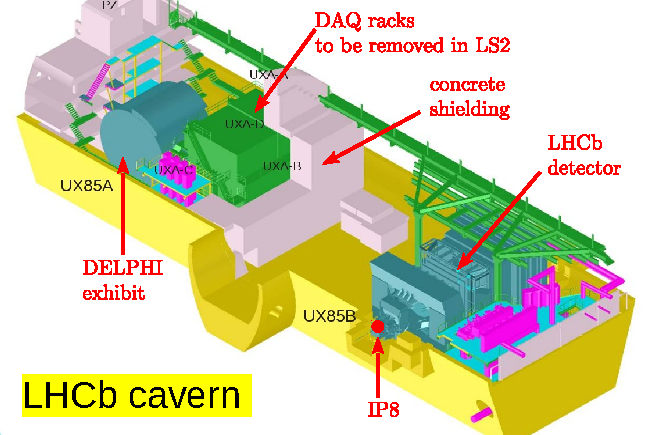
\includegraphics[width=12cm]{figs/INT/lhcb_cavern.pdf}
    \vspace{0.15cm}
\caption{ 
   Schematic plot of LHCb cavern 
}
\end{figure}

\section{Measurement}
\label{sec:Measurement}

%Using two 30 X 30 X 2\cm wrapped plastic scintillators with photomultiplier tube (PMT) attached on iron test stand. 
%Each PMTs receives 1.5 kV high voltage and 350 V bias voltage. 
%Why do we set high voltage to 1.5 kV? Because rate increases with bigger high voltage, but it becomes flat when high voltage larger than 1.5 kV
%The scintillators measure mininum ionizing particles (mip).
%This supports by NIM crate.
%We test this equipments at lab taking cosimc rays
%This is the first time measured hit rate at underground cavern.
%Results from measurments may impact to other LLP experiments.
%When particle goes through scintillators and makes hits on both detectors, we counts number of events. 
%We made 30 mV threshold of signal pick to measure data which has physical meaning. 
%Triggering when signals appear at both detector in 5 ns. 
%Since detector have been placed 100 m below underground, muons from cosmic rays decay are suppressed. 
%We take data during MD and when the beam is online. 
%We switch the detector position several times. Also we take data while detector is rotated. 
%This is the first measurement of hit rate at D3 platform. 
%We use scope to take data, hit rate is not high. 
%We remotely connect to scope and able to manage scope.
%We took data from 4 different places. 
%Back of D3 platform of each corner and central position.
%Front D3 platform at central with parallel to beam line and make 45 degree with a beam line.

\subsection{Test-bench}
We used Herschel detector.
For PMT, model: R1828-01
Because, it has high anode current upper limit, wide range of gain variation, fast time response to fit in 25 ns, large entry window to increase light yield, good single electron separation.
The test-bench includes cosmic stand, scope with extended functions (auto save waveforms, coincidence logic), high voltage power supplies (1.5 kV, bias 350 V), current-voltage meter, laptop to remote connect to scope.

\begin{figure}[h]
\centering
    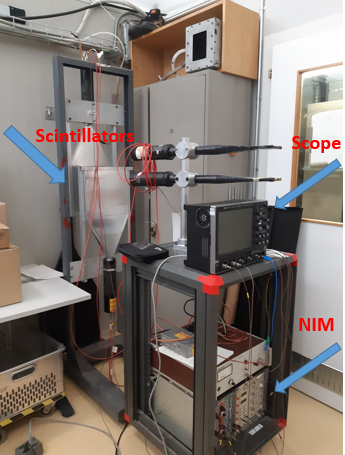
\includegraphics[width=5.5cm]{figs/INT/Tools.png} 
\caption{ 
    Test-bench photo
}
\end{figure}

\subsection{Trigger}
We used simple 2x fold coincidence and a distance between two scintillators 2\cm. 
For this measurment, a discrimination (scope) threshold set as 30 mV.
When first scintillator receive a signal and the other scintillator also receives a signal in 5 ns, scope counts.
The scope automatically saved two waveforms from each scintillator and the number of mininum ionizing particles (mip) counted during the run.

\begin{figure}[h]
\centering
    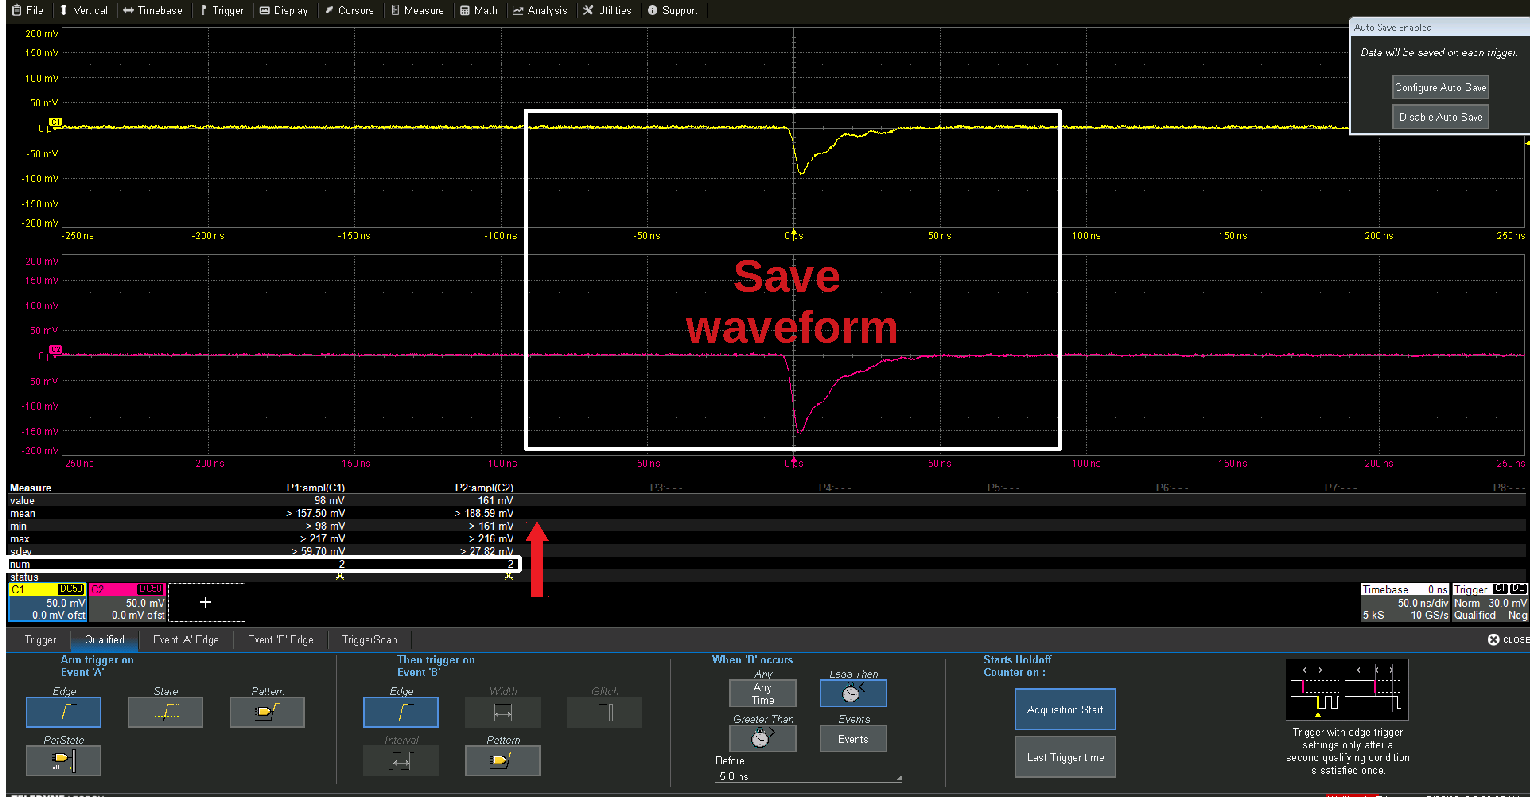
\includegraphics[width=8cm]{figs/INT/waveform.pdf}
\caption{
    Trigger setup using coincidence occurence of two signals in 5~ns. 
}
\end{figure}

\subsection{Detail Configuration}

The background measurement was taken at the LHCb cavern on D3 platform. The equipment had been set at 3 positions between DAQ racks and the concrete shield wall and the position between the \delphi and DAQ racks.
We basically placed the scintillator stand parallel to the beam line but also rotated $45^{\circ}$ and perpendicular to the beam line.
Fig 4. shows positions and configurations of measurement.

\begin{figure}[h]
\centering
    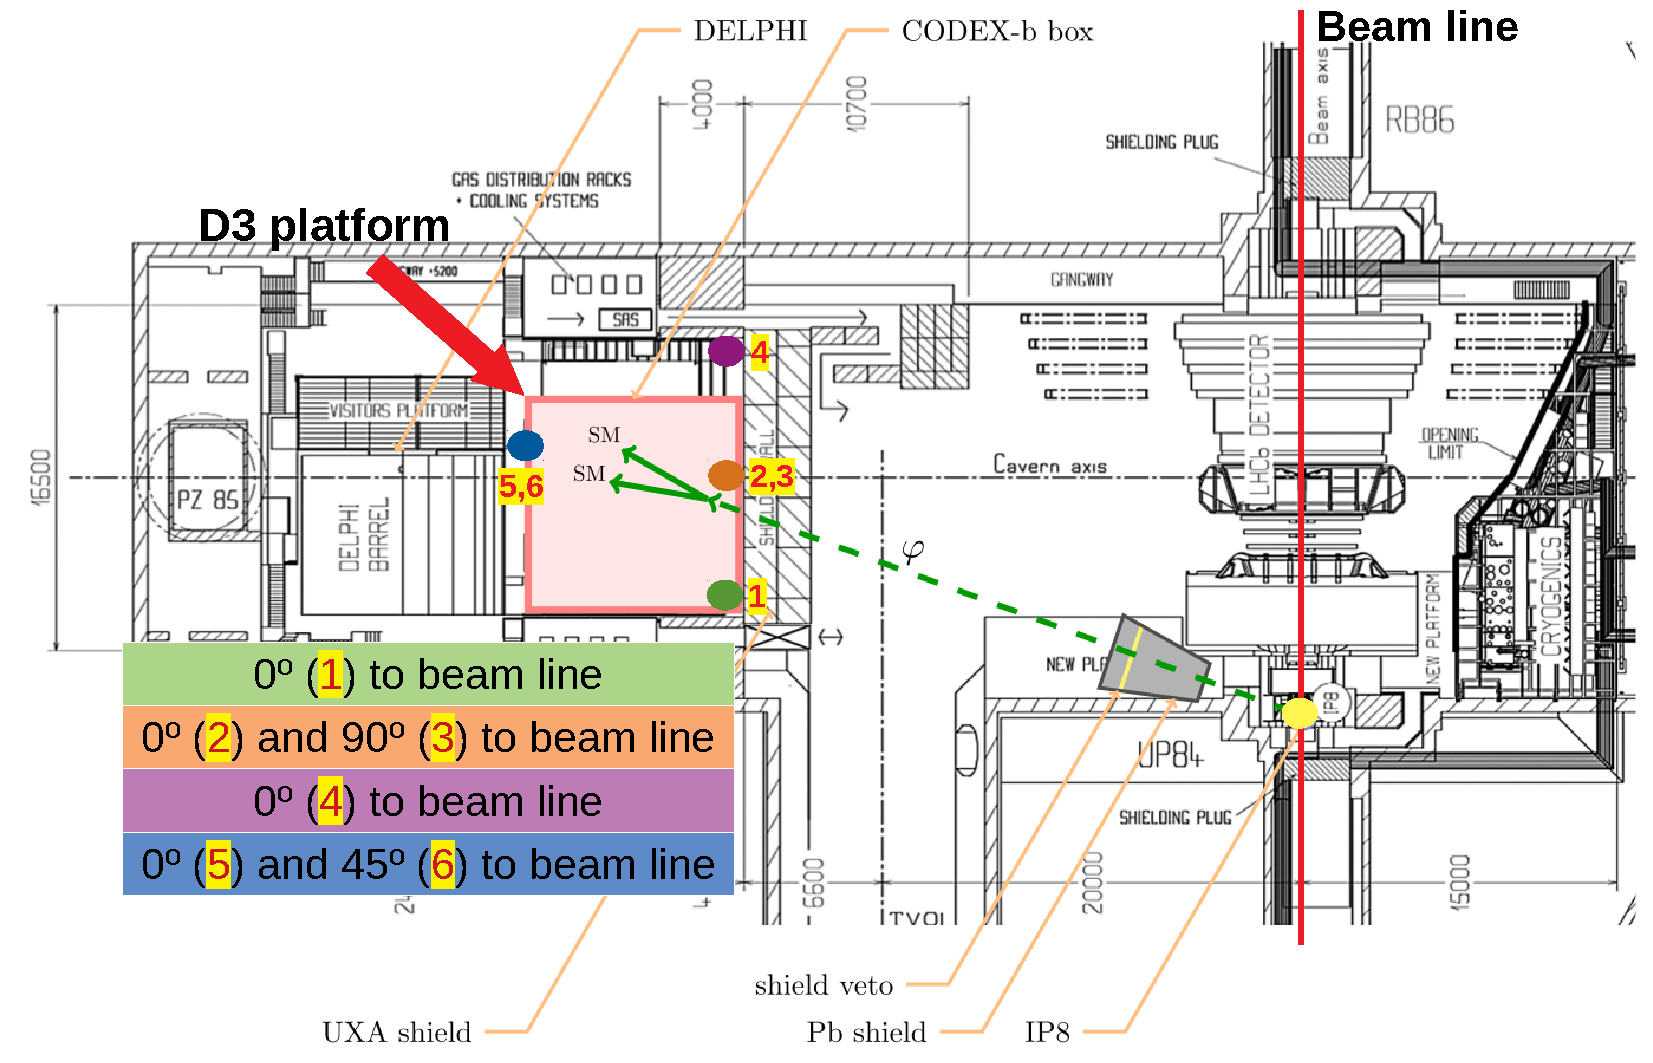
\includegraphics[width=8cm]{figs/INT/configuration.pdf}
\caption{
    Four measurement positions at the LHCb cavern
}
\end{figure}

\subsection{Results}

The measurement campagin spanning 17 days in July-Aug 2018.
The scope performed 52036 triggers during the runi.
The LHCb lumi rate was stable during the measurement.
There was no beam until July 30th because of machine develop and power cut happened during measurement.

\vspace{0.2cm}
\begin{figure}[h]
\centering
    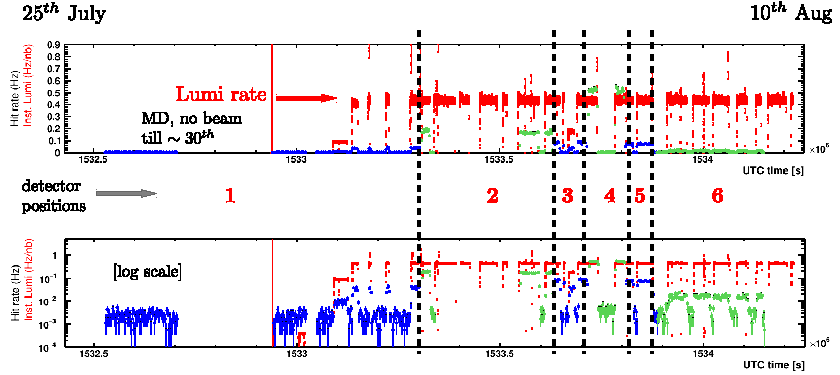
\includegraphics[width=12cm]{figs/INT/codexb_data_global.pdf}
\caption{
    Hit rate plots during the run based on 6 positions/configurations linear and log scale. Red dots mean the lumi rate of \lhcb, blue and green dots mean hit rates.
}
\end{figure}

Below tables are shown hit rate based on measurement position and configuration.
The rate of $pp$ collisions is 25~MHz.
First table is about ambient background hit rate between fills and in MD without beam.

\begin{table}
\begin{center}
\begin{tabular}{c|l|r}
  Position & \hspace{2cm}Description & Hit rate [mHz] \\
  \hline \hline
   P1 & shield, right corner, $\parallel$ to beam& $1.99\pm0.07$ \\ \hline
   P2 & shield, center, $\parallel$ to beam&  $2.76\pm 0.03$ \\ \hline
   P3 & shield, center, $\perp$ to beam& $ 2.26\pm 0.03$ \\ \hline
   P4 & shield, left corner, $\parallel$ to beam& $ 3.11\pm 0.03$ \\ \hline
   P5 & shield + D3 racks, center, $\parallel$ to beam& $ 1.95\pm 0.03$ \\ \hline
   P6 & shield + D3 racks, center, $45^\circ$ to beam& $ 2.22\pm $ 0.02\\ \hline
\end{tabular}
\caption{
    Pure background hit rates based on each configuration
}
\end{center}
\end{table}

The average hit rate of each position and configuration is 2~mHz. 
It is indicated that background can be negligible. 
However, during stable beam, hit rate increases a large.
By moving position from P1 to P2, from P2 to P4, we found that hit rate depends on $\eta$
Also, DAQ racks add some shielding effect based on the hit rates of P5 and P6.

\begin{table}
\begin{center}
\begin{tabular}{c|l|r}
  Position & \hspace{0.9cm}Description & Hit rate [mHz] \\
  \hline \hline
   P1 & shield, right corner, $\parallel$ to beam & $ 38.99 \pm 0.99 $\\ \hline
   P2 & shield, center, $\parallel$ to beam& $ 167.10 \pm 1.43$ \\ \hline
   P3 & shield, center, $\perp$ to beam& $ 82.81 \pm 1.55 $ \\ \hline
   P4 & shield, left corner, $\parallel$ to beam& $ 517.45 \pm 3.52 $ \\ \hline
   P5 & shield + D3 racks, center, $\parallel$ to beam& $ 73.58 \pm 1.18 $ \\ \hline
   P6 & shield + D3 racks, center, $45^\circ$ to beam& $ 15.71 \pm 0.33 $ \\ \hline
\end{tabular}
\caption{
    Average hit rates during the stable beam measured by the Herschel detector
}
\end{center}
\end{table}


\newpage
\begin{figure}[h]
  \begin{center}
    \begin{tabular}[t]{cc}
      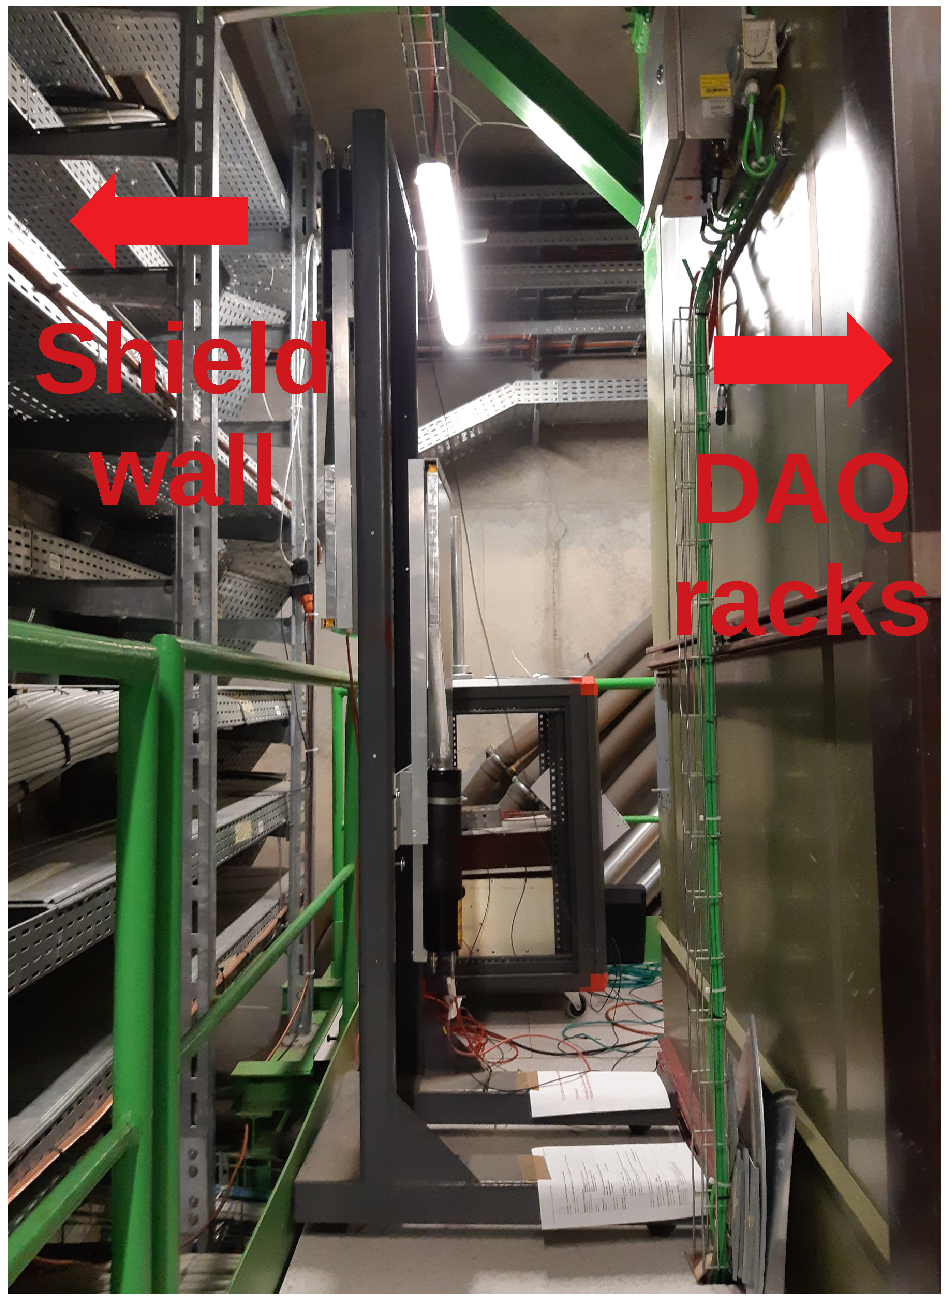
\includegraphics[width=8.5cm]{figs/INT/Initial.pdf} &
      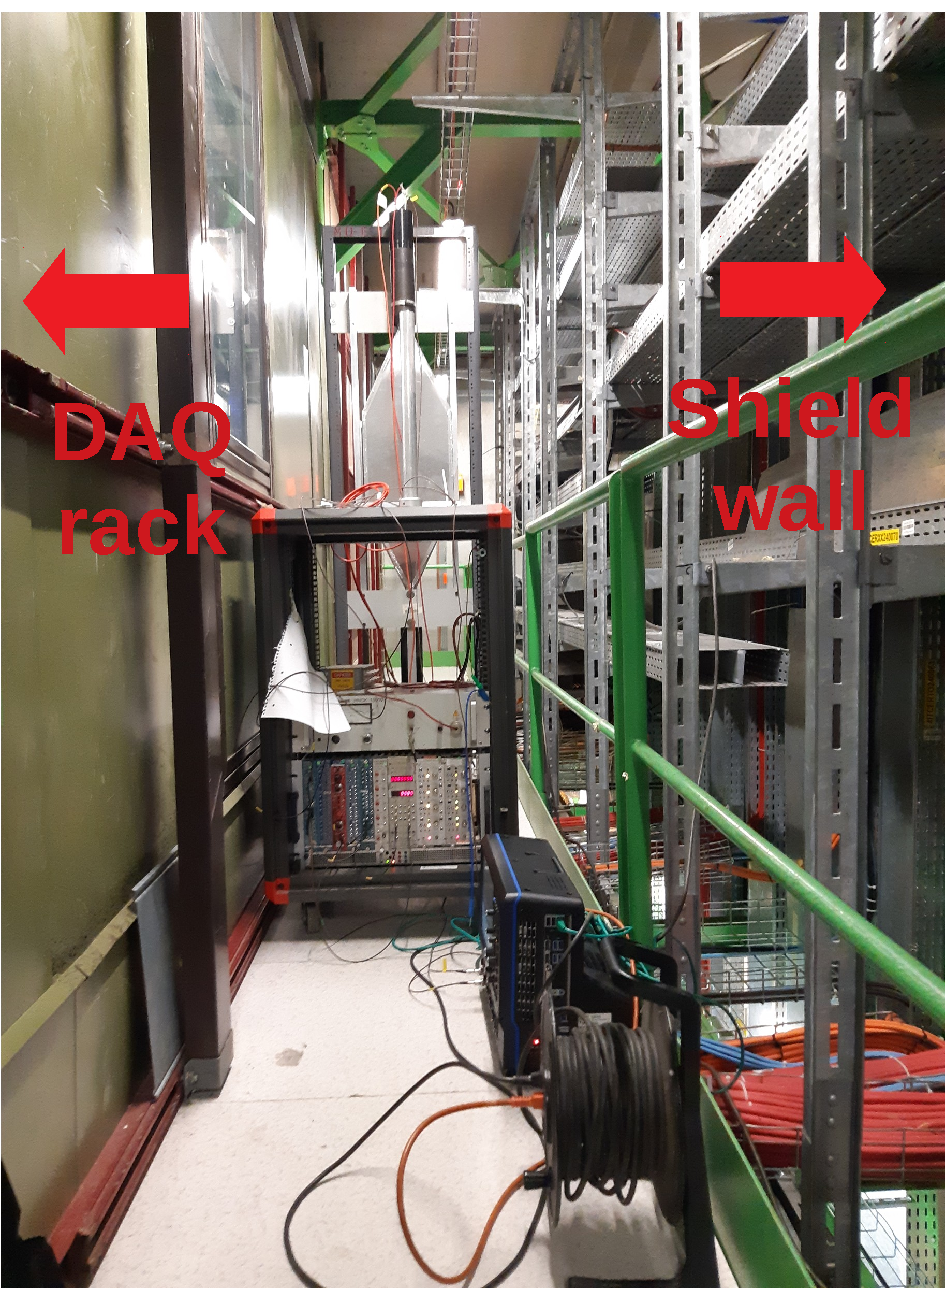
\includegraphics[width=8.5cm]{figs/INT/Back_central.pdf} \\
      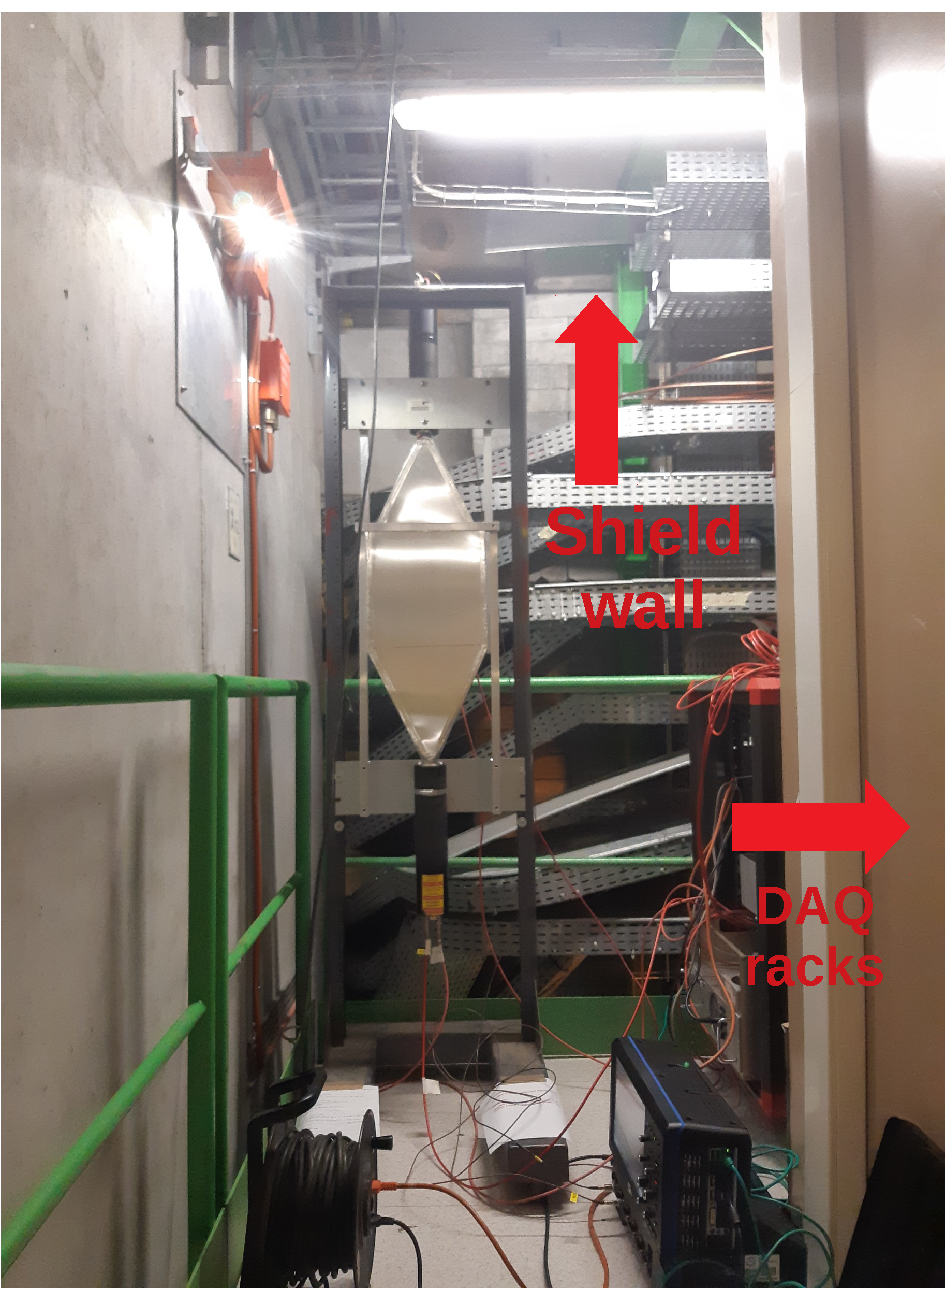
\includegraphics[width=8.5cm]{figs/INT/Othercorner.pdf} &
      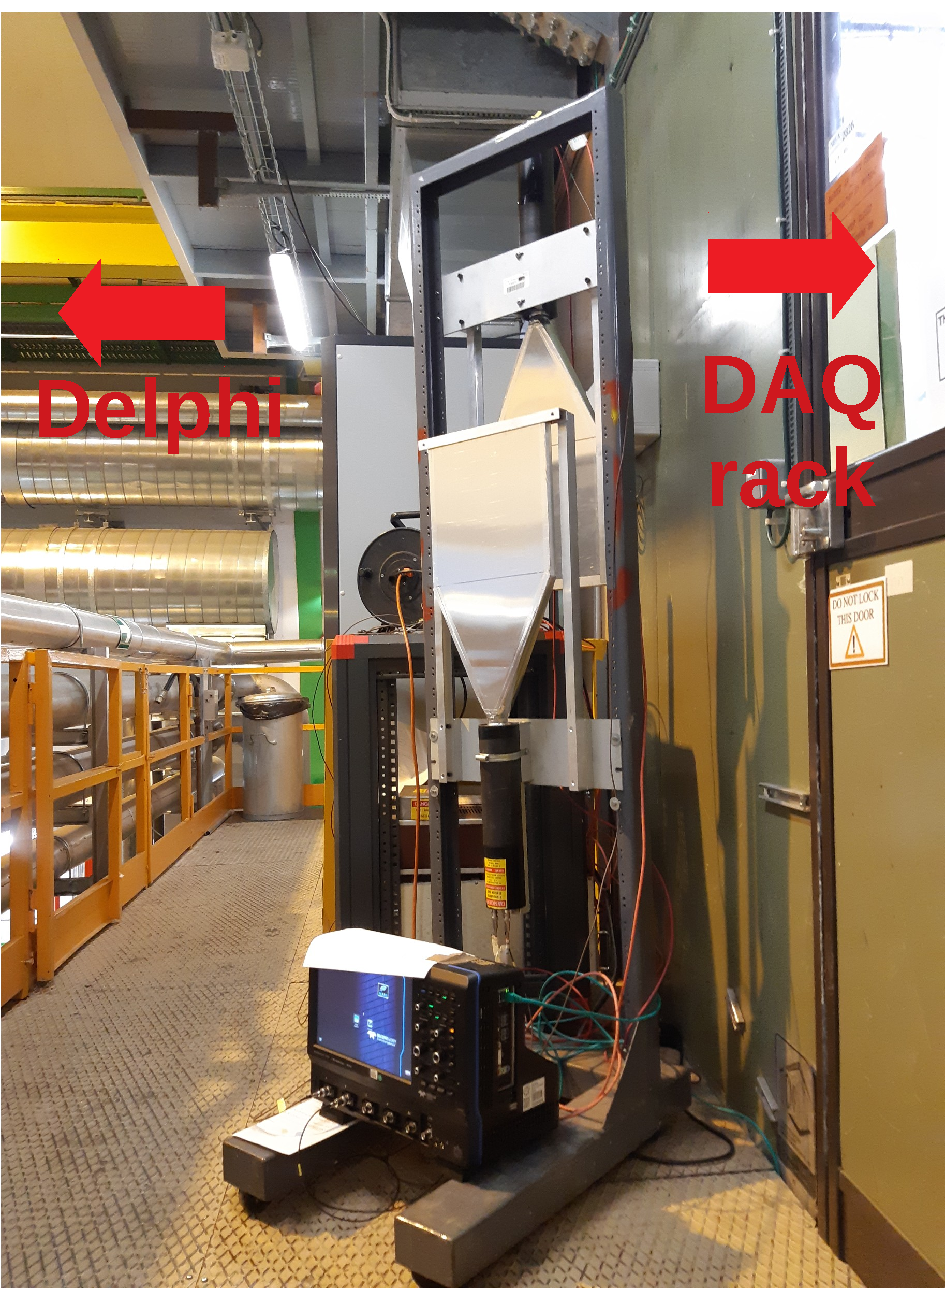
\includegraphics[width=8.5cm]{figs/INT/D3_front.pdf} \\
    \end{tabular}
  \end{center}
\caption{
    Photos from each position at D3 platform
}
\end{figure}

\section{Simulation}
\label{sec:Simulation}

\subsection{Detector Description for High Energy Physics}
We used Detector Description for High Energy Physics (DD4hep) standalone version.
DD4hep is a software framework to provide overall detector description for experiments.
It offers a consistent description through a single source of detector information for simulation, reconstruction, analysis, etc.
Additionally, DD4hep being developed for high luminosity large hadron collider (HL-LHC) detector simulation.
During the internship, we built the geometry of CODEX-b constructing hierachy system.
We designed concrete shield wall to block particles from particle gun or MC and herschel detector since we used as a scintillator for our measurement.
For validation $\mu$ particle gun and minbias event had been used.
We also checked energy deposits and positions of CODEX-b hits. 

%I learn how to make geometry: layer, station, super staion, envelope (hierachy).
%I define materials for our detector and CODEX-b geometry such as concrete, Herschel detector.
%Layer consists of silicon, station consists of aluminum. 
%There is a veto cone with two lead and one silicon. 
%Also just in front of CODEX-b, concrete wall exists to veto muons.
%First of all, using muon particle gun with high energy, test our geometry.
%And then using HepMC to generate pp collisions and do the same process as muon particle gun.
%I made hierachy system to build CODEX-b (envelop, super station, station, layer).
%I could check energy deposits and positions of CODEX-b hits.

\subsection{Simulation geometry}
First geometry is the CODEX-b.
CODEX-b consists of two parts face station and inner station.
Based on the paper, face station has 6 resistive plate chambers (RPCs) layers at 4~cm intervals with 1~cm granularity.
The size of each layer is 10 x 10~$m^{2}$ and the thickness is 2~cm. 
In this simulation we had been implemented layers as a tracker instead of RPCs.
Inner station also has same configuration except number of layers.
It will be equally spaced with triplets along the depth to minimize distance between reconstructed vertex and 1st measurement. 

%To make coincidence setup with test-bench, I made two Herschel plates with the same positions where all equipment have set.
%Two plates with 30 x 30~$cm^{2}$ size, 2~cm thickness.
%There is a concrete wall in front of scintillators.
%3~m thickness to suppress particles from pp collisions.
%Roughly in 1000 events, it has hits on scinitillators 4 - 9 events.
%There is a proposed veto cone. It consists of two lead absorbers and one silicon tracker.
%There is also concrete wall which blocks radiations (or particles) to reach CODEX-b box. 
%It has 3.2~m thickness.

\begin{figure}[h]
\begin{center}
  \begin{tabular}[t]{cc}
    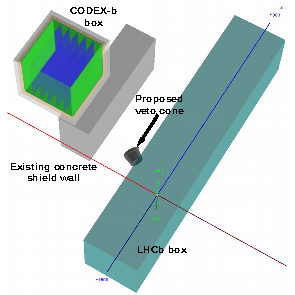
\includegraphics[width=0.5\textwidth]{figs/INT/CODEXbBigGeo.pdf} &
    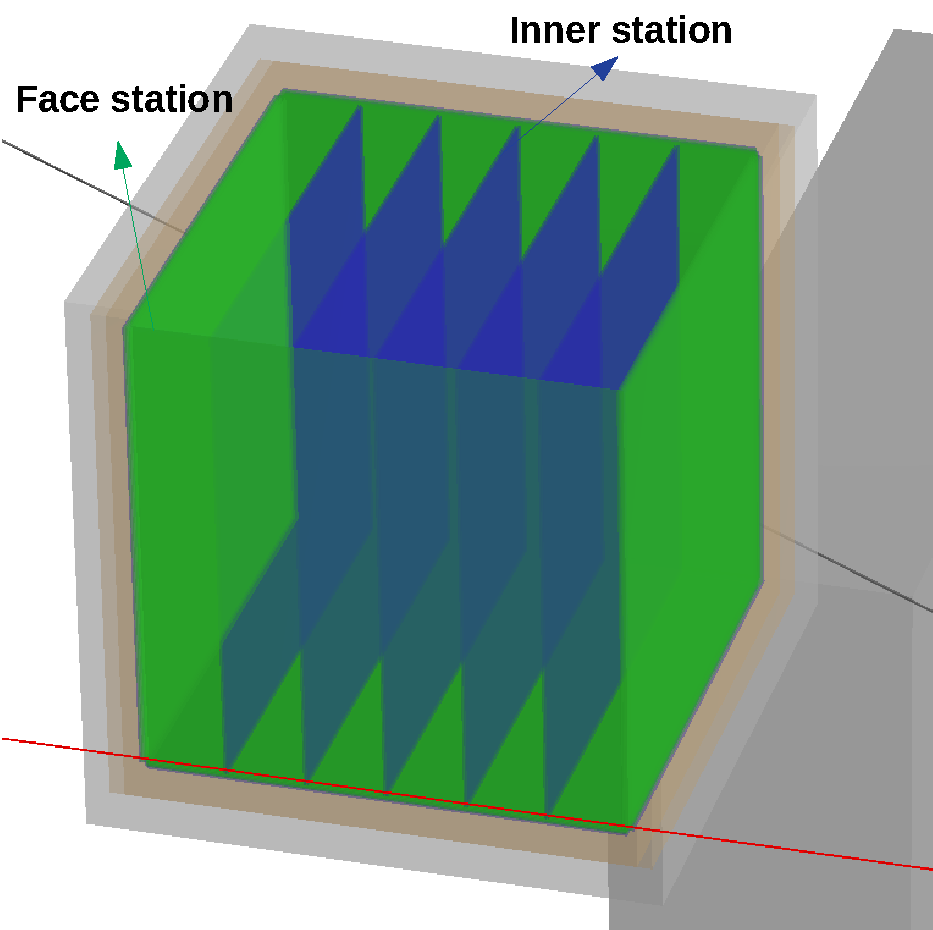
\includegraphics[width=0.5\textwidth]{figs/INT/ZoomVersion.pdf}
  \end{tabular}
\end{center}
\caption{
    Wide view of CODEX-b simulation geometry
}
\end{figure}

We also created a concrete shield wall with 3.2~m thickness.
It was placed just front of CODEX-b box.
Between the LHCb box and the concrete wall, there is a proposed veto cone.
It contains two lead absorber and one active silicon layer.

Second geometry was consists of two scintillator plates which is the same as our measurement configurations.
The material of scintillator was  

\subsection{Simulation status}

We designed two different detectors based on the paper and the measurement, the former is the CODEX-b and the latter is a scintillator.
Both were tested with $\mu$ particle gun with 1\tev and the minimum bias events generated from the standalone Gauss. 

\begin{figure}[h]
\centering
    \begin{tabular}[t]{cc}
    %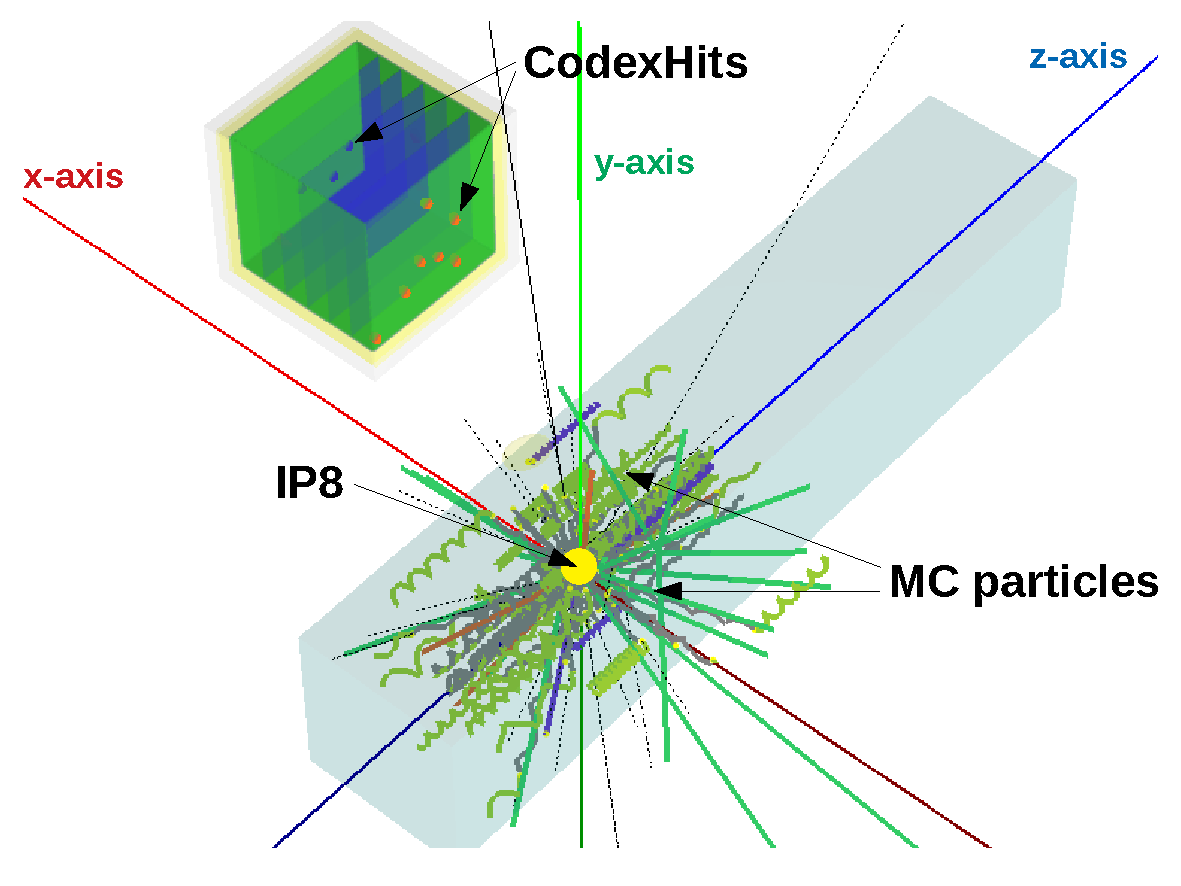
\includegraphics[width=8cm]{figs/INT/Minbias.pdf} \\
    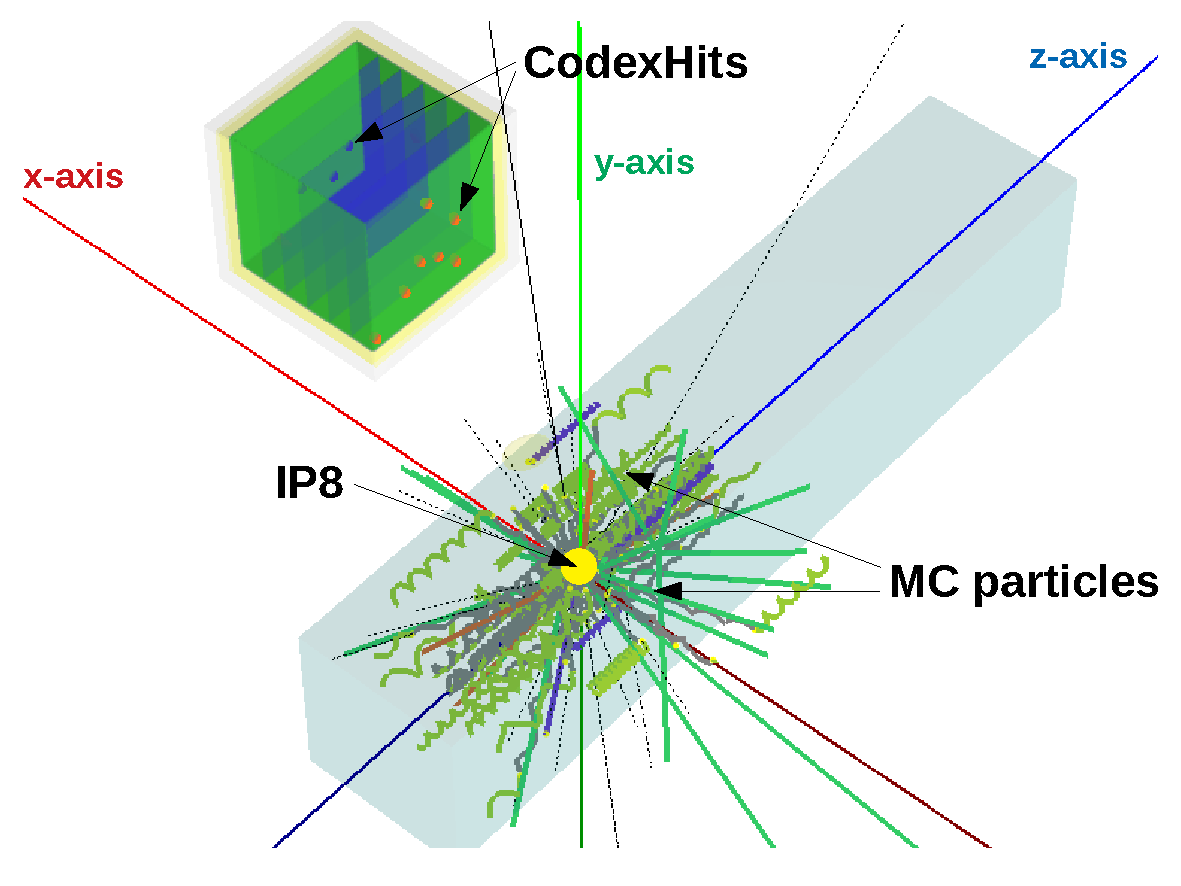
\includegraphics[width=0.65\textwidth]{figs/INT/Minbias.pdf} \\
    \vspace{0.2cm} 
    %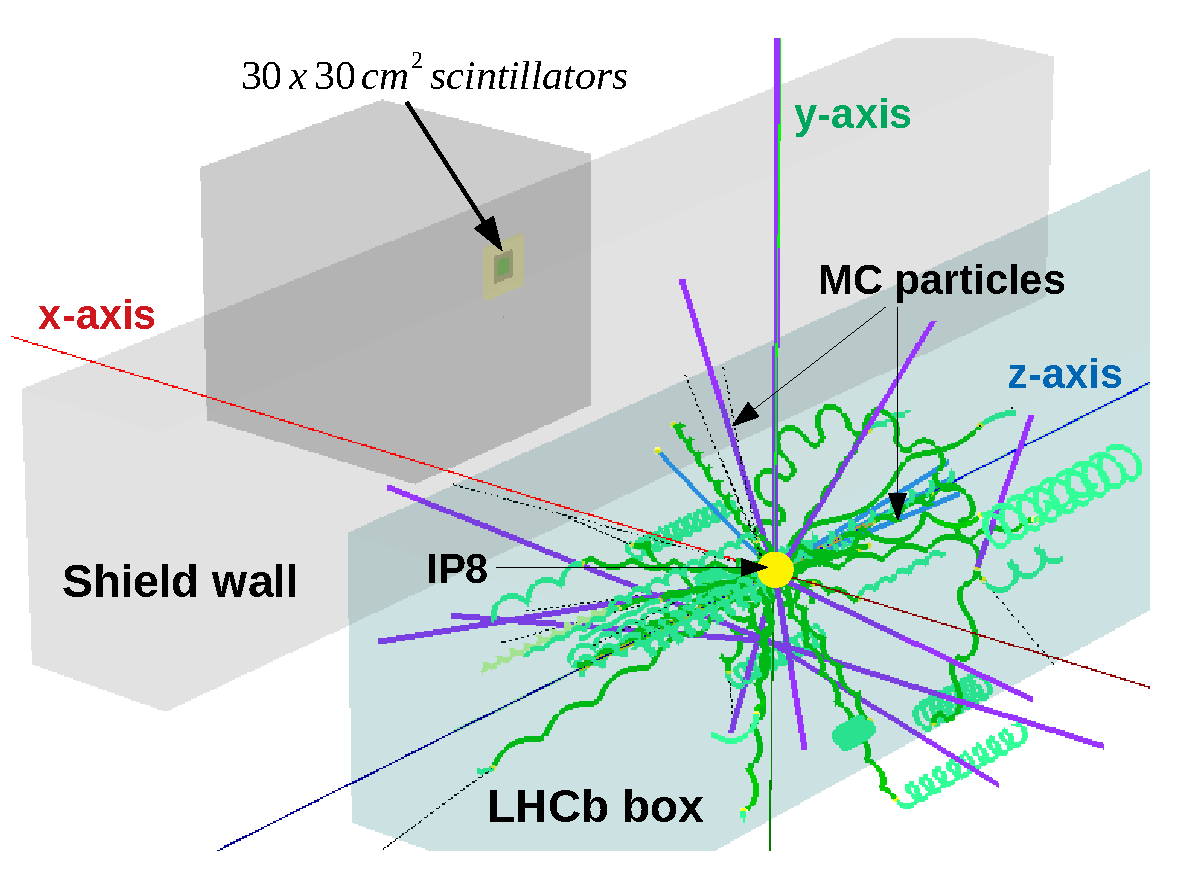
\includegraphics[width=8cm]{figs/INT/Scint.pdf}
    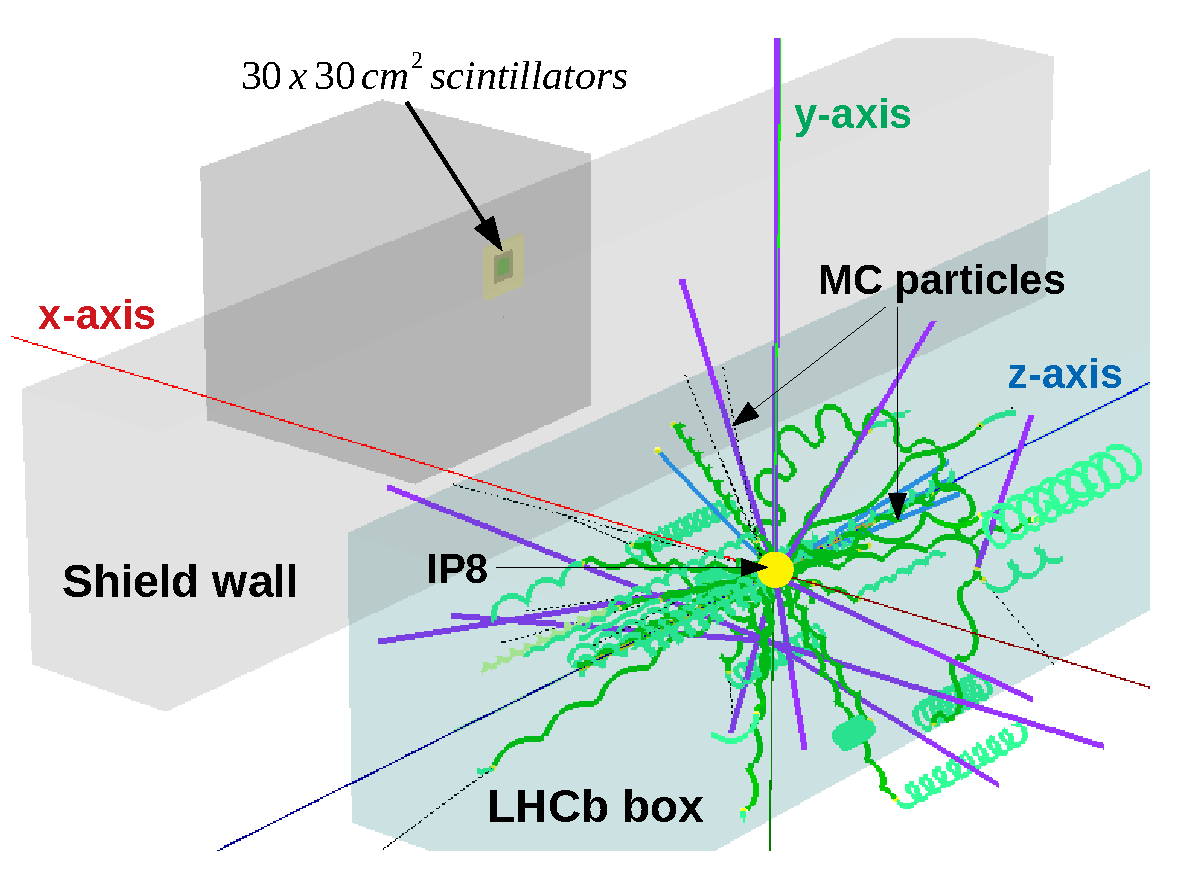
\includegraphics[width=0.65\textwidth]{figs/INT/Scint.pdf}
    \end{tabular}
\caption{
    Validation of the CODEX-b simulation by removing the concrete shield wall with minimum bias events 
}
\end{figure}

%To check hits on the layers of the CODEX-b, we removed the concrete wall. Fig 8 upper plot is shown the results.
There was no hits on the CODEX-b layers when tested minbias events with the concrete wall.
We decided to remove the shield wall to check performance of layers.
The Figure 8 upper plot is shown that hits from minbias events.
Also we recovered the concrete wall and changed CODEX-b geometry to two scintillator plates and tested with minbias events.
Following the lower plot of Fig 8, there is no hit on the scintillators.
Because its size is too small to measure hits and the concrete wall blocks particles from collisions.

%\begin{figure}[h]
%\centering
%\caption{
%    Test of the scintialltor configuration with minimum bias events
%}
%\end{figure}

\section{Summary}

\frame{
    \frametitle{Summary: exotics @ LHCb}
    \vspace{-0.3cm}
    \begin{itemize}
      %\item \textcolor{red}{$X(3872)$}: $J^{PC}=1^{++}$ confirmed, $\Gamma<1.2$~MeV, dominant $P$-wave $[\pi\pi]$ in $X\to \jpsi \pi\pi$, $R_{\psi \gamma}$ rules out pure $D\overline{D}^\ast$.
      %\vspace{0.2cm}
      %\item \textcolor{red}{$Z(4430)^+$}: resonant nature, $J^P =1^+$. $R_{\psi \pi/\psi' \pi}\sim 10$ (\href{https://arxiv.org/abs/1408.6457}{Belle}). Tetraquark candidate (rapidly separating \href{http://arxiv.org/abs/1406.7281}{diquarks}?). 
      %\vspace{0.2cm}
      \item \textcolor{red}{$\Lb\to \jpsi p\Km$}: ``model-independent'' approach confirms $\Lambda^\ast$ reflections can't explain data. Exotics present.
      \vspace{0.5cm}
      \item \textcolor{red}{$\Lb\to \jpsi p\pim$}: $P_c$'s consistent with the $\jpsi p \Km$ mode. $R_{\pi/K}$ consistent with Cabibbo suppression.
      \vspace{0.5cm}
      \item \textcolor{red}{$X\to \jpsi \phi$}: confirms $1^+$ for \textcolor{red}{$X(4140)$} and $X(4274)$. $X(4140)$ width larger than CDF. Two new high-mass $0^+$ resonances. 
      \vspace{0.5cm}
      \item LHCb does {\em not} confirm D0 \textcolor{red}{$X(5568)$}. Inputs from ATLAS/CMS?
    \end{itemize}
    \centering

}

\frame{
    \frametitle{Summary: $B_c^+$ physics @ LHCb}
    \vspace{-0.3cm}
    \begin{itemize}
       \item LHCb has performed many measurements in $B_c^+$ physics in Run~I
       \vspace{0.3cm}
       \item Most precise \textcolor{red}{mass} and \textcolor{red}{lifetime} measurements.
       \vspace{0.3cm}
       \item Many \textcolor{red}{decay modes} observed: $\jpsi 3\pi$, $\jpsi\Km$, $\psi(2s)\pi$, $\jpsi D_s^{(*)+}$, $\jpsi 2K\pi$, $\jpsi 3\pi 2\pi$, $\B_s\pi$, ...
       \vspace{0.3cm}
        \item New modes being investigated, especially charmless weak \textcolor{red}{annihilation} types.
        \vspace{0.3cm}
        \item Searches for \textcolor{red}{excited $B_c$} states ongoing as well.
    \end{itemize}
    \pause
    \centering
\begin{tcolorbox}[width=4.5in,height=0.36in,colback=white,colframe=red]
	\textcolor{red}{$\times 5$} statistics after Run~II (end-2018). Much more data coming!.
\end{tcolorbox}
}


\section*{Acknowledgements}
%
% These Acknowledgements valid from 6-July-2018
%
\noindent We express our gratitude to our colleagues in the CERN
accelerator departments for the excellent performance of the LHC. We
thank the technical and administrative staff at the LHCb
institutes.
We acknowledge support from CERN and from the national agencies:
CAPES, CNPq, FAPERJ and FINEP (Brazil); 
MOST and NSFC (China); 
CNRS/IN2P3 (France); 
BMBF, DFG and MPG (Germany); 
INFN (Italy); 
NWO (Netherlands); 
MNiSW and NCN (Poland); 
MEN/IFA (Romania); 
MinES and FASO (Russia); 
MinECo (Spain); 
SNSF and SER (Switzerland); 
NASU (Ukraine); 
STFC (United Kingdom); 
NSF (USA).
We acknowledge the computing resources that are provided by CERN, IN2P3
(France), KIT and DESY (Germany), INFN (Italy), SURF (Netherlands),
PIC (Spain), GridPP (United Kingdom), RRCKI and Yandex
LLC (Russia), CSCS (Switzerland), IFIN-HH (Romania), CBPF (Brazil),
PL-GRID (Poland) and OSC (USA).
We are indebted to the communities behind the multiple open-source
software packages on which we depend.
Individual groups or members have received support from
AvH Foundation (Germany);
EPLANET, Marie Sk\l{}odowska-Curie Actions and ERC (European Union);
ANR, Labex P2IO and OCEVU, and R\'{e}gion Auvergne-Rh\^{o}ne-Alpes (France);
Key Research Program of Frontier Sciences of CAS, CAS PIFI, and the Thousand Talents Program (China);
RFBR, RSF and Yandex LLC (Russia);
GVA, XuntaGal and GENCAT (Spain);
the Royal Society
and the Leverhulme Trust (United Kingdom);
Laboratory Directed Research and Development program of LANL (USA).



% Do not include this in any draft (just for information in the template)
%\section{Acknowledgements paragraph}

Include the following text in the Acknowledgements section in all paper
drafts. It is not needed for analysis notes or conference reports.

The text below are the acknowledgements as approved by the collaboration
board. Extending the acknowledgements to include individuals from outside the
collaboration who have contributed to the analysis should be approved by the
EB. The extra acknowledgements are normally placed before the standard 
acknowledgements, unless it matches better with the text of the standard 
acknowledgements to put them elsewhere. They should be included in the draft 
for the first circulation. Except in exceptional circumstances, to be approved by the
EB chair, authors of the paper should not be named in extended acknowledgements.

%\vspace{1cm}

\section*{Acknowledgements}
%
% These Acknowledgements valid from 6-July-2018
%
\noindent We express our gratitude to our colleagues in the CERN
accelerator departments for the excellent performance of the LHC. We
thank the technical and administrative staff at the LHCb
institutes.
We acknowledge support from CERN and from the national agencies:
CAPES, CNPq, FAPERJ and FINEP (Brazil); 
MOST and NSFC (China); 
CNRS/IN2P3 (France); 
BMBF, DFG and MPG (Germany); 
INFN (Italy); 
NWO (Netherlands); 
MNiSW and NCN (Poland); 
MEN/IFA (Romania); 
MinES and FASO (Russia); 
MinECo (Spain); 
SNSF and SER (Switzerland); 
NASU (Ukraine); 
STFC (United Kingdom); 
NSF (USA).
We acknowledge the computing resources that are provided by CERN, IN2P3
(France), KIT and DESY (Germany), INFN (Italy), SURF (Netherlands),
PIC (Spain), GridPP (United Kingdom), RRCKI and Yandex
LLC (Russia), CSCS (Switzerland), IFIN-HH (Romania), CBPF (Brazil),
PL-GRID (Poland) and OSC (USA).
We are indebted to the communities behind the multiple open-source
software packages on which we depend.
Individual groups or members have received support from
AvH Foundation (Germany);
EPLANET, Marie Sk\l{}odowska-Curie Actions and ERC (European Union);
ANR, Labex P2IO and OCEVU, and R\'{e}gion Auvergne-Rh\^{o}ne-Alpes (France);
Key Research Program of Frontier Sciences of CAS, CAS PIFI, and the Thousand Talents Program (China);
RFBR, RSF and Yandex LLC (Russia);
GVA, XuntaGal and GENCAT (Spain);
the Royal Society
and the Leverhulme Trust (United Kingdom);
Laboratory Directed Research and Development program of LANL (USA).



% Comment this in for paper darfts; do not include this in analysis note and conference reports
%\section*{Acknowledgements}
%
% These Acknowledgements valid from 6-July-2018
%
\noindent We express our gratitude to our colleagues in the CERN
accelerator departments for the excellent performance of the LHC. We
thank the technical and administrative staff at the LHCb
institutes.
We acknowledge support from CERN and from the national agencies:
CAPES, CNPq, FAPERJ and FINEP (Brazil); 
MOST and NSFC (China); 
CNRS/IN2P3 (France); 
BMBF, DFG and MPG (Germany); 
INFN (Italy); 
NWO (Netherlands); 
MNiSW and NCN (Poland); 
MEN/IFA (Romania); 
MinES and FASO (Russia); 
MinECo (Spain); 
SNSF and SER (Switzerland); 
NASU (Ukraine); 
STFC (United Kingdom); 
NSF (USA).
We acknowledge the computing resources that are provided by CERN, IN2P3
(France), KIT and DESY (Germany), INFN (Italy), SURF (Netherlands),
PIC (Spain), GridPP (United Kingdom), RRCKI and Yandex
LLC (Russia), CSCS (Switzerland), IFIN-HH (Romania), CBPF (Brazil),
PL-GRID (Poland) and OSC (USA).
We are indebted to the communities behind the multiple open-source
software packages on which we depend.
Individual groups or members have received support from
AvH Foundation (Germany);
EPLANET, Marie Sk\l{}odowska-Curie Actions and ERC (European Union);
ANR, Labex P2IO and OCEVU, and R\'{e}gion Auvergne-Rh\^{o}ne-Alpes (France);
Key Research Program of Frontier Sciences of CAS, CAS PIFI, and the Thousand Talents Program (China);
RFBR, RSF and Yandex LLC (Russia);
GVA, XuntaGal and GENCAT (Spain);
the Royal Society
and the Leverhulme Trust (United Kingdom);
Laboratory Directed Research and Development program of LANL (USA).


%% $Id: appendix.tex 121372 2018-06-20 13:32:23Z pkoppenb $
% ===============================================================================
% Purpose: appendix to the standard template: standard symbol alises from Ulrik
% Author: Tomasz Skwarnicki
% Created on: 2009-09-24
% ===============================================================================

%{\noindent\normalfont\bfseries\Large Appendices}
\section*{Appendices}

\appendix

\section{Standard References}
\label{sec:StandardReferences}
Below is a list of common references, as
well as a list of all \lhcb publications. 
As they are already in prepared bib files, they can be used as simply as
\texttt{\textbackslash cite\{Alves:2008zz\}} to get the \lhcb detector paper. 
The references are defined in the files \texttt{main.bib},  \texttt{LHCb-PAPER.bib},
\texttt{LHCb-CONF.bib}, \texttt{LHCb-DP.bib} \texttt{LHCb-TDR.bib} files, with obvious contents.
Each of these have their \texttt{LHCb-ZZZ-20XX-0YY} number as their cite code.
If you believe there is a problem with the formatting or
content of one of the entries, then get in contact with the Editorial
Board rather than just editing it in your local file,
since you are likely to need the latest version just before submiting the article.

\begin{center}
  \begin{longtable}{llc}
\caption{\small Standard references.}\label{tab:Refs}
\endfirsthead
\multicolumn{3}{c}{ -- continued from previous page.}
\endhead
\endfoot
\endlastfoot
\hline
Description & \texttt{cite} code & Reference \\
\hline
\lhcb detector & \texttt{Alves:2008zz} & \cite{Alves:2008zz} \\
%% Trigger & \texttt{LHCb-DP-2012-004} & \cite{LHCb-DP-2012-004} \\
%% RICH & \texttt{LHCb-DP-2012-003} & \cite{LHCb-DP-2012-003} \\
%% PID performance & \texttt{LHCb-PROC-2011-008} & \cite{LHCb-PROC-2011-008} \\
\lhcb simulation & \texttt{LHCb-PROC-2011-006} & \cite{LHCb-PROC-2011-006} \\
PDG 2018 & \texttt{PDG2018} & \cite{PDG2018} \\
PDG 2016 & \texttt{PDG2016} & \cite{PDG2016} \\
PDG 2014 & \texttt{PDG2014} & \cite{PDG2014} \\
HFLAV 2016 & \texttt{HFLAV16} & \cite{HFLAV16} \\
HFAG (pre-2016)  & \texttt{Amhis:2014hma} & \cite{Amhis:2014hma} \\
\pythia & \texttt{Sjostrand:2006za, *Sjostrand:2007gs} & \cite{Sjostrand:2006za, *Sjostrand:2007gs} \\
\lhcb \pythia tuning & \texttt{LHCb-PROC-2010-056} & \cite{LHCb-PROC-2010-056} \\
\geant & \texttt{Allison:2006ve, *Agostinelli:2002hh} & \cite{Allison:2006ve, *Agostinelli:2002hh} \\
\evtgen & \texttt{Lange:2001uf}  & \cite{Lange:2001uf} \\
\photos & \texttt{Golonka:2005pn}  & \cite{Golonka:2005pn} \\
\dirac & \texttt{Tsaregorodtsev:2010zz, *BelleDIRACAmazon} & \cite{Tsaregorodtsev:2010zz, *BelleDIRAC}  \\
Crystal Ball function\footnote{A valid alternative for most papers where the normalisation is not critical is to use the expression``Gaussian function with a low-mass power-law tail'' or ``Gaussian function with power-law tails''. In that case, no citation is needed} & \texttt{Skwarnicki:1986xj} & \cite{Skwarnicki:1986xj} \\
Hypatia & \texttt{Santos:2013gra} & \cite{Santos:2013gra}\\
Wilks' theorem & \texttt{Wilks:1938dza} & \cite{Wilks:1938dza}\\
Blatt--Weisskopf barrier & \texttt{Blatt:1952ije} & \cite{Blatt:1952ije} \\
BDT & \texttt{Breiman} & \cite{Breiman} \\
BDT training & \texttt{AdaBoost} & \cite{AdaBoost} \\
TMVA\footnote{Do not cite this instead of the actual reference for the MVA being used.}  & \texttt{Hocker:2007ht,*TMVA4} & \cite{Hocker:2007ht,*TMVA4} \\
HLT2 topo & \texttt{BBDT} & \cite{BBDT} \\
PIDCalib (for Run~1) & \texttt{LHCb-PUB-2016-021} & \cite{LHCb-PUB-2016-021} \\
DecayTreeFitter & \texttt{Hulsbergen:2005pu} & \cite{Hulsbergen:2005pu} \\
\sPlot & \texttt{Pivk:2004ty} & \cite{Pivk:2004ty} \\
Punzi's optimization & \texttt{Punzi:2003bu} & \cite{Punzi:2003bu} \\
$f_s/f_d$ & \texttt{fsfd} & \cite{fsfd} \\
LHC beam energy uncertainty  & \texttt{PhysRevAccelBeams.20.081003} & \cite{PhysRevAccelBeams.20.081003}\\
CL$_s$ method & \texttt{CLs} & \cite{CLs} \\
CKMfitter group & \texttt{CKMfitter2005} & \cite{CKMfitter2005} \\
CKMfitter group & \texttt{CKMfitter2015} & \cite{CKMfitter2015} \\
UTfit (Standard Model/CKM) & \texttt{UTfit-UT} & \cite{UTfit-UT} \\
UTfit (New Physics) & \texttt{UTfit-NP} & \cite{UTfit-NP} \\
Scikit & \texttt{Scikit} & \cite{Scikit} \\
RooUnfold & \texttt{Adye:2011gm} & \cite{Adye:2011gm} \\
EW Baryogenesis \& \CP &  \texttt{Huet:1994jb} & \cite{Huet:1994jb} \\
Baryon asymmetry \& SM \CP &  \texttt{Gavela:1994dt} & \cite{Gavela:1994dt} \\
Baryon asymmetry \& SM \CP &  \texttt{Gavela:1993ts} & \cite{Gavela:1993ts} \\
\texttt{hep-ml} & \texttt{Rogozhnikov:2016bdp} & \cite{Rogozhnikov:2016bdp} \\
Bootstrapping & \texttt{efron:1979} & \cite{efron:1979} \\
\hline
\end{longtable}
%  \end{tabular}
\end{center}

\begin{center}
\begin{longtable}{ll}
\caption{\small LHCb detector performance papers.}\label{tab:LHCb-DPs}
\endfirsthead
\multicolumn{2}{c}{ -- continued from previous page.}
\endhead
\endfoot
\endlastfoot
\hline
    \hline
    \texttt{LHCb-DP} number & Title \\
    \hline
    \texttt{LHCb-DP-2018-002}~\cite{LHCb-DP-2018-002} &
    {\small VeLo material map using SMOG}\\
    \texttt{LHCb-DP-2018-001}~\cite{LHCb-DP-2018-001} &
    {\small PIDCalib for Run 2} (use Ref.~\cite{LHCb-PUB-2016-021} for Run~1) \\
    \texttt{LHCb-DP-2017-001}~\cite{LHCb-DP-2017-001}&
    {\small Performance of the Outer Tracker - Run 2}\\
    \texttt{LHCb-DP-2016-003}~\cite{LHCb-DP-2016-003} &
    {\small HeRSCheL} \\
    \texttt{LHCb-PROC-2015-018}~\cite{LHCb-PROC-2015-018} &
    {\small Topological trigger reoptimization - Run 2} \\
    \texttt{LHCb-PROC-2015-011}~\cite{LHCb-PROC-2015-011} &
    {\small Turbo and real-time alignment - Run 2} \\
    \texttt{LHCb-DP-2016-001}~\cite{LHCb-DP-2016-001} &
    {\small TESLA project - Run 2} \\
    \texttt{LHCb-DP-2014-002}~\cite{LHCb-DP-2014-002} &
    {\small LHCb detector performance} \\
    \texttt{LHCb-DP-2014-001}~\cite{LHCb-DP-2014-001} &
    {\small Performance of the LHCb Vertex Locator} \\
    \texttt{LHCb-DP-2013-004}~\cite{LHCb-DP-2013-004} &
    {\small Performance of the LHCb calorimeters} \\
    \texttt{LHCb-DP-2013-003}~\cite{LHCb-DP-2013-003} &
    {\small Performance of the LHCb Outer Tracker} \\
    \texttt{LHCb-DP-2013-002}~\cite{LHCb-DP-2013-002} &
    {\small Measurement of the track reconstruction efficiency at LHCb} \\
    \texttt{LHCb-DP-2013-001}~\cite{LHCb-DP-2013-001} &
    {\small Performance of the muon identification at LHCb} \\
    \texttt{LHCb-DP-2012-005}~\cite{LHCb-DP-2012-005} &
    {\small Radiation damage in the LHCb Vertex Locator} \\
    \texttt{LHCb-DP-2012-004}~\cite{LHCb-DP-2012-004} &
    {\small The \lhcb trigger and its performance in 2011} \\
    \texttt{LHCb-DP-2012-003}~\cite{LHCb-DP-2012-003} &
    {\small Performance of the \lhcb RICH detector at the LHC} \\
    \texttt{LHCb-DP-2012-002}~\cite{LHCb-DP-2012-002} &
    {\small Performance of the LHCb muon system} \\
    \texttt{LHCb-DP-2012-001}~\cite{LHCb-DP-2012-001} &
    {\small Radiation hardness of the LHCb Outer Tracker} \\
    \texttt{LHCb-DP-2011-002}~\cite{LHCb-DP-2011-002} &
    {\small Simulation of machine induced background ...} \\
    \texttt{LHCb-DP-2011-001}~\cite{LHCb-DP-2011-001} &
    {\small Performance of the LHCb muon system with cosmic rays} \\
    \texttt{LHCb-DP-2010-001}~\cite{LHCb-DP-2010-001} &
    {\small First spatial alignment of the LHCb VELO ...} \\
    \hline
  \end{longtable}
\end{center}

\begin{center}
\begin{longtable}{ll}
\caption{\small LHCb TDRs.}\label{tab:LHCb-TDRs}
\endfirsthead
\multicolumn{2}{c}{ -- continued from previous page.}
\endhead
\endfoot
\endlastfoot
    \hline
    \texttt{LHCb-TDR} number & Title \\
    \hline
    \texttt{LHCb-PII-Physics}~\cite{LHCb-PII-Physics} &
    {\small  Phase-II upgrade physics case} \\
    \texttt{LHCb-PII-EoI}~\cite{LHCb-PII-EoI} &
    {\small Expression of interest for Phase-II upgrade} \\
    \texttt{LHCb-TDR-016}~\cite{LHCb-TDR-016} &
    {\small Trigger and online upgrade} \\
    \texttt{LHCb-TDR-015}~\cite{LHCb-TDR-015} &
    {\small Tracker upgrade} \\
    \texttt{LHCb-TDR-014}~\cite{LHCb-TDR-014} &
    {\small PID upgrade} \\
    \texttt{LHCb-TDR-013}~\cite{LHCb-TDR-013} &
    {\small VELO upgrade} \\
    \texttt{LHCb-TDR-012}~\cite{LHCb-TDR-012} &
    {\small Framework TDR for the upgrade} \\
    \texttt{LHCb-TDR-011}~\cite{LHCb-TDR-011} &
    {\small Computing} \\
    \texttt{LHCb-TDR-010}~\cite{LHCb-TDR-010} &
    {\small Trigger} \\
    \texttt{LHCb-TDR-009}~\cite{LHCb-TDR-009} &
    {\small Reoptimized detector} \\
    \texttt{LHCb-TDR-008}~\cite{LHCb-TDR-008} &
    {\small Inner Tracker} \\
    \texttt{LHCb-TDR-007}~\cite{LHCb-TDR-007} &
    {\small Online, DAQ, ECS} \\
    \texttt{LHCb-TDR-006}~\cite{LHCb-TDR-006} &
    {\small Outer Tracker} \\
    \texttt{LHCb-TDR-005}~\cite{LHCb-TDR-005} &
    {\small VELO} \\
    \texttt{LHCb-TDR-004}~\cite{LHCb-TDR-004} &
    {\small Muon system} \\
    \texttt{LHCb-TDR-003}~\cite{LHCb-TDR-003} &
    {\small RICH} \\
    \texttt{LHCb-TDR-002}~\cite{LHCb-TDR-002} &
    {\small Calorimeters} \\
    \texttt{LHCb-TDR-001}~\cite{LHCb-TDR-001} &
    {\small Magnet} \\
    \hline
  \end{longtable}
\end{center}

\begin{center}
%  \begin{tabular}{l|l}
\begin{longtable}{ll}
\caption{\small
  LHCb-PAPERs (which have their identifier as their cite code).  
  Note that LHCb-PAPER-2011-039 does not exist.
}
\label{tab:LHCb-PAPERs}
\endfirsthead
\multicolumn{2}{c}{ -- continued from previous page.}
\endhead
\endfoot
\endlastfoot
\texttt{LHCb-PAPER-2018-038}~\cite{LHCb-PAPER-2018-038}  &
\texttt{LHCb-PAPER-2018-037}~\cite{LHCb-PAPER-2018-037} \\
\texttt{LHCb-PAPER-2018-036}~\cite{LHCb-PAPER-2018-036}  &
\texttt{LHCb-PAPER-2018-035}~\cite{LHCb-PAPER-2018-035} \\
\texttt{LHCb-PAPER-2018-034}~\cite{LHCb-PAPER-2018-034}  &
\texttt{LHCb-PAPER-2018-033}~\cite{LHCb-PAPER-2018-033} \\
\texttt{LHCb-PAPER-2018-032}~\cite{LHCb-PAPER-2018-032}  &
\texttt{LHCb-PAPER-2018-031}~\cite{LHCb-PAPER-2018-031} \\
\texttt{LHCb-PAPER-2018-030}~\cite{LHCb-PAPER-2018-030}  &
\texttt{LHCb-PAPER-2018-029}~\cite{LHCb-PAPER-2018-029} \\
\texttt{LHCb-PAPER-2018-028}~\cite{LHCb-PAPER-2018-028}  &
\texttt{LHCb-PAPER-2018-027}~\cite{LHCb-PAPER-2018-027} \\
\texttt{LHCb-PAPER-2018-026}~\cite{LHCb-PAPER-2018-026}  &
\texttt{LHCb-PAPER-2018-025}~\cite{LHCb-PAPER-2018-025} \\
\texttt{LHCb-PAPER-2018-024}~\cite{LHCb-PAPER-2018-024}  &
\texttt{LHCb-PAPER-2018-023}~\cite{LHCb-PAPER-2018-023} \\
\texttt{LHCb-PAPER-2018-022}~\cite{LHCb-PAPER-2018-022}  &
\texttt{LHCb-PAPER-2018-021}~\cite{LHCb-PAPER-2018-021} \\
\texttt{LHCb-PAPER-2018-020}~\cite{LHCb-PAPER-2018-020}  &
\texttt{LHCb-PAPER-2018-019}~\cite{LHCb-PAPER-2018-019} \\
\texttt{LHCb-PAPER-2018-018}~\cite{LHCb-PAPER-2018-018}  &
\texttt{LHCb-PAPER-2018-017}~\cite{LHCb-PAPER-2018-017} \\
\texttt{LHCb-PAPER-2018-016}~\cite{LHCb-PAPER-2018-016}  &
\texttt{LHCb-PAPER-2018-015}~\cite{LHCb-PAPER-2018-015} \\
\texttt{LHCb-PAPER-2018-014}~\cite{LHCb-PAPER-2018-014}  &
\texttt{LHCb-PAPER-2018-013}~\cite{LHCb-PAPER-2018-013} \\
\texttt{LHCb-PAPER-2018-012}~\cite{LHCb-PAPER-2018-012}  &
\texttt{LHCb-PAPER-2018-011}~\cite{LHCb-PAPER-2018-011} \\
\texttt{LHCb-PAPER-2018-010}~\cite{LHCb-PAPER-2018-010}  &
\texttt{LHCb-PAPER-2018-009}~\cite{LHCb-PAPER-2018-009} \\
\texttt{LHCb-PAPER-2018-008}~\cite{LHCb-PAPER-2018-008}  &
\texttt{LHCb-PAPER-2018-007}~\cite{LHCb-PAPER-2018-007} \\
\texttt{LHCb-PAPER-2018-006}~\cite{LHCb-PAPER-2018-006}  &
\texttt{LHCb-PAPER-2018-005}~\cite{LHCb-PAPER-2018-005} \\
\texttt{LHCb-PAPER-2018-004}~\cite{LHCb-PAPER-2018-004} &
\texttt{LHCb-PAPER-2018-003}~\cite{LHCb-PAPER-2018-003} \\
\texttt{LHCb-PAPER-2018-002}~\cite{LHCb-PAPER-2018-002} &
\texttt{LHCb-PAPER-2018-001}~\cite{LHCb-PAPER-2018-001} \\
\hline
\texttt{LHCb-PAPER-2017-050}~\cite{LHCb-PAPER-2017-050} &
\texttt{LHCb-PAPER-2017-049}~\cite{LHCb-PAPER-2017-049} \\
\texttt{LHCb-PAPER-2017-048}~\cite{LHCb-PAPER-2017-048} &
\texttt{LHCb-PAPER-2017-047}~\cite{LHCb-PAPER-2017-047} \\
\texttt{LHCb-PAPER-2017-046}~\cite{LHCb-PAPER-2017-046} &
\texttt{LHCb-PAPER-2017-045}~\cite{LHCb-PAPER-2017-045} \\
\texttt{LHCb-PAPER-2017-044}~\cite{LHCb-PAPER-2017-044} &
\texttt{LHCb-PAPER-2017-043}~\cite{LHCb-PAPER-2017-043} \\
\texttt{LHCb-PAPER-2017-042}~\cite{LHCb-PAPER-2017-042} &
\texttt{LHCb-PAPER-2017-041}~\cite{LHCb-PAPER-2017-041} \\
\texttt{LHCb-PAPER-2017-040}~\cite{LHCb-PAPER-2017-040} &
\texttt{LHCb-PAPER-2017-039}~\cite{LHCb-PAPER-2017-039} \\
\texttt{LHCb-PAPER-2017-038}~\cite{LHCb-PAPER-2017-038} &
\texttt{LHCb-PAPER-2017-037}~\cite{LHCb-PAPER-2017-037} \\
\texttt{LHCb-PAPER-2017-036}~\cite{LHCb-PAPER-2017-036} &
\texttt{LHCb-PAPER-2017-035}~\cite{LHCb-PAPER-2017-035} \\
\texttt{LHCb-PAPER-2017-034}~\cite{LHCb-PAPER-2017-034} &
\texttt{LHCb-PAPER-2017-033}~\cite{LHCb-PAPER-2017-033} \\
\texttt{LHCb-PAPER-2017-032}~\cite{LHCb-PAPER-2017-032} &
\texttt{LHCb-PAPER-2017-031}~\cite{LHCb-PAPER-2017-031} \\
\texttt{LHCb-PAPER-2017-030}~\cite{LHCb-PAPER-2017-030} &
\texttt{LHCb-PAPER-2017-029}~\cite{LHCb-PAPER-2017-029} \\
\texttt{LHCb-PAPER-2017-028}~\cite{LHCb-PAPER-2017-028} &
\texttt{LHCb-PAPER-2017-027}~\cite{LHCb-PAPER-2017-027} \\
\texttt{LHCb-PAPER-2017-026}~\cite{LHCb-PAPER-2017-026} &
\texttt{LHCb-PAPER-2017-025}~\cite{LHCb-PAPER-2017-025} \\
\texttt{LHCb-PAPER-2017-024}~\cite{LHCb-PAPER-2017-024} &
\texttt{LHCb-PAPER-2017-023}~\cite{LHCb-PAPER-2017-023} \\
\texttt{LHCb-PAPER-2017-022}~\cite{LHCb-PAPER-2017-022} &
\texttt{LHCb-PAPER-2017-021}~\cite{LHCb-PAPER-2017-021} \\
\texttt{LHCb-PAPER-2017-020}~\cite{LHCb-PAPER-2017-020} &
\texttt{LHCb-PAPER-2017-019}~\cite{LHCb-PAPER-2017-019} \\
\texttt{LHCb-PAPER-2017-018}~\cite{LHCb-PAPER-2017-018} &
\texttt{LHCb-PAPER-2017-017}~\cite{LHCb-PAPER-2017-017} \\
\texttt{LHCb-PAPER-2017-016}~\cite{LHCb-PAPER-2017-016} &
\texttt{LHCb-PAPER-2017-015}~\cite{LHCb-PAPER-2017-015} \\
\texttt{LHCb-PAPER-2017-014}~\cite{LHCb-PAPER-2017-014} &
\texttt{LHCb-PAPER-2017-013}~\cite{LHCb-PAPER-2017-013} \\
\texttt{LHCb-PAPER-2017-012}~\cite{LHCb-PAPER-2017-012} &
\texttt{LHCb-PAPER-2017-011}~\cite{LHCb-PAPER-2017-011} \\
\texttt{LHCb-PAPER-2017-010}~\cite{LHCb-PAPER-2017-010} &
\texttt{LHCb-PAPER-2017-009}~\cite{LHCb-PAPER-2017-009} \\
\texttt{LHCb-PAPER-2017-008}~\cite{LHCb-PAPER-2017-008} &
\texttt{LHCb-PAPER-2017-007}~\cite{LHCb-PAPER-2017-007} \\
\texttt{LHCb-PAPER-2017-006}~\cite{LHCb-PAPER-2017-006} &
\texttt{LHCb-PAPER-2017-005}~\cite{LHCb-PAPER-2017-005} \\
\texttt{LHCb-PAPER-2017-004}~\cite{LHCb-PAPER-2017-004} &
\texttt{LHCb-PAPER-2017-003}~\cite{LHCb-PAPER-2017-003} \\
\texttt{LHCb-PAPER-2017-002}~\cite{LHCb-PAPER-2017-002} &
\texttt{LHCb-PAPER-2017-001}~\cite{LHCb-PAPER-2017-001} \\
\hline
\texttt{LHCb-PAPER-2016-065}~\cite{LHCb-PAPER-2016-065} & 
                                                        \\
\texttt{LHCb-PAPER-2016-064}~\cite{LHCb-PAPER-2016-064} & 
\texttt{LHCb-PAPER-2016-063}~\cite{LHCb-PAPER-2016-063} \\
\texttt{LHCb-PAPER-2016-062}~\cite{LHCb-PAPER-2016-062} & 
\texttt{LHCb-PAPER-2016-061}~\cite{LHCb-PAPER-2016-061} \\
\texttt{LHCb-PAPER-2016-060}~\cite{LHCb-PAPER-2016-060} & 
\texttt{LHCb-PAPER-2016-059}~\cite{LHCb-PAPER-2016-059} \\
\texttt{LHCb-PAPER-2016-058}~\cite{LHCb-PAPER-2016-058} & 
\texttt{LHCb-PAPER-2016-057}~\cite{LHCb-PAPER-2016-057} \\
\texttt{LHCb-PAPER-2016-056}~\cite{LHCb-PAPER-2016-056} & 
\texttt{LHCb-PAPER-2016-055}~\cite{LHCb-PAPER-2016-055} \\
\texttt{LHCb-PAPER-2016-054}~\cite{LHCb-PAPER-2016-054} & 
\texttt{LHCb-PAPER-2016-053}~\cite{LHCb-PAPER-2016-053} \\
\texttt{LHCb-PAPER-2016-052}~\cite{LHCb-PAPER-2016-052} & 
\texttt{LHCb-PAPER-2016-051}~\cite{LHCb-PAPER-2016-051} \\
\texttt{LHCb-PAPER-2016-050}~\cite{LHCb-PAPER-2016-050} & 
\texttt{LHCb-PAPER-2016-049}~\cite{LHCb-PAPER-2016-049} \\
\texttt{LHCb-PAPER-2016-048}~\cite{LHCb-PAPER-2016-048} & 
\texttt{LHCb-PAPER-2016-047}~\cite{LHCb-PAPER-2016-047} \\
\texttt{LHCb-PAPER-2016-046}~\cite{LHCb-PAPER-2016-046} & 
\texttt{LHCb-PAPER-2016-045}~\cite{LHCb-PAPER-2016-045} \\
\texttt{LHCb-PAPER-2016-044}~\cite{LHCb-PAPER-2016-044} & 
\texttt{LHCb-PAPER-2016-043}~\cite{LHCb-PAPER-2016-043} \\
\texttt{LHCb-PAPER-2016-042}~\cite{LHCb-PAPER-2016-042} & 
\texttt{LHCb-PAPER-2016-041}~\cite{LHCb-PAPER-2016-041} \\
\texttt{LHCb-PAPER-2016-040}~\cite{LHCb-PAPER-2016-040} & 
\texttt{LHCb-PAPER-2016-039}~\cite{LHCb-PAPER-2016-039} \\
\texttt{LHCb-PAPER-2016-038}~\cite{LHCb-PAPER-2016-038} & 
\texttt{LHCb-PAPER-2016-037}~\cite{LHCb-PAPER-2016-037} \\
\texttt{LHCb-PAPER-2016-036}~\cite{LHCb-PAPER-2016-036} & 
\texttt{LHCb-PAPER-2016-035}~\cite{LHCb-PAPER-2016-035} \\
\texttt{LHCb-PAPER-2016-034}~\cite{LHCb-PAPER-2016-034} & 
\texttt{LHCb-PAPER-2016-033}~\cite{LHCb-PAPER-2016-033} \\
\texttt{LHCb-PAPER-2016-032}~\cite{LHCb-PAPER-2016-032} & 
\texttt{LHCb-PAPER-2016-031}~\cite{LHCb-PAPER-2016-031} \\
\texttt{LHCb-PAPER-2016-030}~\cite{LHCb-PAPER-2016-030} & 
\texttt{LHCb-PAPER-2016-029}~\cite{LHCb-PAPER-2016-029} \\
\texttt{LHCb-PAPER-2016-028}~\cite{LHCb-PAPER-2016-028} & 
\texttt{LHCb-PAPER-2016-027}~\cite{LHCb-PAPER-2016-027} \\
\texttt{LHCb-PAPER-2016-026}~\cite{LHCb-PAPER-2016-026} &
\texttt{LHCb-PAPER-2016-025}~\cite{LHCb-PAPER-2016-025} \\
\texttt{LHCb-PAPER-2016-024}~\cite{LHCb-PAPER-2016-024} &
\texttt{LHCb-PAPER-2016-023}~\cite{LHCb-PAPER-2016-023} \\
\texttt{LHCb-PAPER-2016-022}~\cite{LHCb-PAPER-2016-022} &
\texttt{LHCb-PAPER-2016-021}~\cite{LHCb-PAPER-2016-021} \\
\texttt{LHCb-PAPER-2016-020}~\cite{LHCb-PAPER-2016-020} &
\texttt{LHCb-PAPER-2016-019}~\cite{LHCb-PAPER-2016-019} \\
\texttt{LHCb-PAPER-2016-018}~\cite{LHCb-PAPER-2016-018} &
\texttt{LHCb-PAPER-2016-017}~\cite{LHCb-PAPER-2016-017} \\
\texttt{LHCb-PAPER-2016-016}~\cite{LHCb-PAPER-2016-016} &
\texttt{LHCb-PAPER-2016-015}~\cite{LHCb-PAPER-2016-015} \\
\texttt{LHCb-PAPER-2016-014}~\cite{LHCb-PAPER-2016-014} &
\texttt{LHCb-PAPER-2016-013}~\cite{LHCb-PAPER-2016-013} \\
\texttt{LHCb-PAPER-2016-012}~\cite{LHCb-PAPER-2016-012} &
\texttt{LHCb-PAPER-2016-011}~\cite{LHCb-PAPER-2016-011} \\
\texttt{LHCb-PAPER-2016-010}~\cite{LHCb-PAPER-2016-010} &
\texttt{LHCb-PAPER-2016-009}~\cite{LHCb-PAPER-2016-009} \\
\texttt{LHCb-PAPER-2016-008}~\cite{LHCb-PAPER-2016-008} &
\texttt{LHCb-PAPER-2016-007}~\cite{LHCb-PAPER-2016-007} \\
\texttt{LHCb-PAPER-2016-006}~\cite{LHCb-PAPER-2016-006} &
\texttt{LHCb-PAPER-2016-005}~\cite{LHCb-PAPER-2016-005} \\
\texttt{LHCb-PAPER-2016-004}~\cite{LHCb-PAPER-2016-004} &
\texttt{LHCb-PAPER-2016-003}~\cite{LHCb-PAPER-2016-003} \\
\texttt{LHCb-PAPER-2016-002}~\cite{LHCb-PAPER-2016-002} &
\texttt{LHCb-PAPER-2016-001}~\cite{LHCb-PAPER-2016-001} \\
\hline
\texttt{LHCb-PAPER-2015-060}~\cite{LHCb-PAPER-2015-060} &
\texttt{LHCb-PAPER-2015-059}~\cite{LHCb-PAPER-2015-059} \\
\texttt{LHCb-PAPER-2015-058}~\cite{LHCb-PAPER-2015-058} &
\texttt{LHCb-PAPER-2015-057}~\cite{LHCb-PAPER-2015-057} \\
\texttt{LHCb-PAPER-2015-056}~\cite{LHCb-PAPER-2015-056} &
\texttt{LHCb-PAPER-2015-055}~\cite{LHCb-PAPER-2015-055} \\
\texttt{LHCb-PAPER-2015-054}~\cite{LHCb-PAPER-2015-054} &
\texttt{LHCb-PAPER-2015-053}~\cite{LHCb-PAPER-2015-053} \\
\texttt{LHCb-PAPER-2015-052}~\cite{LHCb-PAPER-2015-052} &
\texttt{LHCb-PAPER-2015-051}~\cite{LHCb-PAPER-2015-051} \\
\texttt{LHCb-PAPER-2015-050}~\cite{LHCb-PAPER-2015-050} &
\texttt{LHCb-PAPER-2015-049}~\cite{LHCb-PAPER-2015-049} \\
\texttt{LHCb-PAPER-2015-048}~\cite{LHCb-PAPER-2015-048} &
\texttt{LHCb-PAPER-2015-047}~\cite{LHCb-PAPER-2015-047} \\
\texttt{LHCb-PAPER-2015-046}~\cite{LHCb-PAPER-2015-046} &
\texttt{LHCb-PAPER-2015-045}~\cite{LHCb-PAPER-2015-045} \\
\texttt{LHCb-PAPER-2015-044}~\cite{LHCb-PAPER-2015-044} &
\texttt{LHCb-PAPER-2015-043}~\cite{LHCb-PAPER-2015-043} \\
\texttt{LHCb-PAPER-2015-042}~\cite{LHCb-PAPER-2015-042} &
\texttt{LHCb-PAPER-2015-041}~\cite{LHCb-PAPER-2015-041} \\
\texttt{LHCb-PAPER-2015-040}~\cite{LHCb-PAPER-2015-040} &
\texttt{LHCb-PAPER-2015-039}~\cite{LHCb-PAPER-2015-039} \\
\texttt{LHCb-PAPER-2015-038}~\cite{LHCb-PAPER-2015-038} &
\texttt{LHCb-PAPER-2015-037}~\cite{LHCb-PAPER-2015-037} \\
\texttt{LHCb-PAPER-2015-036}~\cite{LHCb-PAPER-2015-036} &
\texttt{LHCb-PAPER-2015-035}~\cite{LHCb-PAPER-2015-035} \\
\texttt{LHCb-PAPER-2015-034}~\cite{LHCb-PAPER-2015-034} &
\texttt{LHCb-PAPER-2015-033}~\cite{LHCb-PAPER-2015-033} \\
\texttt{LHCb-PAPER-2015-032}~\cite{LHCb-PAPER-2015-032} &
\texttt{LHCb-PAPER-2015-031}~\cite{LHCb-PAPER-2015-031} \\
\texttt{LHCb-PAPER-2015-030}~\cite{LHCb-PAPER-2015-030} &
\texttt{LHCb-PAPER-2015-029}~\cite{LHCb-PAPER-2015-029} \\
\texttt{LHCb-PAPER-2015-028}~\cite{LHCb-PAPER-2015-028} &
\texttt{LHCb-PAPER-2015-027}~\cite{LHCb-PAPER-2015-027} \\
\texttt{LHCb-PAPER-2015-026}~\cite{LHCb-PAPER-2015-026} &
\texttt{LHCb-PAPER-2015-025}~\cite{LHCb-PAPER-2015-025} \\
\texttt{LHCb-PAPER-2015-024}~\cite{LHCb-PAPER-2015-024} &
\texttt{LHCb-PAPER-2015-023}~\cite{LHCb-PAPER-2015-023} \\
\texttt{LHCb-PAPER-2015-022}~\cite{LHCb-PAPER-2015-022} &
\texttt{LHCb-PAPER-2015-021}~\cite{LHCb-PAPER-2015-021} \\
\texttt{LHCb-PAPER-2015-020}~\cite{LHCb-PAPER-2015-020} &
\texttt{LHCb-PAPER-2015-019}~\cite{LHCb-PAPER-2015-019} \\
\texttt{LHCb-PAPER-2015-018}~\cite{LHCb-PAPER-2015-018} &
\texttt{LHCb-PAPER-2015-017}~\cite{LHCb-PAPER-2015-017} \\
\texttt{LHCb-PAPER-2015-016}~\cite{LHCb-PAPER-2015-016} &
\texttt{LHCb-PAPER-2015-015}~\cite{LHCb-PAPER-2015-015} \\
\texttt{LHCb-PAPER-2015-014}~\cite{LHCb-PAPER-2015-014} &
\texttt{LHCb-PAPER-2015-013}~\cite{LHCb-PAPER-2015-013} \\
\texttt{LHCb-PAPER-2015-012}~\cite{LHCb-PAPER-2015-012} &
\texttt{LHCb-PAPER-2015-011}~\cite{LHCb-PAPER-2015-011} \\
\texttt{LHCb-PAPER-2015-010}~\cite{LHCb-PAPER-2015-010} &
\texttt{LHCb-PAPER-2015-009}~\cite{LHCb-PAPER-2015-009} \\
\texttt{LHCb-PAPER-2015-008}~\cite{LHCb-PAPER-2015-008} &
\texttt{LHCb-PAPER-2015-007}~\cite{LHCb-PAPER-2015-007} \\
\texttt{LHCb-PAPER-2015-006}~\cite{LHCb-PAPER-2015-006} &
\texttt{LHCb-PAPER-2015-005}~\cite{LHCb-PAPER-2015-005} \\
\texttt{LHCb-PAPER-2015-004}~\cite{LHCb-PAPER-2015-004} &
\texttt{LHCb-PAPER-2015-003}~\cite{LHCb-PAPER-2015-003} \\
\texttt{LHCb-PAPER-2015-002}~\cite{LHCb-PAPER-2015-002} &
\texttt{LHCb-PAPER-2015-001}~\cite{LHCb-PAPER-2015-001} \\
\hline
\texttt{LHCb-PAPER-2014-070}~\cite{LHCb-PAPER-2014-070} &
\texttt{LHCb-PAPER-2014-069}~\cite{LHCb-PAPER-2014-069} \\
\texttt{LHCb-PAPER-2014-068}~\cite{LHCb-PAPER-2014-068} &
\texttt{LHCb-PAPER-2014-067}~\cite{LHCb-PAPER-2014-067} \\
\texttt{LHCb-PAPER-2014-066}~\cite{LHCb-PAPER-2014-066} &
\texttt{LHCb-PAPER-2014-065}~\cite{LHCb-PAPER-2014-065} \\
\texttt{LHCb-PAPER-2014-064}~\cite{LHCb-PAPER-2014-064} &
\texttt{LHCb-PAPER-2014-063}~\cite{LHCb-PAPER-2014-063} \\
\texttt{LHCb-PAPER-2014-062}~\cite{LHCb-PAPER-2014-062} &
\texttt{LHCb-PAPER-2014-061}~\cite{LHCb-PAPER-2014-061} \\
\texttt{LHCb-PAPER-2014-060}~\cite{LHCb-PAPER-2014-060} &
\texttt{LHCb-PAPER-2014-059}~\cite{LHCb-PAPER-2014-059} \\
\texttt{LHCb-PAPER-2014-058}~\cite{LHCb-PAPER-2014-058} &
\texttt{LHCb-PAPER-2014-057}~\cite{LHCb-PAPER-2014-057} \\
\texttt{LHCb-PAPER-2014-056}~\cite{LHCb-PAPER-2014-056} &
\texttt{LHCb-PAPER-2014-055}~\cite{LHCb-PAPER-2014-055} \\
\texttt{LHCb-PAPER-2014-054}~\cite{LHCb-PAPER-2014-054} &
\texttt{LHCb-PAPER-2014-053}~\cite{LHCb-PAPER-2014-053} \\
\texttt{LHCb-PAPER-2014-052}~\cite{LHCb-PAPER-2014-052} &
\texttt{LHCb-PAPER-2014-051}~\cite{LHCb-PAPER-2014-051} \\
\texttt{LHCb-PAPER-2014-050}~\cite{LHCb-PAPER-2014-050} &
\texttt{LHCb-PAPER-2014-049}~\cite{LHCb-PAPER-2014-049} \\
\texttt{LHCb-PAPER-2014-048}~\cite{LHCb-PAPER-2014-048} &
\texttt{LHCb-PAPER-2014-047}~\cite{LHCb-PAPER-2014-047} \\
\texttt{LHCb-PAPER-2014-046}~\cite{LHCb-PAPER-2014-046} &
\texttt{LHCb-PAPER-2014-045}~\cite{LHCb-PAPER-2014-045} \\
\texttt{LHCb-PAPER-2014-044}~\cite{LHCb-PAPER-2014-044} &
\texttt{LHCb-PAPER-2014-043}~\cite{LHCb-PAPER-2014-043} \\
\texttt{LHCb-PAPER-2014-042}~\cite{LHCb-PAPER-2014-042} &
\texttt{LHCb-PAPER-2014-041}~\cite{LHCb-PAPER-2014-041} \\
\texttt{LHCb-PAPER-2014-040}~\cite{LHCb-PAPER-2014-040} &
\texttt{LHCb-PAPER-2014-039}~\cite{LHCb-PAPER-2014-039} \\
\texttt{LHCb-PAPER-2014-038}~\cite{LHCb-PAPER-2014-038} &
\texttt{LHCb-PAPER-2014-037}~\cite{LHCb-PAPER-2014-037} \\
\texttt{LHCb-PAPER-2014-036}~\cite{LHCb-PAPER-2014-036} &
\texttt{LHCb-PAPER-2014-035}~\cite{LHCb-PAPER-2014-035} \\
\texttt{LHCb-PAPER-2014-034}~\cite{LHCb-PAPER-2014-034} &
\texttt{LHCb-PAPER-2014-033}~\cite{LHCb-PAPER-2014-033} \\
\texttt{LHCb-PAPER-2014-032}~\cite{LHCb-PAPER-2014-032} &
\texttt{LHCb-PAPER-2014-031}~\cite{LHCb-PAPER-2014-031} \\
\texttt{LHCb-PAPER-2014-030}~\cite{LHCb-PAPER-2014-030} &
\texttt{LHCb-PAPER-2014-029}~\cite{LHCb-PAPER-2014-029} \\
\texttt{LHCb-PAPER-2014-028}~\cite{LHCb-PAPER-2014-028} &
\texttt{LHCb-PAPER-2014-027}~\cite{LHCb-PAPER-2014-027} \\
\texttt{LHCb-PAPER-2014-026}~\cite{LHCb-PAPER-2014-026} &
\texttt{LHCb-PAPER-2014-025}~\cite{LHCb-PAPER-2014-025} \\
\texttt{LHCb-PAPER-2014-024}~\cite{LHCb-PAPER-2014-024} &
\texttt{LHCb-PAPER-2014-023}~\cite{LHCb-PAPER-2014-023} \\
\texttt{LHCb-PAPER-2014-022}~\cite{LHCb-PAPER-2014-022} &
\texttt{LHCb-PAPER-2014-021}~\cite{LHCb-PAPER-2014-021} \\
\texttt{LHCb-PAPER-2014-020}~\cite{LHCb-PAPER-2014-020} &
\texttt{LHCb-PAPER-2014-019}~\cite{LHCb-PAPER-2014-019} \\
\texttt{LHCb-PAPER-2014-018}~\cite{LHCb-PAPER-2014-018} &
\texttt{LHCb-PAPER-2014-017}~\cite{LHCb-PAPER-2014-017} \\
\texttt{LHCb-PAPER-2014-016}~\cite{LHCb-PAPER-2014-016} &
\texttt{LHCb-PAPER-2014-015}~\cite{LHCb-PAPER-2014-015} \\
\texttt{LHCb-PAPER-2014-014}~\cite{LHCb-PAPER-2014-014} &
\texttt{LHCb-PAPER-2014-013}~\cite{LHCb-PAPER-2014-013} \\
\texttt{LHCb-PAPER-2014-012}~\cite{LHCb-PAPER-2014-012} &
\texttt{LHCb-PAPER-2014-011}~\cite{LHCb-PAPER-2014-011} \\
\texttt{LHCb-PAPER-2014-010}~\cite{LHCb-PAPER-2014-010} &
\texttt{LHCb-PAPER-2014-009}~\cite{LHCb-PAPER-2014-009} \\
\texttt{LHCb-PAPER-2014-008}~\cite{LHCb-PAPER-2014-008} &
\texttt{LHCb-PAPER-2014-007}~\cite{LHCb-PAPER-2014-007} \\
\texttt{LHCb-PAPER-2014-006}~\cite{LHCb-PAPER-2014-006} &
\texttt{LHCb-PAPER-2014-005}~\cite{LHCb-PAPER-2014-005} \\
\texttt{LHCb-PAPER-2014-004}~\cite{LHCb-PAPER-2014-004} &
\texttt{LHCb-PAPER-2014-003}~\cite{LHCb-PAPER-2014-003} \\
\texttt{LHCb-PAPER-2014-002}~\cite{LHCb-PAPER-2014-002} &
\texttt{LHCb-PAPER-2014-001}~\cite{LHCb-PAPER-2014-001} \\
\hline
\texttt{LHCb-PAPER-2013-070}~\cite{LHCb-PAPER-2013-070} &
\texttt{LHCb-PAPER-2013-069}~\cite{LHCb-PAPER-2013-069} \\
\texttt{LHCb-PAPER-2013-068}~\cite{LHCb-PAPER-2013-068} &
\texttt{LHCb-PAPER-2013-067}~\cite{LHCb-PAPER-2013-067} \\
\texttt{LHCb-PAPER-2013-066}~\cite{LHCb-PAPER-2013-066} &
\texttt{LHCb-PAPER-2013-065}~\cite{LHCb-PAPER-2013-065} \\
\texttt{LHCb-PAPER-2013-064}~\cite{LHCb-PAPER-2013-064} &
\texttt{LHCb-PAPER-2013-063}~\cite{LHCb-PAPER-2013-063} \\
\texttt{LHCb-PAPER-2013-062}~\cite{LHCb-PAPER-2013-062} &
\texttt{LHCb-PAPER-2013-061}~\cite{LHCb-PAPER-2013-061} \\
\texttt{LHCb-PAPER-2013-060}~\cite{LHCb-PAPER-2013-060} &
\texttt{LHCb-PAPER-2013-059}~\cite{LHCb-PAPER-2013-059} \\
\texttt{LHCb-PAPER-2013-058}~\cite{LHCb-PAPER-2013-058} &
\texttt{LHCb-PAPER-2013-057}~\cite{LHCb-PAPER-2013-057} \\
\texttt{LHCb-PAPER-2013-056}~\cite{LHCb-PAPER-2013-056} &
\texttt{LHCb-PAPER-2013-055}~\cite{LHCb-PAPER-2013-055} \\
\texttt{LHCb-PAPER-2013-054}~\cite{LHCb-PAPER-2013-054} &
\texttt{LHCb-PAPER-2013-053}~\cite{LHCb-PAPER-2013-053} \\
\texttt{LHCb-PAPER-2013-052}~\cite{LHCb-PAPER-2013-052} &
\texttt{LHCb-PAPER-2013-051}~\cite{LHCb-PAPER-2013-051} \\
\texttt{LHCb-PAPER-2013-050}~\cite{LHCb-PAPER-2013-050} &
\texttt{LHCb-PAPER-2013-049}~\cite{LHCb-PAPER-2013-049} \\
\texttt{LHCb-PAPER-2013-048}~\cite{LHCb-PAPER-2013-048} &
\texttt{LHCb-PAPER-2013-047}~\cite{LHCb-PAPER-2013-047} \\
\texttt{LHCb-PAPER-2013-046}~\cite{LHCb-PAPER-2013-046} &
\texttt{LHCb-PAPER-2013-045}~\cite{LHCb-PAPER-2013-045} \\
\texttt{LHCb-PAPER-2013-044}~\cite{LHCb-PAPER-2013-044} &
\texttt{LHCb-PAPER-2013-043}~\cite{LHCb-PAPER-2013-043} \\
\texttt{LHCb-PAPER-2013-042}~\cite{LHCb-PAPER-2013-042} &
\texttt{LHCb-PAPER-2013-041}~\cite{LHCb-PAPER-2013-041} \\
\texttt{LHCb-PAPER-2013-040}~\cite{LHCb-PAPER-2013-040} &
\texttt{LHCb-PAPER-2013-039}~\cite{LHCb-PAPER-2013-039} \\
\texttt{LHCb-PAPER-2013-038}~\cite{LHCb-PAPER-2013-038} &
\texttt{LHCb-PAPER-2013-037}~\cite{LHCb-PAPER-2013-037} \\
\texttt{LHCb-PAPER-2013-036}~\cite{LHCb-PAPER-2013-036} &
\texttt{LHCb-PAPER-2013-035}~\cite{LHCb-PAPER-2013-035} \\
\texttt{LHCb-PAPER-2013-034}~\cite{LHCb-PAPER-2013-034} &
\texttt{LHCb-PAPER-2013-033}~\cite{LHCb-PAPER-2013-033} \\
\texttt{LHCb-PAPER-2013-032}~\cite{LHCb-PAPER-2013-032} &
\texttt{LHCb-PAPER-2013-031}~\cite{LHCb-PAPER-2013-031} \\
\texttt{LHCb-PAPER-2013-030}~\cite{LHCb-PAPER-2013-030} &
\texttt{LHCb-PAPER-2013-029}~\cite{LHCb-PAPER-2013-029} \\
\texttt{LHCb-PAPER-2013-028}~\cite{LHCb-PAPER-2013-028} &
\texttt{LHCb-PAPER-2013-027}~\cite{LHCb-PAPER-2013-027} \\
\texttt{LHCb-PAPER-2013-026}~\cite{LHCb-PAPER-2013-026} &
\texttt{LHCb-PAPER-2013-025}~\cite{LHCb-PAPER-2013-025} \\
\texttt{LHCb-PAPER-2013-024}~\cite{LHCb-PAPER-2013-024} &
\texttt{LHCb-PAPER-2013-023}~\cite{LHCb-PAPER-2013-023} \\
\texttt{LHCb-PAPER-2013-022}~\cite{LHCb-PAPER-2013-022} &
\texttt{LHCb-PAPER-2013-021}~\cite{LHCb-PAPER-2013-021} \\
\texttt{LHCb-PAPER-2013-020}~\cite{LHCb-PAPER-2013-020} &
\texttt{LHCb-PAPER-2013-019}~\cite{LHCb-PAPER-2013-019} \\
\texttt{LHCb-PAPER-2013-018}~\cite{LHCb-PAPER-2013-018} &
\texttt{LHCb-PAPER-2013-017}~\cite{LHCb-PAPER-2013-017} \\
\texttt{LHCb-PAPER-2013-016}~\cite{LHCb-PAPER-2013-016} &
\texttt{LHCb-PAPER-2013-015}~\cite{LHCb-PAPER-2013-015} \\
\texttt{LHCb-PAPER-2013-014}~\cite{LHCb-PAPER-2013-014} &
\texttt{LHCb-PAPER-2013-013}~\cite{LHCb-PAPER-2013-013} \\
\texttt{LHCb-PAPER-2013-012}~\cite{LHCb-PAPER-2013-012} &
\texttt{LHCb-PAPER-2013-011}~\cite{LHCb-PAPER-2013-011} \\
\texttt{LHCb-PAPER-2013-010}~\cite{LHCb-PAPER-2013-010} &
\texttt{LHCb-PAPER-2013-009}~\cite{LHCb-PAPER-2013-009} \\
\texttt{LHCb-PAPER-2013-008}~\cite{LHCb-PAPER-2013-008} &
\texttt{LHCb-PAPER-2013-007}~\cite{LHCb-PAPER-2013-007} \\
\texttt{LHCb-PAPER-2013-006}~\cite{LHCb-PAPER-2013-006} &
\texttt{LHCb-PAPER-2013-005}~\cite{LHCb-PAPER-2013-005} \\
\texttt{LHCb-PAPER-2013-004}~\cite{LHCb-PAPER-2013-004} &
\texttt{LHCb-PAPER-2013-003}~\cite{LHCb-PAPER-2013-003} \\
\texttt{LHCb-PAPER-2013-002}~\cite{LHCb-PAPER-2013-002} &
\texttt{LHCb-PAPER-2013-001}~\cite{LHCb-PAPER-2013-001} \\
\hline
\texttt{LHCb-PAPER-2012-057}~\cite{LHCb-PAPER-2012-057} \\
\texttt{LHCb-PAPER-2012-056}~\cite{LHCb-PAPER-2012-056} & 
\texttt{LHCb-PAPER-2012-055}~\cite{LHCb-PAPER-2012-055} \\
\texttt{LHCb-PAPER-2012-054}~\cite{LHCb-PAPER-2012-054} & 
\texttt{LHCb-PAPER-2012-053}~\cite{LHCb-PAPER-2012-053} \\
\texttt{LHCb-PAPER-2012-052}~\cite{LHCb-PAPER-2012-052} & 
\texttt{LHCb-PAPER-2012-051}~\cite{LHCb-PAPER-2012-051} \\
\texttt{LHCb-PAPER-2012-050}~\cite{LHCb-PAPER-2012-050} & 
\texttt{LHCb-PAPER-2012-049}~\cite{LHCb-PAPER-2012-049} \\
\texttt{LHCb-PAPER-2012-048}~\cite{LHCb-PAPER-2012-048} & 
\texttt{LHCb-PAPER-2012-047}~\cite{LHCb-PAPER-2012-047} \\
\texttt{LHCb-PAPER-2012-046}~\cite{LHCb-PAPER-2012-046} & 
\texttt{LHCb-PAPER-2012-045}~\cite{LHCb-PAPER-2012-045} \\
\texttt{LHCb-PAPER-2012-044}~\cite{LHCb-PAPER-2012-044} & 
\texttt{LHCb-PAPER-2012-043}~\cite{LHCb-PAPER-2012-043} \\
\texttt{LHCb-PAPER-2012-042}~\cite{LHCb-PAPER-2012-042} & 
\texttt{LHCb-PAPER-2012-041}~\cite{LHCb-PAPER-2012-041} \\
\texttt{LHCb-PAPER-2012-040}~\cite{LHCb-PAPER-2012-040} & 
\texttt{LHCb-PAPER-2012-039}~\cite{LHCb-PAPER-2012-039} \\
\texttt{LHCb-PAPER-2012-038}~\cite{LHCb-PAPER-2012-038} & 
\texttt{LHCb-PAPER-2012-037}~\cite{LHCb-PAPER-2012-037} \\
\texttt{LHCb-PAPER-2012-036}~\cite{LHCb-PAPER-2012-036} & 
\texttt{LHCb-PAPER-2012-035}~\cite{LHCb-PAPER-2012-035} \\
\texttt{LHCb-PAPER-2012-034}~\cite{LHCb-PAPER-2012-034} & 
\texttt{LHCb-PAPER-2012-033}~\cite{LHCb-PAPER-2012-033} \\
\texttt{LHCb-PAPER-2012-032}~\cite{LHCb-PAPER-2012-032} & 
\texttt{LHCb-PAPER-2012-031}~\cite{LHCb-PAPER-2012-031} \\
\texttt{LHCb-PAPER-2012-030}~\cite{LHCb-PAPER-2012-030} & 
\texttt{LHCb-PAPER-2012-029}~\cite{LHCb-PAPER-2012-029} \\
\texttt{LHCb-PAPER-2012-028}~\cite{LHCb-PAPER-2012-028} & 
\texttt{LHCb-PAPER-2012-027}~\cite{LHCb-PAPER-2012-027} \\
\texttt{LHCb-PAPER-2012-026}~\cite{LHCb-PAPER-2012-026} & 
\texttt{LHCb-PAPER-2012-025}~\cite{LHCb-PAPER-2012-025} \\
\texttt{LHCb-PAPER-2012-024}~\cite{LHCb-PAPER-2012-024} & 
\texttt{LHCb-PAPER-2012-023}~\cite{LHCb-PAPER-2012-023} \\
\texttt{LHCb-PAPER-2012-022}~\cite{LHCb-PAPER-2012-022} & 
\texttt{LHCb-PAPER-2012-021}~\cite{LHCb-PAPER-2012-021} \\
\texttt{LHCb-PAPER-2012-020}~\cite{LHCb-PAPER-2012-020} & 
\texttt{LHCb-PAPER-2012-019}~\cite{LHCb-PAPER-2012-019} \\
\texttt{LHCb-PAPER-2012-018}~\cite{LHCb-PAPER-2012-018} & 
\texttt{LHCb-PAPER-2012-017}~\cite{LHCb-PAPER-2012-017} \\
\texttt{LHCb-PAPER-2012-016}~\cite{LHCb-PAPER-2012-016} & 
\texttt{LHCb-PAPER-2012-015}~\cite{LHCb-PAPER-2012-015} \\
\texttt{LHCb-PAPER-2012-014}~\cite{LHCb-PAPER-2012-014} & 
\texttt{LHCb-PAPER-2012-013}~\cite{LHCb-PAPER-2012-013} \\
\texttt{LHCb-PAPER-2012-012}~\cite{LHCb-PAPER-2012-012} & 
\texttt{LHCb-PAPER-2012-011}~\cite{LHCb-PAPER-2012-011} \\
\texttt{LHCb-PAPER-2012-010}~\cite{LHCb-PAPER-2012-010} & 
\texttt{LHCb-PAPER-2012-009}~\cite{LHCb-PAPER-2012-009} \\
\texttt{LHCb-PAPER-2012-008}~\cite{LHCb-PAPER-2012-008} & 
\texttt{LHCb-PAPER-2012-007}~\cite{LHCb-PAPER-2012-007} \\
\texttt{LHCb-PAPER-2012-006}~\cite{LHCb-PAPER-2012-006} & 
\texttt{LHCb-PAPER-2012-005}~\cite{LHCb-PAPER-2012-005} \\
\texttt{LHCb-PAPER-2012-004}~\cite{LHCb-PAPER-2012-004} & 
\texttt{LHCb-PAPER-2012-003}~\cite{LHCb-PAPER-2012-003} \\
\texttt{LHCb-PAPER-2012-002}~\cite{LHCb-PAPER-2012-002} & 
\texttt{LHCb-PAPER-2012-001}~\cite{LHCb-PAPER-2012-001} \\
\hline
\texttt{LHCb-PAPER-2011-045}~\cite{LHCb-PAPER-2011-045} & 
\texttt{LHCb-PAPER-2011-044}~\cite{LHCb-PAPER-2011-044} \\
\texttt{LHCb-PAPER-2011-043}~\cite{LHCb-PAPER-2011-043} & 
\texttt{LHCb-PAPER-2011-042}~\cite{LHCb-PAPER-2011-042} \\
\texttt{LHCb-PAPER-2011-041}~\cite{LHCb-PAPER-2011-041} & 
\texttt{LHCb-PAPER-2011-040}~\cite{LHCb-PAPER-2011-040} \\
% \texttt{LHCb-PAPER-2011-039}~\cite{LHCb-PAPER-2011-039} &
\texttt{LHCb-PAPER-2011-038}~\cite{LHCb-PAPER-2011-038} &
\texttt{LHCb-PAPER-2011-037}~\cite{LHCb-PAPER-2011-037} \\
\texttt{LHCb-PAPER-2011-036}~\cite{LHCb-PAPER-2011-036} &
\texttt{LHCb-PAPER-2011-035}~\cite{LHCb-PAPER-2011-035} \\
\texttt{LHCb-PAPER-2011-034}~\cite{LHCb-PAPER-2011-034} &
\texttt{LHCb-PAPER-2011-033}~\cite{LHCb-PAPER-2011-033} \\
\texttt{LHCb-PAPER-2011-032}~\cite{LHCb-PAPER-2011-032} & 
\texttt{LHCb-PAPER-2011-031}~\cite{LHCb-PAPER-2011-031} \\
\texttt{LHCb-PAPER-2011-031}~\cite{LHCb-PAPER-2011-030} &
\texttt{LHCb-PAPER-2011-029}~\cite{LHCb-PAPER-2011-029} \\
\texttt{LHCb-PAPER-2011-028}~\cite{LHCb-PAPER-2011-028} &
\texttt{LHCb-PAPER-2011-027}~\cite{LHCb-PAPER-2011-027} \\
\texttt{LHCb-PAPER-2011-026}~\cite{LHCb-PAPER-2011-026} &
\texttt{LHCb-PAPER-2011-025}~\cite{LHCb-PAPER-2011-025} \\
\texttt{LHCb-PAPER-2011-024}~\cite{LHCb-PAPER-2011-024} &
\texttt{LHCb-PAPER-2011-023}~\cite{LHCb-PAPER-2011-023} \\
\texttt{LHCb-PAPER-2011-023}~\cite{LHCb-PAPER-2011-022} &
\texttt{LHCb-PAPER-2011-021}~\cite{LHCb-PAPER-2011-021} \\
\texttt{LHCb-PAPER-2011-020}~\cite{LHCb-PAPER-2011-020} &
\texttt{LHCb-PAPER-2011-019}~\cite{LHCb-PAPER-2011-019} \\
\texttt{LHCb-PAPER-2011-018}~\cite{LHCb-PAPER-2011-018} &
\texttt{LHCb-PAPER-2011-017}~\cite{LHCb-PAPER-2011-017} \\
\texttt{LHCb-PAPER-2011-016}~\cite{LHCb-PAPER-2011-016} &
\texttt{LHCb-PAPER-2011-015}~\cite{LHCb-PAPER-2011-015} \\
\texttt{LHCb-PAPER-2011-014}~\cite{LHCb-PAPER-2011-014} &
\texttt{LHCb-PAPER-2011-013}~\cite{LHCb-PAPER-2011-013} \\
\texttt{LHCb-PAPER-2011-012}~\cite{LHCb-PAPER-2011-012} &
\texttt{LHCb-PAPER-2011-011}~\cite{LHCb-PAPER-2011-011} \\
\texttt{LHCb-PAPER-2011-010}~\cite{LHCb-PAPER-2011-010} &
\texttt{LHCb-PAPER-2011-009}~\cite{LHCb-PAPER-2011-009} \\
\texttt{LHCb-PAPER-2011-008}~\cite{LHCb-PAPER-2011-008} &
\texttt{LHCb-PAPER-2011-007}~\cite{LHCb-PAPER-2011-007} \\
\texttt{LHCb-PAPER-2011-006}~\cite{LHCb-PAPER-2011-006} &
\texttt{LHCb-PAPER-2011-005}~\cite{LHCb-PAPER-2011-005} \\
\texttt{LHCb-PAPER-2011-004}~\cite{LHCb-PAPER-2011-004} &
\texttt{LHCb-PAPER-2011-003}~\cite{LHCb-PAPER-2011-003} \\
\texttt{LHCb-PAPER-2011-002}~\cite{LHCb-PAPER-2011-002} &
\texttt{LHCb-PAPER-2011-001}~\cite{LHCb-PAPER-2011-001} \\
\hline
\texttt{LHCb-PAPER-2010-002}~\cite{LHCb-PAPER-2010-002} &
\texttt{LHCb-PAPER-2010-001}~\cite{LHCb-PAPER-2010-001} \\
\hline
%  \end{tabular}
\end{longtable}
\end{center}

\begin{center}
%  \begin{tabular}{l|l}
\begin{longtable}{ll}
\caption{\small
  LHCb-CONFs (which have their identifier as their cite code).
  Most CONF notes have been superseded by a paper and are thus retired.
  This is indicated in the bibtex entry. Do not cite retired CONF notes.
  Note that some CONF numbers do not exist.
}
\label{tab:LHCb-CONFs}
\endfirsthead
\multicolumn{2}{c}{ -- continued from previous page.}
\endhead
\endfoot
\endlastfoot
\hline
\texttt{LHCb-CONF-2018-006}~\cite{LHCb-CONF-2018-006} &
\texttt{LHCb-CONF-2018-005}~\cite{LHCb-CONF-2018-005} \\
\texttt{LHCb-CONF-2018-004}~\cite{LHCb-CONF-2018-004} &
\texttt{LHCb-CONF-2018-003}~\cite{LHCb-CONF-2018-003} \\
\texttt{LHCb-CONF-2018-002}~\cite{LHCb-CONF-2018-002}\footnote{If you cite 
the gamma combination, always also cite the latest gamma paper as
\texttt{\textbackslash{}cite\{LHCb-PAPER-2013-020,*LHCb-CONF-2018-002\}}
(unless you cite LHCb-PAPER-2013-020 separately too).} &
\texttt{LHCb-CONF-2018-001}~\cite{LHCb-CONF-2018-001} \\
\hline
\texttt{LHCb-CONF-2017-005}~\cite{LHCb-CONF-2017-005} \\
\texttt{LHCb-CONF-2017-004}~\cite{LHCb-CONF-2017-004} &
\texttt{LHCb-CONF-2017-003}~\cite{LHCb-CONF-2017-003} \\
\texttt{LHCb-CONF-2017-002}~\cite{LHCb-CONF-2017-002} &
\texttt{LHCb-CONF-2017-001}~\cite{LHCb-CONF-2017-001} \\
\hline
\texttt{LHCb-CONF-2016-018}~\cite{LHCb-CONF-2016-018} &
%\texttt{LHCb-CONF-2016-017}~\cite{LHCb-CONF-2016-017} % unassigned
\\
\texttt{LHCb-CONF-2016-016}~\cite{LHCb-CONF-2016-016} &
\texttt{LHCb-CONF-2016-015}~\cite{LHCb-CONF-2016-015} \\
\texttt{LHCb-CONF-2016-014}~\cite{LHCb-CONF-2016-014} &
\texttt{LHCb-CONF-2016-013}~\cite{LHCb-CONF-2016-013} \\
\texttt{LHCb-CONF-2016-012}~\cite{LHCb-CONF-2016-012} &
\texttt{LHCb-CONF-2016-011}~\cite{LHCb-CONF-2016-011} \\
\texttt{LHCb-CONF-2016-010}~\cite{LHCb-CONF-2016-010} &
\texttt{LHCb-CONF-2016-009}~\cite{LHCb-CONF-2016-009} \\
\texttt{LHCb-CONF-2016-008}~\cite{LHCb-CONF-2016-008} &
\texttt{LHCb-CONF-2016-007}~\cite{LHCb-CONF-2016-007} \\
\texttt{LHCb-CONF-2016-006}~\cite{LHCb-CONF-2016-006} &
\texttt{LHCb-CONF-2016-005}~\cite{LHCb-CONF-2016-005} \\
\texttt{LHCb-CONF-2016-004}~\cite{LHCb-CONF-2016-004} &
\texttt{LHCb-CONF-2016-003}~\cite{LHCb-CONF-2016-003} \\
\texttt{LHCb-CONF-2016-002}~\cite{LHCb-CONF-2016-002} &
\texttt{LHCb-CONF-2016-001}~\cite{LHCb-CONF-2016-001} \\
\hline
\texttt{LHCb-CONF-2015-005}~\cite{LHCb-CONF-2015-005} \\
\texttt{LHCb-CONF-2015-004}~\cite{LHCb-CONF-2015-004} &
\texttt{LHCb-CONF-2015-003}~\cite{LHCb-CONF-2015-003} \\
\texttt{LHCb-CONF-2015-002}~\cite{LHCb-CONF-2015-002} &
\texttt{LHCb-CONF-2015-001}~\cite{LHCb-CONF-2015-001} \\
\hline
\texttt{LHCb-CONF-2014-004}~\cite{LHCb-CONF-2014-004} &
\texttt{LHCb-CONF-2014-003}~\cite{LHCb-CONF-2014-003} \\
\texttt{LHCb-CONF-2014-002}~\cite{LHCb-CONF-2014-002} &
\texttt{LHCb-CONF-2014-001}~\cite{LHCb-CONF-2014-001} \\
\hline
\texttt{LHCb-CONF-2013-013}~\cite{LHCb-CONF-2013-013} \\
\texttt{LHCb-CONF-2013-012}~\cite{LHCb-CONF-2013-012} &
\texttt{LHCb-CONF-2013-011}~\cite{LHCb-CONF-2013-011} \\
\texttt{LHCb-CONF-2013-010}~\cite{LHCb-CONF-2013-010} &
\texttt{LHCb-CONF-2013-009}~\cite{LHCb-CONF-2013-009} \\
\texttt{LHCb-CONF-2013-008}~\cite{LHCb-CONF-2013-008} &
\texttt{LHCb-CONF-2013-007}~\cite{LHCb-CONF-2013-007} \\
\texttt{LHCb-CONF-2013-006}~\cite{LHCb-CONF-2013-006} &
\texttt{LHCb-CONF-2013-005}~\cite{LHCb-CONF-2013-005} \\
\texttt{LHCb-CONF-2013-004}~\cite{LHCb-CONF-2013-004} &
\texttt{LHCb-CONF-2013-003}~\cite{LHCb-CONF-2013-003} \\
\texttt{LHCb-CONF-2013-002}~\cite{LHCb-CONF-2013-002} &
\texttt{LHCb-CONF-2013-001}~\cite{LHCb-CONF-2013-001} \\
\hline
\texttt{LHCb-CONF-2012-034}~\cite{LHCb-CONF-2012-034} & 
\texttt{LHCb-CONF-2012-033}~\cite{LHCb-CONF-2012-033} \\
\texttt{LHCb-CONF-2012-032}~\cite{LHCb-CONF-2012-032} & 
\texttt{LHCb-CONF-2012-031}~\cite{LHCb-CONF-2012-031} \\
\texttt{LHCb-CONF-2012-030}~\cite{LHCb-CONF-2012-030} & 
\texttt{LHCb-CONF-2012-029}~\cite{LHCb-CONF-2012-029} \\
\texttt{LHCb-CONF-2012-028}~\cite{LHCb-CONF-2012-028} & 
\texttt{LHCb-CONF-2012-027}~\cite{LHCb-CONF-2012-027} \\
\texttt{LHCb-CONF-2012-026}~\cite{LHCb-CONF-2012-026} & 
\texttt{LHCb-CONF-2012-025}~\cite{LHCb-CONF-2012-025} \\
\texttt{LHCb-CONF-2012-024}~\cite{LHCb-CONF-2012-024} & 
\texttt{LHCb-CONF-2012-023}~\cite{LHCb-CONF-2012-023} \\
\texttt{LHCb-CONF-2012-022}~\cite{LHCb-CONF-2012-022} & 
\texttt{LHCb-CONF-2012-021}~\cite{LHCb-CONF-2012-021} \\
\texttt{LHCb-CONF-2012-020}~\cite{LHCb-CONF-2012-020} & 
\texttt{LHCb-CONF-2012-019}~\cite{LHCb-CONF-2012-019} \\
\texttt{LHCb-CONF-2012-018}~\cite{LHCb-CONF-2012-018} & 
\texttt{LHCb-CONF-2012-017}~\cite{LHCb-CONF-2012-017} \\
\texttt{LHCb-CONF-2012-016}~\cite{LHCb-CONF-2012-016} & 
\texttt{LHCb-CONF-2012-015}~\cite{LHCb-CONF-2012-015} \\
\texttt{LHCb-CONF-2012-014}~\cite{LHCb-CONF-2012-014} & 
\texttt{LHCb-CONF-2012-013}~\cite{LHCb-CONF-2012-013} \\
\texttt{LHCb-CONF-2012-012}~\cite{LHCb-CONF-2012-012} & 
\texttt{LHCb-CONF-2012-011}~\cite{LHCb-CONF-2012-011} \\
\texttt{LHCb-CONF-2012-010}~\cite{LHCb-CONF-2012-010} & 
\texttt{LHCb-CONF-2012-009}~\cite{LHCb-CONF-2012-009} \\
\texttt{LHCb-CONF-2012-008}~\cite{LHCb-CONF-2012-008} & 
\texttt{LHCb-CONF-2012-007}~\cite{LHCb-CONF-2012-007} \\
\texttt{LHCb-CONF-2012-006}~\cite{LHCb-CONF-2012-006} & 
\texttt{LHCb-CONF-2012-005}~\cite{LHCb-CONF-2012-005} \\
\texttt{LHCb-CONF-2012-004}~\cite{LHCb-CONF-2012-004} & 
\texttt{LHCb-CONF-2012-003}~\cite{LHCb-CONF-2012-003} \\
\texttt{LHCb-CONF-2012-002}~\cite{LHCb-CONF-2012-002} & 
\texttt{LHCb-CONF-2012-001}~\cite{LHCb-CONF-2012-001} \\
\hline
\texttt{LHCb-CONF-2011-062}~\cite{LHCb-CONF-2011-062} &
\texttt{LHCb-CONF-2011-061}~\cite{LHCb-CONF-2011-061} \\ 
\texttt{LHCb-CONF-2011-060}~\cite{LHCb-CONF-2011-060} &
\texttt{LHCb-CONF-2011-059}~\cite{LHCb-CONF-2011-059} \\
\texttt{LHCb-CONF-2011-058}~\cite{LHCb-CONF-2011-058} & 
\texttt{LHCb-CONF-2011-057}~\cite{LHCb-CONF-2011-057} \\
\texttt{LHCb-CONF-2011-056}~\cite{LHCb-CONF-2011-056} & 
\texttt{LHCb-CONF-2011-055}~\cite{LHCb-CONF-2011-055} \\ 
\texttt{LHCb-CONF-2011-054}~\cite{LHCb-CONF-2011-054} &
\texttt{LHCb-CONF-2011-053}~\cite{LHCb-CONF-2011-053} \\ 
\texttt{LHCb-CONF-2011-052}~\cite{LHCb-CONF-2011-052} &
\texttt{LHCb-CONF-2011-051}~\cite{LHCb-CONF-2011-051} \\ 
\texttt{LHCb-CONF-2011-050}~\cite{LHCb-CONF-2011-050} &
\texttt{LHCb-CONF-2011-049}~\cite{LHCb-CONF-2011-049} \\
\texttt{LHCb-CONF-2011-048}~\cite{LHCb-CONF-2011-048} & 
\texttt{LHCb-CONF-2011-047}~\cite{LHCb-CONF-2011-047} \\
\texttt{LHCb-CONF-2011-046}~\cite{LHCb-CONF-2011-046} & 
\texttt{LHCb-CONF-2011-045}~\cite{LHCb-CONF-2011-045} \\ 
\texttt{LHCb-CONF-2011-044}~\cite{LHCb-CONF-2011-044} &
\texttt{LHCb-CONF-2011-043}~\cite{LHCb-CONF-2011-043} \\ 
\texttt{LHCb-CONF-2011-042}~\cite{LHCb-CONF-2011-042} &
\texttt{LHCb-CONF-2011-041}~\cite{LHCb-CONF-2011-041} \\ 
\texttt{LHCb-CONF-2011-040}~\cite{LHCb-CONF-2011-040} &
\texttt{LHCb-CONF-2011-039}~\cite{LHCb-CONF-2011-039} \\
\texttt{LHCb-CONF-2011-038}~\cite{LHCb-CONF-2011-038} &
\texttt{LHCb-CONF-2011-037}~\cite{LHCb-CONF-2011-037} \\
\texttt{LHCb-CONF-2011-036}~\cite{LHCb-CONF-2011-036} &
\texttt{LHCb-CONF-2011-035}~\cite{LHCb-CONF-2011-035} \\
\texttt{LHCb-CONF-2011-034}~\cite{LHCb-CONF-2011-034} &
\texttt{LHCb-CONF-2011-033}~\cite{LHCb-CONF-2011-033} \\
%\texttt{LHCb-CONF-2011-032}~\cite{LHCb-CONF-2011-032} & 
\texttt{LHCb-CONF-2011-031}~\cite{LHCb-CONF-2011-031} \\
\texttt{LHCb-CONF-2011-030}~\cite{LHCb-CONF-2011-030} &
\texttt{LHCb-CONF-2011-029}~\cite{LHCb-CONF-2011-029} \\
\texttt{LHCb-CONF-2011-028}~\cite{LHCb-CONF-2011-028} &
\texttt{LHCb-CONF-2011-027}~\cite{LHCb-CONF-2011-027} \\
\texttt{LHCb-CONF-2011-026}~\cite{LHCb-CONF-2011-026} &
\texttt{LHCb-CONF-2011-025}~\cite{LHCb-CONF-2011-025} \\
\texttt{LHCb-CONF-2011-024}~\cite{LHCb-CONF-2011-024} &
\texttt{LHCb-CONF-2011-023}~\cite{LHCb-CONF-2011-023} \\
\texttt{LHCb-CONF-2011-023}~\cite{LHCb-CONF-2011-022} &
\texttt{LHCb-CONF-2011-021}~\cite{LHCb-CONF-2011-021} \\
\texttt{LHCb-CONF-2011-020}~\cite{LHCb-CONF-2011-020} &
\texttt{LHCb-CONF-2011-019}~\cite{LHCb-CONF-2011-019} \\
\texttt{LHCb-CONF-2011-018}~\cite{LHCb-CONF-2011-018} &
\texttt{LHCb-CONF-2011-017}~\cite{LHCb-CONF-2011-017} \\
\texttt{LHCb-CONF-2011-016}~\cite{LHCb-CONF-2011-016} &
\texttt{LHCb-CONF-2011-015}~\cite{LHCb-CONF-2011-015} \\
\texttt{LHCb-CONF-2011-014}~\cite{LHCb-CONF-2011-014} &
\texttt{LHCb-CONF-2011-013}~\cite{LHCb-CONF-2011-013} \\
\texttt{LHCb-CONF-2011-012}~\cite{LHCb-CONF-2011-012} &
\texttt{LHCb-CONF-2011-011}~\cite{LHCb-CONF-2011-011} \\
\texttt{LHCb-CONF-2011-010}~\cite{LHCb-CONF-2011-010} &
\texttt{LHCb-CONF-2011-009}~\cite{LHCb-CONF-2011-009} \\
\texttt{LHCb-CONF-2011-008}~\cite{LHCb-CONF-2011-008} &
\texttt{LHCb-CONF-2011-007}~\cite{LHCb-CONF-2011-007} \\
\texttt{LHCb-CONF-2011-006}~\cite{LHCb-CONF-2011-006} &
\texttt{LHCb-CONF-2011-005}~\cite{LHCb-CONF-2011-005} \\
\texttt{LHCb-CONF-2011-004}~\cite{LHCb-CONF-2011-004} &
\texttt{LHCb-CONF-2011-003}~\cite{LHCb-CONF-2011-003} \\
\texttt{LHCb-CONF-2011-002}~\cite{LHCb-CONF-2011-002} &
\texttt{LHCb-CONF-2011-001}~\cite{LHCb-CONF-2011-001} \\
\hline
\texttt{LHCb-CONF-2010-014}~\cite{LHCb-CONF-2010-014} &
\texttt{LHCb-CONF-2010-013}~\cite{LHCb-CONF-2010-013} \\
\texttt{LHCb-CONF-2010-012}~\cite{LHCb-CONF-2010-012} &
\texttt{LHCb-CONF-2010-011}~\cite{LHCb-CONF-2010-011} \\
\texttt{LHCb-CONF-2010-010}~\cite{LHCb-CONF-2010-010} &
\texttt{LHCb-CONF-2010-009}~\cite{LHCb-CONF-2010-009} \\
\texttt{LHCb-CONF-2010-008}~\cite{LHCb-CONF-2010-008} & \\
%\texttt{LHCb-CONF-2010-007}~\cite{LHCb-CONF-2010-007} \\
%\texttt{LHCb-CONF-2010-006}~\cite{LHCb-CONF-2010-006} &
%\texttt{LHCb-CONF-2010-005}~\cite{LHCb-CONF-2010-005} \\
%\texttt{LHCb-CONF-2010-004}~\cite{LHCb-CONF-2010-004} &
%\texttt{LHCb-CONF-2010-003}~\cite{LHCb-CONF-2010-003} \\
%\texttt{LHCb-CONF-2010-002}~\cite{LHCb-CONF-2010-002} &
%\texttt{LHCb-CONF-2010-001}~\cite{LHCb-CONF-2010-001} \\
\hline
%  \end{tabular}
\end{longtable}
\end{center}

Some \lhcb papers quoted together will look
like~\cite{LHCb-PAPER-2011-007,LHCb-PAPER-2011-006,
  LHCb-PAPER-2011-005,LHCb-PAPER-2011-004,LHCb-PAPER-2011-003}.
The combination of CMS and LHCb results on $B^0_{(s)} \to \mumu$ should be cited like~\cite{LHCb-CONF-2013-012}.

\section{Standard symbols}

As explained in Sect.~\ref{sec:typography} this appendix contains standard
typesetting of symbols, particle names, units etc.\ in \lhcb
documents. 

In the file \texttt{lhcb-symbols-def.tex}, which is included, a
large number of symbols is defined. While they can lead to quicker
typing, the main reason is to ensure a uniform notation within a
document and between different \lhcb documents. If a symbol
like \texttt{\textbackslash CP} to typeset \CP violation is available
for a unit, particle name, process or whatever, it should be used.  If
you do not agree with the notation you should ask to get the
definition in \texttt{lhcb-symbols-def.tex} changed rather than just
ignoring it.

All the main particles have been given symbols. The \B mesons are thus
named \Bp, \Bd, \Bs, and \Bc. There is no need to go into math mode to
use particle names, thus saving the typing of many \$ signs. By
default particle names are typeset in italic type to agree with the
PDG preference. To get roman particle
names you can just change 
\texttt{\textbackslash setboolean\{uprightparticles\}\{false\}}
to \texttt{true} at the top of this template.

There is a large number of units typeset that ensures the correct use
of fonts, capitals and spacing. As an example we have
$\mBs=5366.3\pm0.6\mevcc$. Note that \mum is typeset with an upright
$\upmu$, even if the particle names have slanted greek letters.

A set of useful symbols are defined for working groups. More of these
symbols can be included later. As an example in the Rare Decay group
we have several different analyses looking for a measurement of
\Cpeff7 and \Opep7.

% This is an automatically generated appendix to template.tex. 
% When included it will show all the symbols defined in lhcb-symbols-def.tex.
%
% To regenerate with the latest definitions run the script python listsymbols.py

\section{List of all symbols}
\label{sec:listofsymbols}
\subsection{Experiments}
\begin{tabular*}{\linewidth}{@{\extracolsep{\fill}}l@{\extracolsep{0.5cm}}l@{\extracolsep{\fill}}l@{\extracolsep{0.5cm}}l@{\extracolsep{\fill}}l@{\extracolsep{0.5cm}}l}
\texttt{\textbackslash lhcb} & \lhcb & \texttt{\textbackslash atlas} & \atlas & \texttt{\textbackslash cms} & \cms \\
\texttt{\textbackslash alice} & \alice & \texttt{\textbackslash babar} & \babar & \texttt{\textbackslash belle} & \belle \\
\texttt{\textbackslash cleo} & \cleo & \texttt{\textbackslash cdf} & \cdf & \texttt{\textbackslash dzero} & \dzero \\
\texttt{\textbackslash aleph} & \aleph & \texttt{\textbackslash delphi} & \delphi & \texttt{\textbackslash opal} & \opal \\
\texttt{\textbackslash lthree} & \lthree & \texttt{\textbackslash sld} & \sld & \texttt{\textbackslash cern} & \cern \\
\texttt{\textbackslash lhc} & \lhc & \texttt{\textbackslash lep} & \lep & \texttt{\textbackslash tevatron} & \tevatron \\
\texttt{\textbackslash belletwo} & \belletwo & \texttt{\textbackslash bfactories} & \bfactories & \texttt{\textbackslash bfactory} & \bfactory \\
\end{tabular*}

\subsubsection{LHCb sub-detectors and sub-systems}
\begin{tabular*}{\linewidth}{@{\extracolsep{\fill}}l@{\extracolsep{0.5cm}}l@{\extracolsep{\fill}}l@{\extracolsep{0.5cm}}l@{\extracolsep{\fill}}l@{\extracolsep{0.5cm}}l}
\texttt{\textbackslash velo} & \velo & \texttt{\textbackslash rich} & \rich & \texttt{\textbackslash richone} & \richone \\
\texttt{\textbackslash richtwo} & \richtwo & \texttt{\textbackslash ttracker} & \ttracker & \texttt{\textbackslash intr} & \intr \\
\texttt{\textbackslash st} & \st & \texttt{\textbackslash ot} & \ot & \texttt{\textbackslash herschel} & \herschel \\
\texttt{\textbackslash spd} & \spd & \texttt{\textbackslash presh} & \presh & \texttt{\textbackslash ecal} & \ecal \\
\texttt{\textbackslash hcal} & \hcal & \texttt{\textbackslash MagUp} & \MagUp & \texttt{\textbackslash MagDown} & \MagDown \\
\texttt{\textbackslash ode} & \ode & \texttt{\textbackslash daq} & \daq & \texttt{\textbackslash tfc} & \tfc \\
\texttt{\textbackslash ecs} & \ecs & \texttt{\textbackslash lone} & \lone & \texttt{\textbackslash hlt} & \hlt \\
\texttt{\textbackslash hltone} & \hltone & \texttt{\textbackslash hlttwo} & \hlttwo &  \\
\end{tabular*}

\subsection{Particles}
\subsubsection{Leptons}
\begin{tabular*}{\linewidth}{@{\extracolsep{\fill}}l@{\extracolsep{0.5cm}}l@{\extracolsep{\fill}}l@{\extracolsep{0.5cm}}l@{\extracolsep{\fill}}l@{\extracolsep{0.5cm}}l}
\texttt{\textbackslash electron} & \electron & \texttt{\textbackslash en} & \en & \texttt{\textbackslash ep} & \ep \\
\texttt{\textbackslash epm} & \epm & \texttt{\textbackslash emp} & \emp & \texttt{\textbackslash epem} & \epem \\
\texttt{\textbackslash muon} & \muon & \texttt{\textbackslash mup} & \mup & \texttt{\textbackslash mun} & \mun \\
\texttt{\textbackslash mupm} & \mupm & \texttt{\textbackslash mump} & \mump & \texttt{\textbackslash mumu} & \mumu \\
\texttt{\textbackslash tauon} & \tauon & \texttt{\textbackslash taup} & \taup & \texttt{\textbackslash taum} & \taum \\
\texttt{\textbackslash taupm} & \taupm & \texttt{\textbackslash taump} & \taump & \texttt{\textbackslash tautau} & \tautau \\
\texttt{\textbackslash lepton} & \lepton & \texttt{\textbackslash ellm} & \ellm & \texttt{\textbackslash ellp} & \ellp \\
\texttt{\textbackslash ellell} & \ellell & \texttt{\textbackslash neu} & \neu & \texttt{\textbackslash neub} & \neub \\
\texttt{\textbackslash neue} & \neue & \texttt{\textbackslash neueb} & \neueb & \texttt{\textbackslash neum} & \neum \\
\texttt{\textbackslash neumb} & \neumb & \texttt{\textbackslash neut} & \neut & \texttt{\textbackslash neutb} & \neutb \\
\texttt{\textbackslash neul} & \neul & \texttt{\textbackslash neulb} & \neulb &  \\
\end{tabular*}

\subsubsection{Gauge bosons and scalars}
\begin{tabular*}{\linewidth}{@{\extracolsep{\fill}}l@{\extracolsep{0.5cm}}l@{\extracolsep{\fill}}l@{\extracolsep{0.5cm}}l@{\extracolsep{\fill}}l@{\extracolsep{0.5cm}}l}
\texttt{\textbackslash g} & \g & \texttt{\textbackslash H} & \H & \texttt{\textbackslash Hp} & \Hp \\
\texttt{\textbackslash Hm} & \Hm & \texttt{\textbackslash Hpm} & \Hpm & \texttt{\textbackslash W} & \W \\
\texttt{\textbackslash Wp} & \Wp & \texttt{\textbackslash Wm} & \Wm & \texttt{\textbackslash Wpm} & \Wpm \\
\texttt{\textbackslash Z} & \Z &  \\
\end{tabular*}

\subsubsection{Quarks}
\begin{tabular*}{\linewidth}{@{\extracolsep{\fill}}l@{\extracolsep{0.5cm}}l@{\extracolsep{\fill}}l@{\extracolsep{0.5cm}}l@{\extracolsep{\fill}}l@{\extracolsep{0.5cm}}l}
\texttt{\textbackslash quark} & \quark & \texttt{\textbackslash quarkbar} & \quarkbar & \texttt{\textbackslash qqbar} & \qqbar \\
\texttt{\textbackslash uquark} & \uquark & \texttt{\textbackslash uquarkbar} & \uquarkbar & \texttt{\textbackslash uubar} & \uubar \\
\texttt{\textbackslash dquark} & \dquark & \texttt{\textbackslash dquarkbar} & \dquarkbar & \texttt{\textbackslash ddbar} & \ddbar \\
\texttt{\textbackslash squark} & \squark & \texttt{\textbackslash squarkbar} & \squarkbar & \texttt{\textbackslash ssbar} & \ssbar \\
\texttt{\textbackslash cquark} & \cquark & \texttt{\textbackslash cquarkbar} & \cquarkbar & \texttt{\textbackslash ccbar} & \ccbar \\
\texttt{\textbackslash bquark} & \bquark & \texttt{\textbackslash bquarkbar} & \bquarkbar & \texttt{\textbackslash bbbar} & \bbbar \\
\texttt{\textbackslash tquark} & \tquark & \texttt{\textbackslash tquarkbar} & \tquarkbar & \texttt{\textbackslash ttbar} & \ttbar \\
\end{tabular*}

\subsubsection{Light mesons}
\begin{tabular*}{\linewidth}{@{\extracolsep{\fill}}l@{\extracolsep{0.5cm}}l@{\extracolsep{\fill}}l@{\extracolsep{0.5cm}}l@{\extracolsep{\fill}}l@{\extracolsep{0.5cm}}l}
\texttt{\textbackslash hadron} & \hadron & \texttt{\textbackslash pion} & \pion & \texttt{\textbackslash piz} & \piz \\
\texttt{\textbackslash pip} & \pip & \texttt{\textbackslash pim} & \pim & \texttt{\textbackslash pipm} & \pipm \\
\texttt{\textbackslash pimp} & \pimp & \texttt{\textbackslash rhomeson} & \rhomeson & \texttt{\textbackslash rhoz} & \rhoz \\
\texttt{\textbackslash rhop} & \rhop & \texttt{\textbackslash rhom} & \rhom & \texttt{\textbackslash rhopm} & \rhopm \\
\texttt{\textbackslash rhomp} & \rhomp & \texttt{\textbackslash kaon} & \kaon & \texttt{\textbackslash Kb} & \Kb \\
\texttt{\textbackslash KorKbar} & \KorKbar & \texttt{\textbackslash Kz} & \Kz & \texttt{\textbackslash Kzb} & \Kzb \\
\texttt{\textbackslash Kp} & \Kp & \texttt{\textbackslash Km} & \Km & \texttt{\textbackslash Kpm} & \Kpm \\
\texttt{\textbackslash Kmp} & \Kmp & \texttt{\textbackslash KS} & \KS & \texttt{\textbackslash KL} & \KL \\
\texttt{\textbackslash Kstarz} & \Kstarz & \texttt{\textbackslash Kstarzb} & \Kstarzb & \texttt{\textbackslash Kstar} & \Kstar \\
\texttt{\textbackslash Kstarb} & \Kstarb & \texttt{\textbackslash Kstarp} & \Kstarp & \texttt{\textbackslash Kstarm} & \Kstarm \\
\texttt{\textbackslash Kstarpm} & \Kstarpm & \texttt{\textbackslash Kstarmp} & \Kstarmp & \texttt{\textbackslash KorKbarz} & \KorKbarz \\
\texttt{\textbackslash etaz} & \etaz & \texttt{\textbackslash etapr} & \etapr & \texttt{\textbackslash phiz} & \phiz \\
\texttt{\textbackslash omegaz} & \omegaz &  \\
\end{tabular*}

\subsubsection{Heavy mesons}
\begin{tabular*}{\linewidth}{@{\extracolsep{\fill}}l@{\extracolsep{0.5cm}}l@{\extracolsep{\fill}}l@{\extracolsep{0.5cm}}l@{\extracolsep{\fill}}l@{\extracolsep{0.5cm}}l}
\texttt{\textbackslash D} & \D & \texttt{\textbackslash Db} & \Db & \texttt{\textbackslash DorDbar} & \DorDbar \\
\texttt{\textbackslash Dz} & \Dz & \texttt{\textbackslash Dzb} & \Dzb & \texttt{\textbackslash Dp} & \Dp \\
\texttt{\textbackslash Dm} & \Dm & \texttt{\textbackslash Dpm} & \Dpm & \texttt{\textbackslash Dmp} & \Dmp \\
\texttt{\textbackslash Dstar} & \Dstar & \texttt{\textbackslash Dstarb} & \Dstarb & \texttt{\textbackslash Dstarz} & \Dstarz \\
\texttt{\textbackslash Dstarzb} & \Dstarzb & \texttt{\textbackslash theDstarz} & \theDstarz & \texttt{\textbackslash theDstarzb} & \theDstarzb \\
\texttt{\textbackslash Dstarp} & \Dstarp & \texttt{\textbackslash Dstarm} & \Dstarm & \texttt{\textbackslash Dstarpm} & \Dstarpm \\
\texttt{\textbackslash Dstarmp} & \Dstarmp & \texttt{\textbackslash theDstarp} & \theDstarp & \texttt{\textbackslash theDstarm} & \theDstarm \\
\texttt{\textbackslash theDstarpm} & \theDstarpm & \texttt{\textbackslash theDstarmp} & \theDstarmp & \texttt{\textbackslash Ds} & \Ds \\
\texttt{\textbackslash Dsp} & \Dsp & \texttt{\textbackslash Dsm} & \Dsm & \texttt{\textbackslash Dspm} & \Dspm \\
\texttt{\textbackslash Dsmp} & \Dsmp & \texttt{\textbackslash Dss} & \Dss & \texttt{\textbackslash Dssp} & \Dssp \\
\texttt{\textbackslash Dssm} & \Dssm & \texttt{\textbackslash Dsspm} & \Dsspm & \texttt{\textbackslash Dssmp} & \Dssmp \\
\texttt{\textbackslash B} & \B & \texttt{\textbackslash Bbar} & \Bbar & \texttt{\textbackslash Bb} & \Bb \\
\texttt{\textbackslash BorBbar} & \BorBbar & \texttt{\textbackslash Bz} & \Bz & \texttt{\textbackslash Bzb} & \Bzb \\
\texttt{\textbackslash Bu} & \Bu & \texttt{\textbackslash Bub} & \Bub & \texttt{\textbackslash Bp} & \Bp \\
\texttt{\textbackslash Bm} & \Bm & \texttt{\textbackslash Bpm} & \Bpm & \texttt{\textbackslash Bmp} & \Bmp \\
\texttt{\textbackslash Bd} & \Bd & \texttt{\textbackslash Bs} & \Bs & \texttt{\textbackslash Bsb} & \Bsb \\
\texttt{\textbackslash BdorBs} & \BdorBs & \texttt{\textbackslash Bdb} & \Bdb & \texttt{\textbackslash Bc} & \Bc \\
\texttt{\textbackslash Bcp} & \Bcp & \texttt{\textbackslash Bcm} & \Bcm & \texttt{\textbackslash Bcpm} & \Bcpm \\
\texttt{\textbackslash Bds} & \Bds & \texttt{\textbackslash Bdsb} & \Bdsb &  \\
\end{tabular*}

\subsubsection{Onia}
\begin{tabular*}{\linewidth}{@{\extracolsep{\fill}}l@{\extracolsep{0.5cm}}l@{\extracolsep{\fill}}l@{\extracolsep{0.5cm}}l@{\extracolsep{\fill}}l@{\extracolsep{0.5cm}}l}
\texttt{\textbackslash jpsi} & \jpsi & \texttt{\textbackslash psitwos} & \psitwos & \texttt{\textbackslash psiprpr} & \psiprpr \\
\texttt{\textbackslash etac} & \etac & \texttt{\textbackslash chiczero} & \chiczero & \texttt{\textbackslash chicone} & \chicone \\
\texttt{\textbackslash chictwo} & \chictwo & \texttt{\textbackslash OneS} & \OneS & \texttt{\textbackslash TwoS} & \TwoS \\
\texttt{\textbackslash ThreeS} & \ThreeS & \texttt{\textbackslash FourS} & \FourS & \texttt{\textbackslash FiveS} & \FiveS \\
\texttt{\textbackslash chic} & \chic &  \\
\end{tabular*}

\subsubsection{Baryons}
\begin{tabular*}{\linewidth}{@{\extracolsep{\fill}}l@{\extracolsep{0.5cm}}l@{\extracolsep{\fill}}l@{\extracolsep{0.5cm}}l@{\extracolsep{\fill}}l@{\extracolsep{0.5cm}}l}
\texttt{\textbackslash proton} & \proton & \texttt{\textbackslash antiproton} & \antiproton & \texttt{\textbackslash neutron} & \neutron \\
\texttt{\textbackslash antineutron} & \antineutron & \texttt{\textbackslash Deltares} & \Deltares & \texttt{\textbackslash Deltaresbar} & \Deltaresbar \\
\texttt{\textbackslash Xires} & \Xires & \texttt{\textbackslash Xiresbar} & \Xiresbar & \texttt{\textbackslash Lz} & \Lz \\
\texttt{\textbackslash Lbar} & \Lbar & \texttt{\textbackslash LorLbar} & \LorLbar & \texttt{\textbackslash Lambdares} & \Lambdares \\
\texttt{\textbackslash Lambdaresbar} & \Lambdaresbar & \texttt{\textbackslash Sigmares} & \Sigmares & \texttt{\textbackslash Sigmaresbar} & \Sigmaresbar \\
\texttt{\textbackslash Sigmaresbarz} & \Sigmaresbarz & \texttt{\textbackslash Omegares} & \Omegares & \texttt{\textbackslash Omegaresbar} & \Omegaresbar \\
\texttt{\textbackslash Lb} & \Lb & \texttt{\textbackslash Lbbar} & \Lbbar & \texttt{\textbackslash Lc} & \Lc \\
\texttt{\textbackslash Lcbar} & \Lcbar & \texttt{\textbackslash Xib} & \Xib & \texttt{\textbackslash Xibz} & \Xibz \\
\texttt{\textbackslash Xibm} & \Xibm & \texttt{\textbackslash Xibbar} & \Xibbar & \texttt{\textbackslash Xibbarz} & \Xibbarz \\
\texttt{\textbackslash Xibbarp} & \Xibbarp & \texttt{\textbackslash Xic} & \Xic & \texttt{\textbackslash Xicz} & \Xicz \\
\texttt{\textbackslash Xicp} & \Xicp & \texttt{\textbackslash Xicbar} & \Xicbar & \texttt{\textbackslash Xicbarz} & \Xicbarz \\
\texttt{\textbackslash Xicbarm} & \Xicbarm & \texttt{\textbackslash Omegac} & \Omegac & \texttt{\textbackslash Omegacbar} & \Omegacbar \\
\texttt{\textbackslash Omegab} & \Omegab & \texttt{\textbackslash Omegabbar} & \Omegabbar & \texttt{\textbackslash Xicc} & \Xicc \\
\texttt{\textbackslash Xiccbar} & \Xiccbar & \texttt{\textbackslash Xiccp} & \Xiccp & \texttt{\textbackslash Xiccpp} & \Xiccpp \\
\texttt{\textbackslash Xiccbarm} & \Xiccbarm & \texttt{\textbackslash Xiccbarmm} & \Xiccbarmm & \texttt{\textbackslash Omegacc} & \Omegacc \\
\texttt{\textbackslash Omegaccbar} & \Omegaccbar & \texttt{\textbackslash Omegaccc} & \Omegaccc & \texttt{\textbackslash Omegacccbar} & \Omegacccbar \\
\end{tabular*}

\subsection{Physics symbols}
\subsubsection{Decays}
\begin{tabular*}{\linewidth}{@{\extracolsep{\fill}}l@{\extracolsep{0.5cm}}l@{\extracolsep{\fill}}l@{\extracolsep{0.5cm}}l@{\extracolsep{\fill}}l@{\extracolsep{0.5cm}}l}
\texttt{\textbackslash BF} & \BF & \texttt{\textbackslash BRvis} & \BRvis & \texttt{\textbackslash BR} & \BR \\
\texttt{\textbackslash olddecay[2] \textbackslash olddecay\{\Pa\}\{\Pb \Pc\}} & \olddecay{\Pa}{\Pb \Pc} & \texttt{\textbackslash decay[2] \textbackslash decay\{\Pa\}\{\Pb \Pc\}} & \decay{\Pa}{\Pb \Pc} & \texttt{\textbackslash ra} & \ra \\
\texttt{\textbackslash to} & \to &  \\
\end{tabular*}

\subsubsection{Lifetimes}
\begin{tabular*}{\linewidth}{@{\extracolsep{\fill}}l@{\extracolsep{0.5cm}}l@{\extracolsep{\fill}}l@{\extracolsep{0.5cm}}l@{\extracolsep{\fill}}l@{\extracolsep{0.5cm}}l}
\texttt{\textbackslash tauBs} & \tauBs & \texttt{\textbackslash tauBd} & \tauBd & \texttt{\textbackslash tauBz} & \tauBz \\
\texttt{\textbackslash tauBu} & \tauBu & \texttt{\textbackslash tauDp} & \tauDp & \texttt{\textbackslash tauDz} & \tauDz \\
\texttt{\textbackslash tauL} & \tauL & \texttt{\textbackslash tauH} & \tauH &  \\
\end{tabular*}

\subsubsection{Masses}
\begin{tabular*}{\linewidth}{@{\extracolsep{\fill}}l@{\extracolsep{0.5cm}}l@{\extracolsep{\fill}}l@{\extracolsep{0.5cm}}l@{\extracolsep{\fill}}l@{\extracolsep{0.5cm}}l}
\texttt{\textbackslash mBd} & \mBd & \texttt{\textbackslash mBp} & \mBp & \texttt{\textbackslash mBs} & \mBs \\
\texttt{\textbackslash mBc} & \mBc & \texttt{\textbackslash mLb} & \mLb &  \\
\end{tabular*}

\subsubsection{EW theory, groups}
\begin{tabular*}{\linewidth}{@{\extracolsep{\fill}}l@{\extracolsep{0.5cm}}l@{\extracolsep{\fill}}l@{\extracolsep{0.5cm}}l@{\extracolsep{\fill}}l@{\extracolsep{0.5cm}}l}
\texttt{\textbackslash grpsuthree} & \grpsuthree & \texttt{\textbackslash grpsutw} & \grpsutw & \texttt{\textbackslash grpuone} & \grpuone \\
\texttt{\textbackslash ssqtw} & \ssqtw & \texttt{\textbackslash csqtw} & \csqtw & \texttt{\textbackslash stw} & \stw \\
\texttt{\textbackslash ctw} & \ctw & \texttt{\textbackslash ssqtwef} & \ssqtwef & \texttt{\textbackslash csqtwef} & \csqtwef \\
\texttt{\textbackslash stwef} & \stwef & \texttt{\textbackslash ctwef} & \ctwef & \texttt{\textbackslash gv} & \gv \\
\texttt{\textbackslash ga} & \ga & \texttt{\textbackslash order} & \order & \texttt{\textbackslash ordalph} & \ordalph \\
\texttt{\textbackslash ordalsq} & \ordalsq & \texttt{\textbackslash ordalcb} & \ordalcb &  \\
\end{tabular*}

\subsubsection{QCD parameters}
\begin{tabular*}{\linewidth}{@{\extracolsep{\fill}}l@{\extracolsep{0.5cm}}l@{\extracolsep{\fill}}l@{\extracolsep{0.5cm}}l@{\extracolsep{\fill}}l@{\extracolsep{0.5cm}}l}
\texttt{\textbackslash as} & \as & \texttt{\textbackslash MSb} & \MSb & \texttt{\textbackslash lqcd} & \lqcd \\
\texttt{\textbackslash qsq} & \qsq &  \\
\end{tabular*}

\subsubsection{CKM, CP violation}
\begin{tabular*}{\linewidth}{@{\extracolsep{\fill}}l@{\extracolsep{0.5cm}}l@{\extracolsep{\fill}}l@{\extracolsep{0.5cm}}l@{\extracolsep{\fill}}l@{\extracolsep{0.5cm}}l}
\texttt{\textbackslash eps} & \eps & \texttt{\textbackslash epsK} & \epsK & \texttt{\textbackslash epsB} & \epsB \\
\texttt{\textbackslash epsp} & \epsp & \texttt{\textbackslash CP} & \CP & \texttt{\textbackslash CPT} & \CPT \\
\texttt{\textbackslash T} & \T & \texttt{\textbackslash rhobar} & \rhobar & \texttt{\textbackslash etabar} & \etabar \\
\texttt{\textbackslash Vud} & \Vud & \texttt{\textbackslash Vcd} & \Vcd & \texttt{\textbackslash Vtd} & \Vtd \\
\texttt{\textbackslash Vus} & \Vus & \texttt{\textbackslash Vcs} & \Vcs & \texttt{\textbackslash Vts} & \Vts \\
\texttt{\textbackslash Vub} & \Vub & \texttt{\textbackslash Vcb} & \Vcb & \texttt{\textbackslash Vtb} & \Vtb \\
\texttt{\textbackslash Vuds} & \Vuds & \texttt{\textbackslash Vcds} & \Vcds & \texttt{\textbackslash Vtds} & \Vtds \\
\texttt{\textbackslash Vuss} & \Vuss & \texttt{\textbackslash Vcss} & \Vcss & \texttt{\textbackslash Vtss} & \Vtss \\
\texttt{\textbackslash Vubs} & \Vubs & \texttt{\textbackslash Vcbs} & \Vcbs & \texttt{\textbackslash Vtbs} & \Vtbs \\
\end{tabular*}

\subsubsection{Oscillations}
\begin{tabular*}{\linewidth}{@{\extracolsep{\fill}}l@{\extracolsep{0.5cm}}l@{\extracolsep{\fill}}l@{\extracolsep{0.5cm}}l@{\extracolsep{\fill}}l@{\extracolsep{0.5cm}}l}
\texttt{\textbackslash dm} & \dm & \texttt{\textbackslash dms} & \dms & \texttt{\textbackslash dmd} & \dmd \\
\texttt{\textbackslash DG} & \DG & \texttt{\textbackslash DGs} & \DGs & \texttt{\textbackslash DGd} & \DGd \\
\texttt{\textbackslash Gs} & \Gs & \texttt{\textbackslash Gd} & \Gd & \texttt{\textbackslash MBq} & \MBq \\
\texttt{\textbackslash DGq} & \DGq & \texttt{\textbackslash Gq} & \Gq & \texttt{\textbackslash dmq} & \dmq \\
\texttt{\textbackslash GL} & \GL & \texttt{\textbackslash GH} & \GH & \texttt{\textbackslash DGsGs} & \DGsGs \\
\texttt{\textbackslash Delm} & \Delm & \texttt{\textbackslash ACP} & \ACP & \texttt{\textbackslash Adir} & \Adir \\
\texttt{\textbackslash Amix} & \Amix & \texttt{\textbackslash ADelta} & \ADelta & \texttt{\textbackslash phid} & \phid \\
\texttt{\textbackslash sinphid} & \sinphid & \texttt{\textbackslash phis} & \phis & \texttt{\textbackslash betas} & \betas \\
\texttt{\textbackslash sbetas} & \sbetas & \texttt{\textbackslash stbetas} & \stbetas & \texttt{\textbackslash stphis} & \stphis \\
\texttt{\textbackslash sinphis} & \sinphis &  \\
\end{tabular*}

\subsubsection{Tagging}
\begin{tabular*}{\linewidth}{@{\extracolsep{\fill}}l@{\extracolsep{0.5cm}}l@{\extracolsep{\fill}}l@{\extracolsep{0.5cm}}l@{\extracolsep{\fill}}l@{\extracolsep{0.5cm}}l}
\texttt{\textbackslash edet} & \edet & \texttt{\textbackslash erec} & \erec & \texttt{\textbackslash esel} & \esel \\
\texttt{\textbackslash etrg} & \etrg & \texttt{\textbackslash etot} & \etot & \texttt{\textbackslash mistag} & \mistag \\
\texttt{\textbackslash wcomb} & \wcomb & \texttt{\textbackslash etag} & \etag & \texttt{\textbackslash etagcomb} & \etagcomb \\
\texttt{\textbackslash effeff} & \effeff & \texttt{\textbackslash effeffcomb} & \effeffcomb & \texttt{\textbackslash efftag} & \efftag \\
\texttt{\textbackslash effD} & \effD & \texttt{\textbackslash etagprompt} & \etagprompt & \texttt{\textbackslash etagLL} & \etagLL \\
\end{tabular*}

\subsubsection{Key decay channels}
\begin{tabular*}{\linewidth}{@{\extracolsep{\fill}}l@{\extracolsep{0.5cm}}l@{\extracolsep{\fill}}l@{\extracolsep{0.5cm}}l@{\extracolsep{\fill}}l@{\extracolsep{0.5cm}}l}
\texttt{\textbackslash BdToKstmm} & \BdToKstmm & \texttt{\textbackslash BdbToKstmm} & \BdbToKstmm & \texttt{\textbackslash BsToJPsiPhi} & \BsToJPsiPhi \\
\texttt{\textbackslash BdToJPsiKst} & \BdToJPsiKst & \texttt{\textbackslash BdbToJPsiKst} & \BdbToJPsiKst & \texttt{\textbackslash BsPhiGam} & \BsPhiGam \\
\texttt{\textbackslash BdKstGam} & \BdKstGam & \texttt{\textbackslash BTohh} & \BTohh & \texttt{\textbackslash BdTopipi} & \BdTopipi \\
\texttt{\textbackslash BdToKpi} & \BdToKpi & \texttt{\textbackslash BsToKK} & \BsToKK & \texttt{\textbackslash BsTopiK} & \BsTopiK \\
\end{tabular*}

\subsubsection{Rare decays}
\begin{tabular*}{\linewidth}{@{\extracolsep{\fill}}l@{\extracolsep{0.5cm}}l@{\extracolsep{\fill}}l@{\extracolsep{0.5cm}}l@{\extracolsep{\fill}}l@{\extracolsep{0.5cm}}l}
\texttt{\textbackslash BdKstee} & \BdKstee & \texttt{\textbackslash BdbKstee} & \BdbKstee & \texttt{\textbackslash bsll} & \bsll \\
\texttt{\textbackslash AFB} & \AFB & \texttt{\textbackslash FL} & \FL & \texttt{\textbackslash AT\#1 \textbackslash AT2} & \AT2 \\
\texttt{\textbackslash btosgam} & \btosgam & \texttt{\textbackslash btodgam} & \btodgam & \texttt{\textbackslash Bsmm} & \Bsmm \\
\texttt{\textbackslash Bdmm} & \Bdmm & \texttt{\textbackslash Bsee} & \Bsee & \texttt{\textbackslash Bdee} & \Bdee \\
\texttt{\textbackslash ctl} & \ctl & \texttt{\textbackslash ctk} & \ctk &  \\
\end{tabular*}

\subsubsection{Wilson coefficients and operators}
\begin{tabular*}{\linewidth}{@{\extracolsep{\fill}}l@{\extracolsep{0.5cm}}l@{\extracolsep{\fill}}l@{\extracolsep{0.5cm}}l@{\extracolsep{\fill}}l@{\extracolsep{0.5cm}}l}
\texttt{\textbackslash C\#1 \textbackslash C9} & \C9 & \texttt{\textbackslash Cp\#1 \textbackslash Cp7} & \Cp7 & \texttt{\textbackslash Ceff\#1 \textbackslash Ceff9  } & \Ceff9   \\
\texttt{\textbackslash Cpeff\#1 \textbackslash Cpeff7} & \Cpeff7 & \texttt{\textbackslash Ope\#1 \textbackslash Ope2} & \Ope2 & \texttt{\textbackslash Opep\#1 \textbackslash Opep7} & \Opep7 \\
\end{tabular*}

\subsubsection{Charm}
\begin{tabular*}{\linewidth}{@{\extracolsep{\fill}}l@{\extracolsep{0.5cm}}l@{\extracolsep{\fill}}l@{\extracolsep{0.5cm}}l@{\extracolsep{\fill}}l@{\extracolsep{0.5cm}}l}
\texttt{\textbackslash xprime} & \xprime & \texttt{\textbackslash yprime} & \yprime & \texttt{\textbackslash ycp} & \ycp \\
\texttt{\textbackslash agamma} & \agamma & \texttt{\textbackslash dkpicf} & \dkpicf &  \\
\end{tabular*}

\subsubsection{QM}
\begin{tabular*}{\linewidth}{@{\extracolsep{\fill}}l@{\extracolsep{0.5cm}}l@{\extracolsep{\fill}}l@{\extracolsep{0.5cm}}l@{\extracolsep{\fill}}l@{\extracolsep{0.5cm}}l}
\texttt{\textbackslash bra[1] \textbackslash bra\{a\}} & \bra{a} & \texttt{\textbackslash ket[1] \textbackslash ket\{b\}} & \ket{b} & \texttt{\textbackslash braket[2] \textbackslash braket\{a\}\{b\}} & \braket{a}{b} \\
\end{tabular*}

\subsection{Units}
\begin{tabular*}{\linewidth}{@{\extracolsep{\fill}}l@{\extracolsep{0.5cm}}l@{\extracolsep{\fill}}l@{\extracolsep{0.5cm}}l@{\extracolsep{\fill}}l@{\extracolsep{0.5cm}}l}
\texttt{\textbackslash unit[1] \textbackslash unit\{kg\}} & \unit{kg} &  \\
\end{tabular*}

\subsubsection{Energy and momentum}
\begin{tabular*}{\linewidth}{@{\extracolsep{\fill}}l@{\extracolsep{0.5cm}}l@{\extracolsep{\fill}}l@{\extracolsep{0.5cm}}l@{\extracolsep{\fill}}l@{\extracolsep{0.5cm}}l}
\texttt{\textbackslash tev} & \tev & \texttt{\textbackslash gev} & \gev & \texttt{\textbackslash mev} & \mev \\
\texttt{\textbackslash kev} & \kev & \texttt{\textbackslash ev} & \ev & \texttt{\textbackslash gevc} & \gevc \\
\texttt{\textbackslash mevc} & \mevc & \texttt{\textbackslash gevcc} & \gevcc & \texttt{\textbackslash gevgevcccc} & \gevgevcccc \\
\texttt{\textbackslash mevcc} & \mevcc &  \\
\end{tabular*}

\subsubsection{Distance and area}
\begin{tabular*}{\linewidth}{@{\extracolsep{\fill}}l@{\extracolsep{0.5cm}}l@{\extracolsep{\fill}}l@{\extracolsep{0.5cm}}l@{\extracolsep{\fill}}l@{\extracolsep{0.5cm}}l}
\texttt{\textbackslash km} & \km & \texttt{\textbackslash m} & \m & \texttt{\textbackslash ma} & \ma \\
\texttt{\textbackslash cm} & \cm & \texttt{\textbackslash cma} & \cma & \texttt{\textbackslash mm} & \mm \\
\texttt{\textbackslash mma} & \mma & \texttt{\textbackslash mum} & \mum & \texttt{\textbackslash muma} & \muma \\
\texttt{\textbackslash nm} & \nm & \texttt{\textbackslash fm} & \fm & \texttt{\textbackslash barn} & \barn \\
\texttt{\textbackslash mbarn} & \mbarn & \texttt{\textbackslash mub} & \mub & \texttt{\textbackslash nb} & \nb \\
\texttt{\textbackslash invnb} & \invnb & \texttt{\textbackslash pb} & \pb & \texttt{\textbackslash invpb} & \invpb \\
\texttt{\textbackslash fb} & \fb & \texttt{\textbackslash invfb} & \invfb & \texttt{\textbackslash ab} & \ab \\
\texttt{\textbackslash invab} & \invab &  \\
\end{tabular*}

\subsubsection{Time }
\begin{tabular*}{\linewidth}{@{\extracolsep{\fill}}l@{\extracolsep{0.5cm}}l@{\extracolsep{\fill}}l@{\extracolsep{0.5cm}}l@{\extracolsep{\fill}}l@{\extracolsep{0.5cm}}l}
\texttt{\textbackslash sec} & \sec & \texttt{\textbackslash ms} & \ms & \texttt{\textbackslash mus} & \mus \\
\texttt{\textbackslash ns} & \ns & \texttt{\textbackslash ps} & \ps & \texttt{\textbackslash fs} & \fs \\
\texttt{\textbackslash mhz} & \mhz & \texttt{\textbackslash khz} & \khz & \texttt{\textbackslash hz} & \hz \\
\texttt{\textbackslash invps} & \invps & \texttt{\textbackslash invns} & \invns & \texttt{\textbackslash yr} & \yr \\
\texttt{\textbackslash hr} & \hr &  \\
\end{tabular*}

\subsubsection{Temperature}
\begin{tabular*}{\linewidth}{@{\extracolsep{\fill}}l@{\extracolsep{0.5cm}}l@{\extracolsep{\fill}}l@{\extracolsep{0.5cm}}l@{\extracolsep{\fill}}l@{\extracolsep{0.5cm}}l}
\texttt{\textbackslash degc} & \degc & \texttt{\textbackslash degk} & \degk &  \\
\end{tabular*}

\subsubsection{Material lengths, radiation}
\begin{tabular*}{\linewidth}{@{\extracolsep{\fill}}l@{\extracolsep{0.5cm}}l@{\extracolsep{\fill}}l@{\extracolsep{0.5cm}}l@{\extracolsep{\fill}}l@{\extracolsep{0.5cm}}l}
\texttt{\textbackslash Xrad} & \Xrad & \texttt{\textbackslash NIL} & \NIL & \texttt{\textbackslash mip} & \mip \\
\texttt{\textbackslash neutroneq} & \neutroneq & \texttt{\textbackslash neqcmcm} & \neqcmcm & \texttt{\textbackslash kRad} & \kRad \\
\texttt{\textbackslash MRad} & \MRad & \texttt{\textbackslash ci} & \ci & \texttt{\textbackslash mci} & \mci \\
\end{tabular*}

\subsubsection{Uncertainties}
\begin{tabular*}{\linewidth}{@{\extracolsep{\fill}}l@{\extracolsep{0.5cm}}l@{\extracolsep{\fill}}l@{\extracolsep{0.5cm}}l@{\extracolsep{\fill}}l@{\extracolsep{0.5cm}}l}
\texttt{\textbackslash sx} & \sx & \texttt{\textbackslash sy} & \sy & \texttt{\textbackslash sz} & \sz \\
\texttt{\textbackslash stat} & \stat & \texttt{\textbackslash syst} & \syst &  \\
\end{tabular*}

\subsubsection{Maths}
\begin{tabular*}{\linewidth}{@{\extracolsep{\fill}}l@{\extracolsep{0.5cm}}l@{\extracolsep{\fill}}l@{\extracolsep{0.5cm}}l@{\extracolsep{\fill}}l@{\extracolsep{0.5cm}}l}
\texttt{\textbackslash order} & \order & \texttt{\textbackslash chisq} & \chisq & \texttt{\textbackslash chisqndf} & \chisqndf \\
\texttt{\textbackslash chisqip} & \chisqip & \texttt{\textbackslash chisqvs} & \chisqvs & \texttt{\textbackslash chisqvtx} & \chisqvtx \\
\texttt{\textbackslash chisqvtxndf} & \chisqvtxndf & \texttt{\textbackslash deriv} & \deriv & \texttt{\textbackslash gsim} & \gsim \\
\texttt{\textbackslash lsim} & \lsim & \texttt{\textbackslash mean[1] \textbackslash mean\{x\}} & \mean{x} & \texttt{\textbackslash abs[1] \textbackslash abs\{x\}} & \abs{x} \\
\texttt{\textbackslash Real} & \Real & \texttt{\textbackslash Imag} & \Imag & \texttt{\textbackslash PDF} & \PDF \\
\texttt{\textbackslash sPlot} & \sPlot & \texttt{\textbackslash sFit} & \sFit &  \\
\end{tabular*}

\subsection{Kinematics}
\subsubsection{Energy, Momenta}
\begin{tabular*}{\linewidth}{@{\extracolsep{\fill}}l@{\extracolsep{0.5cm}}l@{\extracolsep{\fill}}l@{\extracolsep{0.5cm}}l@{\extracolsep{\fill}}l@{\extracolsep{0.5cm}}l}
\texttt{\textbackslash Ebeam} & \Ebeam & \texttt{\textbackslash sqs} & \sqs & \texttt{\textbackslash sqsnn} & \sqsnn \\
\end{tabular*}

\subsection{old versions}
\subsection{\def\ptot       {\mbox{$p$}\xspace}}
\subsection{\def\pt         {\mbox{$p_{\mathrm{ T}}$}\xspace}}
\subsection{\def\et         {\mbox{$E_{\mathrm{ T}}$}\xspace}}
\subsection{\def\mt         {\mbox{$M_{\mathrm{ T}}$}\xspace}}
\subsection{}
\begin{tabular*}{\linewidth}{@{\extracolsep{\fill}}l@{\extracolsep{0.5cm}}l@{\extracolsep{\fill}}l@{\extracolsep{0.5cm}}l@{\extracolsep{\fill}}l@{\extracolsep{0.5cm}}l}
\texttt{\textbackslash pt} & \pt & \texttt{\textbackslash ptot} & \ptot & \texttt{\textbackslash et} & \et \\
\texttt{\textbackslash mt} & \mt & \texttt{\textbackslash dpp} & \dpp & \texttt{\textbackslash msq} & \msq \\
\texttt{\textbackslash dedx} & \dedx &  \\
\end{tabular*}

\subsubsection{PID}
\begin{tabular*}{\linewidth}{@{\extracolsep{\fill}}l@{\extracolsep{0.5cm}}l@{\extracolsep{\fill}}l@{\extracolsep{0.5cm}}l@{\extracolsep{\fill}}l@{\extracolsep{0.5cm}}l}
\texttt{\textbackslash dllkpi} & \dllkpi & \texttt{\textbackslash dllppi} & \dllppi & \texttt{\textbackslash dllepi} & \dllepi \\
\texttt{\textbackslash dllmupi} & \dllmupi &  \\
\end{tabular*}

\subsubsection{Geometry}
\begin{tabular*}{\linewidth}{@{\extracolsep{\fill}}l@{\extracolsep{0.5cm}}l@{\extracolsep{\fill}}l@{\extracolsep{0.5cm}}l@{\extracolsep{\fill}}l@{\extracolsep{0.5cm}}l}
\texttt{\textbackslash degrees} & \degrees & \texttt{\textbackslash krad} & \krad & \texttt{\textbackslash mrad} & \mrad \\
\texttt{\textbackslash rad} & \rad &  \\
\end{tabular*}

\subsubsection{Accelerator}
\begin{tabular*}{\linewidth}{@{\extracolsep{\fill}}l@{\extracolsep{0.5cm}}l@{\extracolsep{\fill}}l@{\extracolsep{0.5cm}}l@{\extracolsep{\fill}}l@{\extracolsep{0.5cm}}l}
\texttt{\textbackslash betastar} & \betastar & \texttt{\textbackslash lum} & \lum & \texttt{\textbackslash intlum[1] \textbackslash intlum\{2 \,\invfb\}} & \intlum{2 \,\invfb} \\
\end{tabular*}

\subsection{Software}
\subsubsection{Programs}
\begin{tabular*}{\linewidth}{@{\extracolsep{\fill}}l@{\extracolsep{0.5cm}}l@{\extracolsep{\fill}}l@{\extracolsep{0.5cm}}l@{\extracolsep{\fill}}l@{\extracolsep{0.5cm}}l}
\texttt{\textbackslash bcvegpy} & \bcvegpy & \texttt{\textbackslash boole} & \boole & \texttt{\textbackslash brunel} & \brunel \\
\texttt{\textbackslash davinci} & \davinci & \texttt{\textbackslash dirac} & \dirac & \texttt{\textbackslash evtgen} & \evtgen \\
\texttt{\textbackslash fewz} & \fewz & \texttt{\textbackslash fluka} & \fluka & \texttt{\textbackslash ganga} & \ganga \\
\texttt{\textbackslash gaudi} & \gaudi & \texttt{\textbackslash gauss} & \gauss & \texttt{\textbackslash geant} & \geant \\
\texttt{\textbackslash hepmc} & \hepmc & \texttt{\textbackslash herwig} & \herwig & \texttt{\textbackslash moore} & \moore \\
\texttt{\textbackslash neurobayes} & \neurobayes & \texttt{\textbackslash photos} & \photos & \texttt{\textbackslash powheg} & \powheg \\
\texttt{\textbackslash pythia} & \pythia & \texttt{\textbackslash resbos} & \resbos & \texttt{\textbackslash roofit} & \roofit \\
\texttt{\textbackslash root} & \root & \texttt{\textbackslash spice} & \spice & \texttt{\textbackslash urania} & \urania \\
\end{tabular*}

\subsubsection{Languages}
\begin{tabular*}{\linewidth}{@{\extracolsep{\fill}}l@{\extracolsep{0.5cm}}l@{\extracolsep{\fill}}l@{\extracolsep{0.5cm}}l@{\extracolsep{\fill}}l@{\extracolsep{0.5cm}}l}
\texttt{\textbackslash cpp} & \cpp & \texttt{\textbackslash ruby} & \ruby & \texttt{\textbackslash fortran} & \fortran \\
\texttt{\textbackslash svn} & \svn &  \\
\end{tabular*}

\subsubsection{Data processing}
\begin{tabular*}{\linewidth}{@{\extracolsep{\fill}}l@{\extracolsep{0.5cm}}l@{\extracolsep{\fill}}l@{\extracolsep{0.5cm}}l@{\extracolsep{\fill}}l@{\extracolsep{0.5cm}}l}
\texttt{\textbackslash kbytes} & \kbytes & \texttt{\textbackslash kbsps} & \kbsps & \texttt{\textbackslash kbits} & \kbits \\
\texttt{\textbackslash kbsps} & \kbsps & \texttt{\textbackslash mbsps} & \mbsps & \texttt{\textbackslash mbytes} & \mbytes \\
\texttt{\textbackslash mbps} & \mbps & \texttt{\textbackslash mbsps} & \mbsps & \texttt{\textbackslash gbsps} & \gbsps \\
\texttt{\textbackslash gbytes} & \gbytes & \texttt{\textbackslash gbsps} & \gbsps & \texttt{\textbackslash tbytes} & \tbytes \\
\texttt{\textbackslash tbpy} & \tbpy & \texttt{\textbackslash dst} & \dst &  \\
\end{tabular*}

\subsection{Detector related}
\subsubsection{Detector technologies}
\begin{tabular*}{\linewidth}{@{\extracolsep{\fill}}l@{\extracolsep{0.5cm}}l@{\extracolsep{\fill}}l@{\extracolsep{0.5cm}}l@{\extracolsep{\fill}}l@{\extracolsep{0.5cm}}l}
\texttt{\textbackslash nonn} & \nonn & \texttt{\textbackslash ponn} & \ponn & \texttt{\textbackslash nonp} & \nonp \\
\texttt{\textbackslash cvd} & \cvd & \texttt{\textbackslash mwpc} & \mwpc & \texttt{\textbackslash gem} & \gem \\
\end{tabular*}

\subsubsection{Detector components, electronics}
\begin{tabular*}{\linewidth}{@{\extracolsep{\fill}}l@{\extracolsep{0.5cm}}l@{\extracolsep{\fill}}l@{\extracolsep{0.5cm}}l@{\extracolsep{\fill}}l@{\extracolsep{0.5cm}}l}
\texttt{\textbackslash tell1} & \tell1 & \texttt{\textbackslash ukl1} & \ukl1 & \texttt{\textbackslash beetle} & \beetle \\
\texttt{\textbackslash otis} & \otis & \texttt{\textbackslash croc} & \croc & \texttt{\textbackslash carioca} & \carioca \\
\texttt{\textbackslash dialog} & \dialog & \texttt{\textbackslash sync} & \sync & \texttt{\textbackslash cardiac} & \cardiac \\
\texttt{\textbackslash gol} & \gol & \texttt{\textbackslash vcsel} & \vcsel & \texttt{\textbackslash ttc} & \ttc \\
\texttt{\textbackslash ttcrx} & \ttcrx & \texttt{\textbackslash hpd} & \hpd & \texttt{\textbackslash pmt} & \pmt \\
\texttt{\textbackslash specs} & \specs & \texttt{\textbackslash elmb} & \elmb & \texttt{\textbackslash fpga} & \fpga \\
\texttt{\textbackslash plc} & \plc & \texttt{\textbackslash rasnik} & \rasnik & \texttt{\textbackslash elmb} & \elmb \\
\texttt{\textbackslash can} & \can & \texttt{\textbackslash lvds} & \lvds & \texttt{\textbackslash ntc} & \ntc \\
\texttt{\textbackslash adc} & \adc & \texttt{\textbackslash led} & \led & \texttt{\textbackslash ccd} & \ccd \\
\texttt{\textbackslash hv} & \hv & \texttt{\textbackslash lv} & \lv & \texttt{\textbackslash pvss} & \pvss \\
\texttt{\textbackslash cmos} & \cmos & \texttt{\textbackslash fifo} & \fifo & \texttt{\textbackslash ccpc} & \ccpc \\
\end{tabular*}

\subsubsection{Chemical symbols}
\begin{tabular*}{\linewidth}{@{\extracolsep{\fill}}l@{\extracolsep{0.5cm}}l@{\extracolsep{\fill}}l@{\extracolsep{0.5cm}}l@{\extracolsep{\fill}}l@{\extracolsep{0.5cm}}l}
\texttt{\textbackslash cfourften} & \cfourften & \texttt{\textbackslash cffour} & \cffour & \texttt{\textbackslash cotwo} & \cotwo \\
\texttt{\textbackslash csixffouteen} & \csixffouteen & \texttt{\textbackslash mgftwo} & \mgftwo & \texttt{\textbackslash siotwo} & \siotwo \\
\end{tabular*}

\subsection{Special Text }
\begin{tabular*}{\linewidth}{@{\extracolsep{\fill}}l@{\extracolsep{0.5cm}}l@{\extracolsep{\fill}}l@{\extracolsep{0.5cm}}l@{\extracolsep{\fill}}l@{\extracolsep{0.5cm}}l}
\texttt{\textbackslash eg} & \eg & \texttt{\textbackslash ie} & \ie & \texttt{\textbackslash etal} & \etal \\
\texttt{\textbackslash etc} & \etc & \texttt{\textbackslash cf} & \cf & \texttt{\textbackslash ffp} & \ffp \\
\texttt{\textbackslash vs} & \vs &  \\
\end{tabular*}





% This should be taken out in the final paper
%\clearpage

\section{Supplementary material for LHCb-PAPER-20XX-YYY}
\label{sec:Supplementary-App}

This appendix contains supplementary material that will posted
on the public cds record but will not appear in the paper.

Please leave the above sentence in your draft for first and 
second circulation and replace what follows by your actual supplementary material.
For more information about other types of supplementary material, see Section~\ref{sec:Supplementary}. Plots and tables that follow should be well described, either with captions or with additional explanatory text.


\begin{figure}[!htb]
  \begin{center}
    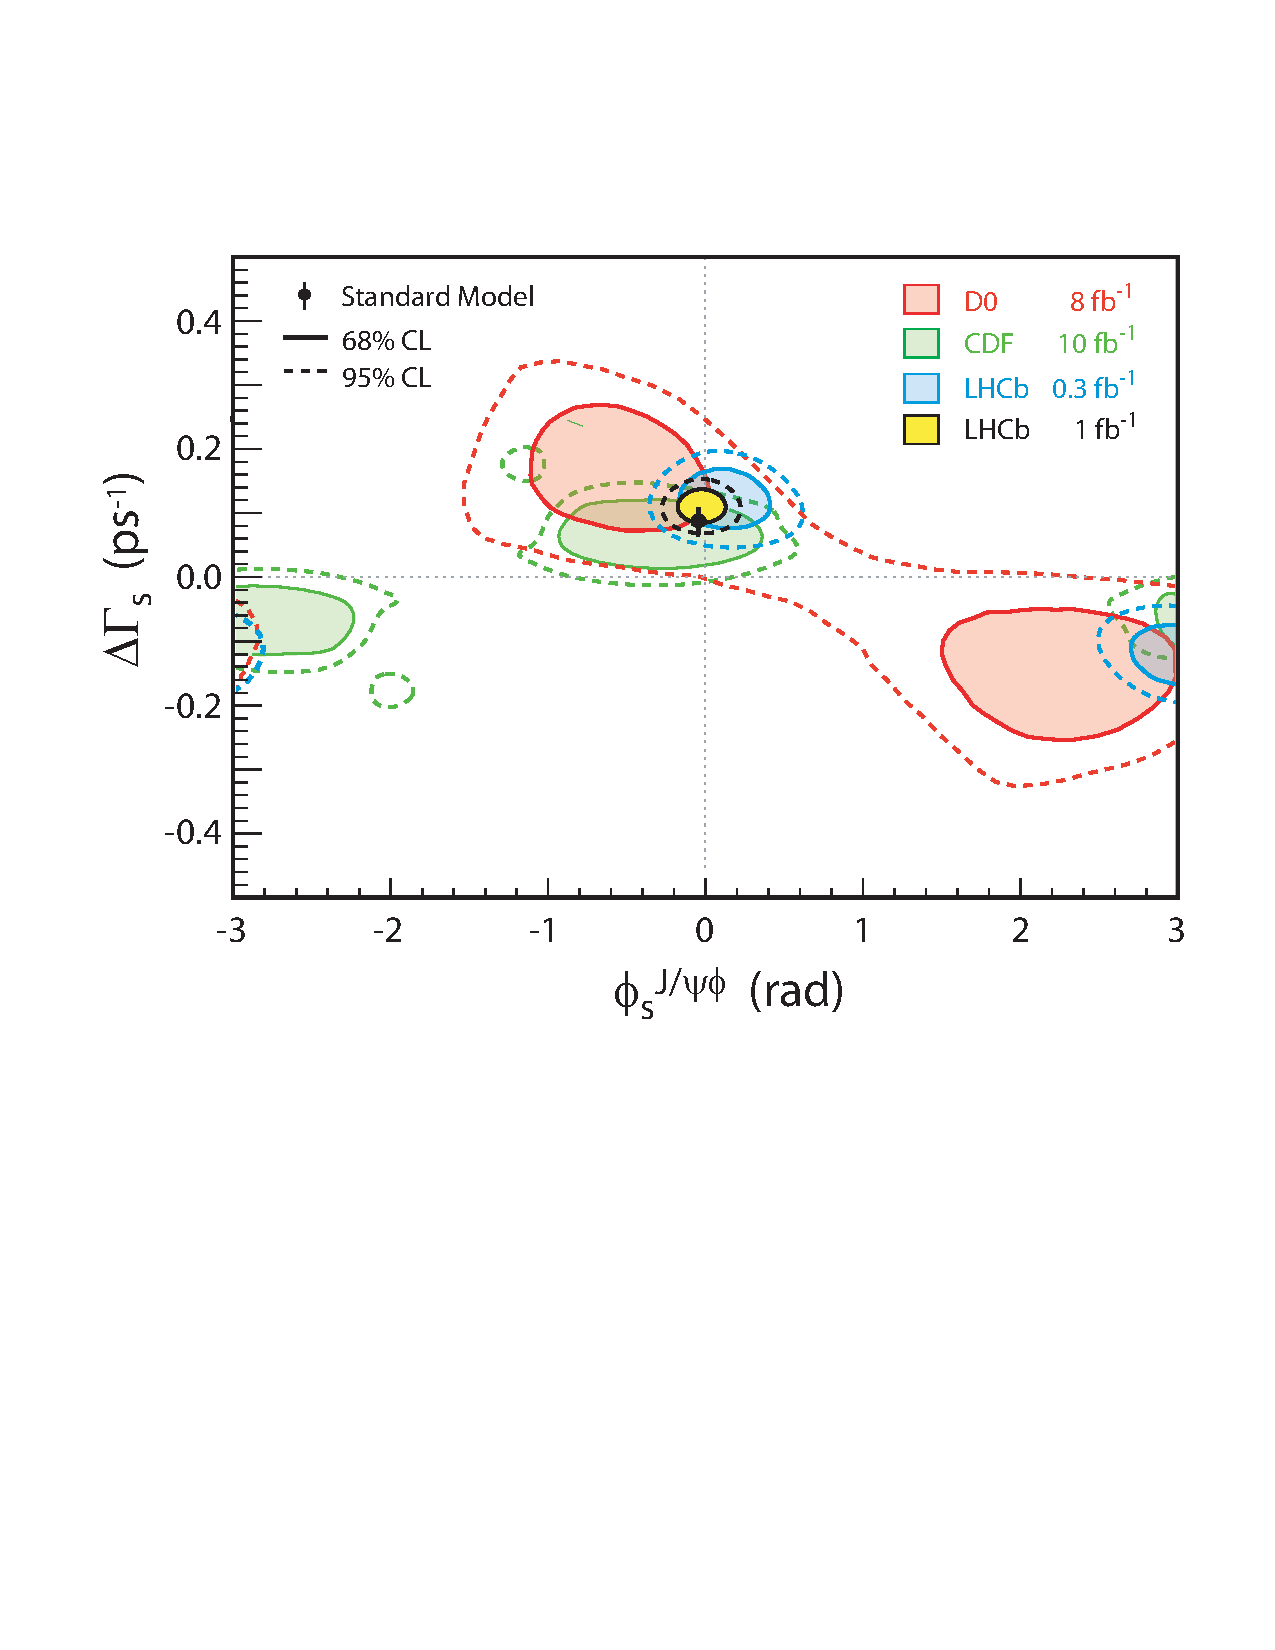
\includegraphics[scale=0.65,bb=50 300 580 700,clip=true]{Roger-plot}
    \vspace*{-1.0cm}
  \end{center}
  \caption{
    \small %captions should be a little bit smaller than main text
    Comparison of our result to those from other experiments.
    Note that the style of this figure differs slightly from that of Figure~\ref{fig:example}}
  \label{fig:roger}
\end{figure}

\clearpage


\newpage
\addcontentsline{toc}{section}{References}
\setboolean{inbibliography}{true}
\bibliographystyle{LHCb}
\bibliography{main,LHCb-PAPER,LHCb-CONF,LHCb-DP,LHCb-TDR}
 

\newpage


\end{document}
